
\documentclass{template/openetcs_report}
% Use the option "nocc" if the document is not licensed under Creative Commons
%\documentclass[nocc]{template/openetcs_article} 
\usepackage{xspace}
\usepackage{graphicx}
\usepackage[draft,nomargin,inline]{fixme}
\usepackage{lscape} 
\usepackage{listings}
\usepackage{placeins}
\usepackage{framed}
\usepackage{booktabs}
\usepackage{amsmath}
\usepackage{amssymb}
\usepackage{stmaryrd}
\usepackage[pdftex]{hyperref}

\numberwithin{figure}{chapter}
\numberwithin{table}{chapter}
\usepackage{float}
\floatstyle{plain}
\newfloat{listing}{thp}{lop1}[chapter]
\floatname{listing}{Listing}

\renewcommand\floatpagefraction{.90}
\renewcommand\topfraction{.90}
\renewcommand\bottomfraction{.90}
\renewcommand\textfraction{.1}
\setlength{\unitlength}{1mm}


%user specified macros


\newcommand{\VV}{Verification \& Validation\xspace}
\newcommand{\vv}{verification \& validation\xspace}

\def\CC{{C\nolinebreak[4]\hspace{-.05em}\raisebox{.4ex}{\tiny\bf ++}}}

\newcommand{\adhesion}{\mbox{\inl{AdhesionFactor}}\xspace}

\newcommand{\bitwalker}{\mbox{\texttt{Bitwalker}}\xspace}

\newcommand{\poke}{\mbox{\texttt{Bitwalker\_Poke}}\xspace}
\newcommand{\peek}{\mbox{\texttt{Bitwalker\_Peek}}\xspace}
\newcommand{\acsl}{\mbox{\textsf{ACSL}}\xspace}
\newcommand{\isoc}{\mbox{\textsf{C}}\xspace}
\newcommand{\framac}{\mbox{\textsf{Frama-C}}\xspace}
\newcommand{\framacwp}{\mbox{\textsf{Frama-C\slash WP}}\xspace}
\newcommand{\why}{\mbox{\textsf{Why}}\xspace}
\newcommand{\wpframac}{\mbox{\textsf{WP}}\xspace}
\newcommand{\altergo}{\mbox{\textsf{Alt-Ergo}}\xspace}
\newcommand{\qed}{\mbox{\textsf{Qed}}\xspace}
\newcommand{\cvc}{\mbox{\textsf{CVC4}}\xspace}
\newcommand{\z}{\mbox{\textsf{Z3}}\xspace}
\newcommand{\coq}{\mbox{\textsf{Coq}}\xspace}
\newcommand{\cealist}{\mbox{\textsf{CEA LIST}}\xspace}
\newcommand{\fokus}{\mbox{\textsf{Fraunhofer FOKUS}}\xspace}

\newcommand{\inl}[1]{\lstinline[style=inline]{#1}}


%Defining C-Code Environment

\usepackage{courier} 
\usepackage{listings}
\usepackage{color} 

% fix bug with listing under texlive-2014
% see https://lists.debian.org/debian-tex-maint/2014/06/msg00209.html

\makeatletter
\renewcommand\lstinline[1][]{%
  \leavevmode\bgroup % \hbox\bgroup --> \bgroup
  \def\lst@boxpos{b}%
  \lsthk@PreSet\lstset{flexiblecolumns,#1}%
  \lsthk@TextStyle
  \ifnum\iffalse{\fi`}=\z@\fi
  \@ifnextchar\bgroup{%
  \ifnum`{=\z@}\fi%
  \afterassignment\lst@InlineG \let\@let@token}{%
  \ifnum`{=\z@}\fi\lstinline@}}
\makeatother


%\definecolor{darkred}		{rgb}{0.60,0.00,0.00}
\definecolor{coACSLBehavior}	{rgb}{0.30,0.00,0.00}
\definecolor{coASCL}		{rgb}{0.00,0.10,0.00}
\definecolor{coASCLKeyword}	{rgb}{0.00,0.10,0.10}
\definecolor{darkgreen}		{rgb}{0.00,0.40,0.00}
%\definecolor{red}		{rgb}{0.98,0.00,0.00}
\definecolor{darkblue}		{rgb}{0.00,0.00,0.60}
%\definecolor{lightblue}		{rgb}{0.60,0.80,1.00}
%\definecolor{lightred}		{rgb}{1.00,0.60,0.60}
\definecolor{coCKeyword}	{rgb}{0.00,0.00,0.60}

\lstdefinestyle{acsl-block}
{	emph=[1]{assert, assumes, assigns, axiom, axiomatic, decreases, ensures,
                 ghost, invariant, lemma, logic, loop, predicate,
		 reads, requires, variant},
	emphstyle=[1]{\bfseries\color{coASCLKeyword}},
	emph=[2]{behavior, behaviors, complete, disjoint, for:},
	emphstyle=[2]{\bfseries\color{coACSLBehavior}},
	emph=[3]{typedef, int, char, integer, real, bool, size_type, value_type, uint8_t,  uint64_t},
	emphstyle=[3]{\bfseries\color{coCKeyword}},
	escapeinside={//`}{`//},
	morecomment=*[l][\color{coASCL}]{//@},
	morecomment=*[s][\color{coASCL}]{/*@}{*/},
	moredelim=*[is][\bfseries]{|*}{*|},
	%emphstyle=[3]{\ttfamily}
	}

\lstdefinestyle{func-decl}
{	emph=[1]{assert, assumes, assigns, axiom, axiomatic, decreases, ensures,
                 ghost, invariant, lemma, logic, loop, predicate,
		 reads, requires, variant},
	emphstyle=[1]{\bfseries\color{coASCLKeyword}},
	emph=[2]{behavior, behaviors, complete, disjoint, for:},
	emphstyle=[2]{\bfseries\color{coACSLBehavior}},
	emph=[3]{integer, real, size_type, value_type},
	emphstyle=[3]{\bfseries\color{coCKeyword}},
	escapeinside={//`}{`//},
	morecomment=*[l][\color{coASCL}]{//@},
	morecomment=*[s][\color{coASCL}]{/*@}{*/},
	moredelim=*[is][\bfseries]{|*}{*|},
    frame=none,
    numbers=none
	%emphstyle=[3]{\ttfamily}
	}

\lstdefinestyle{acsl-inline}
{	emph=[1]{assert,assigns, assumes, axiom, axiomatic, decreases, ensures, ghost, invariant, lemma, logic, loop,
             predicate, reads, requires, return, variant },
	emphstyle=[1]{\bfseries\color{coASCLKeyword}},
	emph=[2]{behavior, behaviors, complete, disjoint, for:},
	emphstyle=[2]{\bfseries\color{coACSLBehavior}},
	emph=[3]{typedef, int, char, integer, real, bool, size_type, value_type, uint8_t,  uint64_t},
	emphstyle=[3]{\bfseries\color{coCKeyword}},
	morecomment=*[l][\color{coASCL}]{//@},
	morecomment=*[s][\color{coASCL}]{/*@}{*/},
	moredelim=*[is][\bfseries]{|*}{*|}
}

\lstdefinestyle{inline}
{      % basicstyle = \ttfamily\small\color{coASCL},
	keywordstyle = \ttfamily\normal\color{coASCL},
	stringstyle=\color{coASCL},
	style=acsl-inline,
	breaklines= false
}

\lstset{%
  language=C++,
  defaultdialect=ansi,
  basicstyle=\footnotesize\ttfamily,
  commentstyle=\small\color{darkgreen},
  keywordstyle=\small\bfseries\color{darkblue},
  stringstyle=\small\color{darkgreen},
  tabsize = 2,
  showspaces=false,
  showtabs=false,
  columns=fixed,  
  frame=none,  
  breaklines=true,
  showstringspaces=false,
  xleftmargin=0.2cm,
  %rangeprefix=//label, % to specify a certain range from a file
  %rangesuffix=;, % to be shown
  %includerangemarker=false,
	numbers=none
}


\graphicspath{{./template/}{.}{./images/}}
\begin{document}
\frontmatter
\project{openETCS}

%Please do not change anything above this line
%============================
% The document metadata is defined below

%assign a report number here
\reportnum{OETCS/WP4/D4.3.2}

%define your workpackage here
\wp{Work Package 4: ``Validation \& Verification Strategy''}

%set a title here
\title{Final Report on Validation and Verification Report of Implementation/Code}

%set a subtitle here
%\subtitle{Description of Work}

%set the date of the report here
\date{March 2015}

%define a list of authors and their affiliation here

\creatorname{Jens Gerlach}
\creatoraffil{Fraunhofer FOKUS}

\techassessorname{Virgile Prevosto}
\techassessoraffil{CEA LIST}

\qualityassessorname{Abdelnasir Mohamed}
\qualityassessoraffil{AEbt}

\approvalname{Klaus-R\"udiger Hase}
\approvalaffil{DB Netz}

\author{Jens Gerlach}
\affiliation{Fraunhofer FOKUS\\
  Kaiserin-Augusta-Allee 31 \\
  10589 Berlin, Germany\\
  jens.gerlach@fokus.fraunhofer.de \\
  www.fokus.fraunhofer.de}

\author{Izaskun de la Torre}
\affiliation{Software Quality Systems S.A.}

% define the coverart
\coverart[width=350pt]{openETCS_EUPL}

%define the type of report
\reporttype{Intermediate report}


\begin{abstract}
  This work package will comprise the activities concerned with
  verification and validation within openETCS. This includes \vv of
  development artifacts, that is, showing that models and code
  produced correctly express or implement what they are supposed
  to. And also, methods and tools to perform such tasks will be
  evaluated with the goal of assembling a suitable method and tool
  chain to support a full development.
\end{abstract}

%=============================
%Do not change the next three lines
\maketitle
\tableofcontents
\listoffiguresandtables
\clearpage
\listof{listing}{List of code examples}
\listoffixmes
\cleardoublepage
%=============================

% The actual document starts below this line
%=============================

\mainmatter
%Start here

\section{Introduction}\label{sec:intro}
% ==========================================================================

\subsection{A Test Model for the ETCS Ceiling Speed Monitor}
In 2011 the {\it model-based testing benchmarks website} www.mbt-benchmarks.org has been 
created with the objective to publish test models that may serve as challenges or benchmarks 
for validating testing theories   and for comparing the capabilities of model-based testing (MBT) tools~\cite{pel2011a}.
In this technical report a novel contribution to this website is presented, a SysML model
of the Ceiling Speed Monitor (CSM) which is part of the European Vital Computer (EVC), the onboard controller of trains conforming to the European Train Control System (ETCS) standard~\cite{ETCS}. In    Section~\ref{sec:ceil} the functional objectives for the CSM are described, and in Section~\ref{sec:modeldesc} the detailed model description is provided. 

The static and behavioural semantics of SysML models have been defined in~\cite{SysML12,uml_2_4} in a semi-formal way, leaving certain ``semantic variation points'' open, so that they can be adjusted according to project-specific requirements. For automated model-based testing, however, a strictly formal semantics is required, so that concrete test data can be calculated from the model's transition relation using constraint solving techniques~\cite{peleska2013ictss}. 
We therefore describe in Section~\ref{sec:transrel} how a formal behavioural semantics is derived for the CSM model and present the associated transition relation in propositional form.

We use state transition systems (STS) for encoding the operational semantics of concrete
modelling formalisms like SysML. STS are widely known from the field of model checking~\cite{clarke_em-etal:1999a}, because their extension into Kripke Structures allows for effective data abstraction techniques. The latter are also applied for equivalence class testing. 
Since state transition systems are a means for semantic representation, testing theories elaborated for STS are applicable for all concrete formalisms whose behavioural semantics can be expressed by STS. In~\cite{d341} it is shown how the semantics of general SysML models and models of a process algebra are encoded as STS. In this technical report we illustrate  how this is achieved for the concrete case of the CSM SysML model.

% ==========================================================================
\subsection{Equivalence Class Partition Testing for the CSM}

The CSM represents a specific test-related challenge: its behaviour depends on actual and allowed speed, and these have conceptually real-valued data domains, so that -- even when   discretising
the input space -- it would be infeasible to exercise all possible combinations of 
inputs on the system under test (SUT). Therefore equivalence class partition (ECP)
 testing strategies have 
to be applied for testing the CSM. While these strategies are well-adopted  in a heuristic manner
in today's industrial test campaigns, practical application of equivalence class testing still lacks 
formal justification of the equivalence classes selected and the sequences of class representatives 
selected as test cases: standard text books used in industry, for example~\cite{spillner2006}, 
only explain the generation of input equivalence class tests for   systems, where the 
SUT reaction to an input class representative is independent on the internal state. Moreover, the systematic calculation of classes from models, as well as their formal justification with respect to
test strength and coverage achieved, is not yet part of today's best practices in industry. 

In contrast to this, formal approaches to equivalence class testing have been studied in the formal methods communities; references to these results  are given in Section~\ref{sec:related}.
In the second main part of this report (Section~\ref{sec:iecpstart}) we therefore describe a recent formal technique for equivalence class testing and its application to testing the CSM. The theoretical 
foundations of this strategy have been published by two of the authors in~\cite{peleska2013ictss}. 
This technical report illustrates its practical application and presents first evaluation details using a 
prototype implementation in an existing MBT tool; the ECP tests are  compared to test results obtained when applying other MBT coverage strategies, such as transition cover or MC/DC coverage (Section~\ref{sec:conventionaltests}). 


% ==========================================================================
\subsection{Fault Models and Completeness Results}


Our ECP strategy
introduces test suites depending on {\it fault models}. This well adopted notion has first been 
introduced in the field of finite state machine (FSM) testing~\cite{petrenko1996}, but is also applicable
to other formal modelling techniques. A fault model consists of a reference model, a conformance relation and a fault domain. The latter is a collection of models whose behaviour may or may not be
consistent to the reference model in the sense of the conformance relation. The test suites generated 
by the ECP strategy described here are {\it complete} with respect to the given fault model: each
system of the fault domain which conforms to the reference model will pass all the generated tests
(this means that the test suite is {\it sound}), and each system in the fault domain that violates the
conformity to the reference model will fail at least  once when tested according to the test suite (the test suite is {\it exhaustive}). 




%%% @todo open proof strategy of the openETCS project




\cleardoublepage

\chapter{An introduction to formal verification with \framacwp}
\label{sec:frama-c}

Frama-C is a platform dedicated to source-code analysis of C software.
It has a plug-in architecture and can thus be easily extended to 
different kinds of analyses.
The WP plugin of Frama-C allows one to formally verify that a piece of
C code satisfies its specification.
This implies, of course, that the user provides a \emph{formal specification}
of what the implementation is supposed to do.
Frama-C comes with its own specification language ACSL which stands for
\emph{ANSI\slash ISO C Specification Language}.
In order to help potential users to master ACSL we discuss in this chapter 
a very simple C function \inl{abs_int} that implements the computation of
the absolute value for objects of type~\inl{int}.

\begin{itemize}
\item
In Section~\ref{sec:first-steps} we will present a straightforward
specification of \inl{abs_int}.
We discuss the reasons why \framacwp is not able to verify that our
implementation satisfies this specification in Section~\ref{sec:framac-failure}.

\item 
In Section~\ref{sec:contract-sharpening} we provide a more precise
specification that can be verified by \framacwp.
In Section~\ref{sec:separating-spec-impl} we explain
how \framac supports---by allowing the separation of the specification from the 
implementation---good software engineering practices.

\item
Sections~\ref{sec:modular-verification} and~\ref{sec:side-effects}
discuss, respectively,
how \framacwp supports \emph{modular verification} and the
formal treatment of \emph{side effects}.
\end{itemize}

\clearpage

\section{First steps}
\label{sec:first-steps}

We will consider the function that computes the absolute value $|x|$
of an integer $x$.
In order to avoid name clashes with the function \inl{abs} in C standard library
we use the name \inl{abs_int}.

The mathematical definition of absolute value is very simple
\begin{align}
\label{eq:abs}
   |x| &= \left\{
            \begin{array}{rl}
               x  & \text{if $x \geq 0$} \\
               -x & \text{if $x < 0$}
            \end{array}
          \right.
\end{align}

A straightforward implementation of \inl{abs_int} is shown in Listing~\ref{lst:abs}.

\begin{listing}[hbt]
\begin{minipage}{\textwidth}
\lstinputlisting[style=acsl-block ]{./Abs/abs.c}
\end{minipage}
\caption{\label{lst:abs} An implementation of the absolute value function}
\end{listing}

In order to demonstrate that this implementation is correct we have to provide
a formal specification.
Listing~\ref{lst:abs1} shows our first attempt for an ACSL specification of \inl{abs_int} that
is based on the mathematical definition of the function $x \mapsto |x|$ in Equation~\ref{eq:abs}.

\begin{listing}[hbt]
\begin{minipage}{\textwidth}
\lstinputlisting[style=acsl-block ]{./Abs/abs1.c}
\end{minipage}
\caption{\label{lst:abs1} A first attempt to formally specify \inl{abs_int}}
\end{listing}

\FloatBarrier

The first thing to note is that ACSL specifications---or \emph{contracts}---are placed in special C comments
(they start with \inl{/*@}).
Thus, they do not interfere with the executable code.
The \inl{ensures} clause in the specification expresses \emph{postconditions},
that is, properties that should be guaranteed \emph{after} the execution
of \inl{abs_int}.
The ACSL reserved word \inl{\\result} is used to refer to the return value of a C function.
Note that we use the usual C operators \inl{==} and \inl{<=} to express equalities and inequalities
in the specification.
There is also an additional operator \inl{==>} which expresses logical implication.

\section{Why can \framacwp not verify such a simple function?}
\label{sec:framac-failure}

Although the specification and implementation in Listing~\ref{lst:abs1} look perfectly right, 
\framacwp cannot verify that the implementation actually satisfies its specification.


The reason becomes clear if we look at some actual return values of \inl{abs_int}.
Listing~\ref{lst:test_abs} shows our test code whose output is
listed in Table~\ref{tbl:test_abs_output}.

\begin{listing}[hbt]
\begin{minipage}{\textwidth}
\lstinputlisting[style=acsl-block ]{./Abs/test_abs.c}
\end{minipage}
\caption{\label{lst:test_abs} Some simple test cases for \inl{abs_int}}
\end{listing}

%\clearpage

\begin{table}[hbt]
\begin{center}
\begin{tabular}{|r|r|c|}
\hline
\inl{x} &  \inl{abs_int(x)} & Remark \\ \hline\hline
0	&	0 & \checkmark \\ \hline
1	&	1 & \checkmark \\ \hline
10	&	10 & \checkmark \\ \hline
2147483647	&	2147483647 & \checkmark \\ \hline
-1	&	1 & \checkmark \\ \hline
-10	&	10 & \checkmark \\ \hline
-2147483648	&	-2147483648 & $\lightning$ \\ \hline
\end{tabular}
\end{center}
\caption{\label{tbl:test_abs_output} Test results for \inl{abs_int}}
\end{table}

\FloatBarrier

The offending value is in the last line of Table~\ref{tbl:test_abs_output}
which basically states that \inl{abs_int(INT_MIN)} equals \inl{INT_MIN}
whereas it should equal \inl{-INT_MIN}.
The problem is that the type \inl{int} only present a 
finite subset of the (mathematical) integers.
Many computers use a two's-complement representation of integers
which covers the range $[-2^{31}\ldots 2^{31}-1]$ on a 32-bit machine.
On such a machine \inl{-INT_MIN} cannot be  represented by a value
of the type~\inl{int}.

In a specification, \framacwp interprets integers as mathematical entities.
Consequently, there is no such thing as an \emph{arithmetic overflow} when
adding or multiplying them.
In other words,
\framacwp is perfectly right not being able to verify that \inl{abs_int}
satisfies the contract in Listing~\ref{lst:abs1}. Indeed, the 
implementation does not respect the given specification.


\section{Sharpening the contract of \inl{abs_int}}
\label{sec:contract-sharpening}

It is of course well known that the operation \inl{-x} can overflow
and it is the fact that \framacwp can detect such overflows that 
helps to prevent incorrect verification results.

The GNU Standard C Library clearly states that the absolute value of
\inl{INT_MIN} is undefined.\footnote{%
  See \url{http://www.gnu.org/software/libc/manual/html_node/Absolute-Value.html}
}
Under \textsf{OSX}, the manual page of \inl{abs} mentions under the field of ``Bugs'':
%
\begin{small}
\begin{verbatim}
    The absolute value of the most negative integer remains negative.
\end{verbatim}
\end{small}

Thus, our formal specification should exclude the value \inl{INT_MIN}
from the set of admissible value to which \inl{abs_int} can be applied.
In ACSL, we can use the \inl{requires} clause to express \emph{preconditions}
of a function.
Listing~\ref{lst:abs1a} shows an extended contract of \inl{abs_int}
that takes the limitations of the type \inl{int} into account.

\begin{listing}[hbt]
\begin{minipage}{\textwidth}
\lstinputlisting[style=acsl-block ]{./Abs/abs1a.c}
\end{minipage}
\caption{\label{lst:abs1a} Taking integer overflows into account}
\end{listing}

\FloatBarrier

\framacwp is now capable to verify that the implementation of
\inl{abs_int} satisfies the specification of Listing~\ref{lst:abs1a}.

There is an important lesson that can be learned here:
\begin{framed}
\label{lesson}
Sometimes developers provide source code and imagine that a tool
like \framacwp can verify the correctness of their implementation.
In order to fulfill its task, however, \framacwp needs an ACSL specification. 
Such a specification---which must be based on a reasonably precise description of the
admissible inputs and expected behavior---has to come from the \emph{requirements}
of the software and is not magically discovered from the source code by \framacwp.
The code does what it does. 
In order to verify that the code does what someone expects, these expectations
must be clearly expressed, that is, they must be formally specified.
\end{framed}

%\clearpage 

Of course, it might not always be the goal to verify the complete functionality of a
piece of software.
Sometimes, it is enough to ensure that individual software components
cause no runtime errors, that is, arithmetic overflows or invalid pointer accesses.
\framacwp can also be used in this situation.
Under the terms of the following minimal specification in 
Listing~\ref{lst:abs1b}, \framacwp can verify that no runtime error will occur.

\begin{listing}[hbt]
\begin{minipage}{\textwidth}
\lstinputlisting[style=acsl-block ]{./Abs/abs1b.c}
\end{minipage}
\caption{\label{lst:abs1b} Minimal contract to ensure the absence of runtime errors in \inl{abs_int}}
\end{listing}

%\clearpage

\section{Separating specification and implementation}
\label{sec:separating-spec-impl}

Before we continue exploring more advanced specification and verification
capabilities of \framacwp we turn to a simple software engineering question.

It is common practice to put function prototypes into ``\inl{.h}'' files and
keep the implementation in files ending in~``\inl{.c}''.
\framacwp supports this separation of specification and implementation.
Listing~\ref{lst:abs2-h} shows the file \inl{abs2.h} which contains
a declaration of \inl{abs_int} together with an attached ACSL specification.

\begin{listing}[hbt]
\begin{minipage}{\textwidth}
\lstinputlisting[style=acsl-block ]{./Abs/abs2.h}
\end{minipage}
\caption{\label{lst:abs2-h} Specifying a function prototype in a header file}
\end{listing}

Listing~\ref{lst:abs2-c} shows the specification of \inl{abs_int} in a~\inl{.c} file.
Note that the file \inl{abs2.h} with the specification is included by this file.
\framacwp can verify that this implementation satisfies the contract in
Listing~\ref{lst:abs2-h}.



\begin{listing}[hbt]
\begin{minipage}{\textwidth}
\lstinputlisting[style=acsl-block ]{./Abs/abs2.c}
\end{minipage}
\caption{\label{lst:abs2-c} Implementation at a different location than the specification}
\end{listing}

We remark, that the definition of a very small function like \inl{abs_int} would normally
be placed in a header file so that a compiler can inline the function definition
at the call site.

%\clearpage

\section{Modular verification}
\label{sec:modular-verification}

We now look at a simple example in which our function \inl{abs_int} is used.
More precisely, we include in Listing~\ref{lst:use_abs2-1} the
header file from Listing~\ref{lst:abs2-h} which contains an ACSL specification of \inl{abs_int}.

\begin{listing}[hbt]
\begin{minipage}{\textwidth}
\lstinputlisting[style=acsl-block ]{./Abs/use_abs2_1.c}
\end{minipage}
\caption{\label{lst:use_abs2-1} A simple example of modular verification}
\end{listing}

\FloatBarrier

When \framacwp tries to verify the code in Listing~\ref{lst:use_abs2-1},
then it actually tries to establish whether at each program location where
it is called the \emph{preconditions} of \inl{abs_int} are satisfied.
Based on the specification of \inl{abs_int},
\framacwp can indeed verify that for the first three calls the preconditions are fulfilled.
For the last call this verification fails because the value \inl{INT_MIN}
is explicitly excluded by the specification in Listing~\ref{lst:abs2-h}.

Note that the \emph{implementation} of \inl{abs_int}
does not play any role in determining whether it is safe to
call the function in a particular context.
This is what we call \emph{modular verification}: a function can be verified in
isolation whereas code that calls the function only uses the function contract.

This also means that in a situation as in Listing~\ref{lst:use_abs2-2},
where nothing is known about the argument of \inl{abs_int}, 
\framacwp cannot establish that the precondition of \inl{abs_int} is satisfied
or, in other words, that \inl{x > INT_MIN} holds.

\begin{listing}[hbt]
\begin{minipage}{\textwidth}
\lstinputlisting[style=acsl-block ]{./Abs/use_abs2_2.c}
\end{minipage}
\caption{\label{lst:use_abs2-2} Another example of modular verification}
\end{listing}

\FloatBarrier

If, on the other hand, we have precise information on the arguments at call site, then \framacwp can exploit the specification of 
\inl{abs_int} in order derive some interesting properties.
As an example, we consider the code fragment in Listing~\ref{lst:use_abs2-3}.
Here, \framacwp can verify that the assertion after 
the call of \inl{abs_int} is correct.


\begin{listing}[hbt]
\begin{minipage}{\textwidth}
\lstinputlisting[style=acsl-block ]{./Abs/use_abs2_3.c}
\end{minipage}
\caption{\label{lst:use_abs2-3} A more complex example of modular verification}
\end{listing}

Note that this assertion is a \emph{static} one, that is, it is
an ACSL annotation that resides inside a comment and does not affect
the execution of the code in Listing~\ref{lst:use_abs2-3}.
Also note that unlike to C~code, \emph{relation chains} can be used both in function
contracts and assertions.

%\clearpage

\section{Dealing with side effects}
\label{sec:side-effects}

Listing~\ref{lst:abs3a1} shows an implementation of \inl{abs_int}
that writes as a side effect the argument~\inl{x} to a global variable~\inl{a}.
A natural question is to ask whether this implementation with a side effect
also satisfies the specification.

\begin{listing}[hbt]
\begin{minipage}{\textwidth}
\lstinputlisting[style=acsl-block ]{./Abs/abs3a1.c}
\end{minipage}
\caption{\label{lst:abs3a1} An implementation with side effects}
\end{listing}

\FloatBarrier

Before we answer this question we consider various uses for side effects.
There are of course legitimate uses for side effects.
The assignment to a memory location outside the scope of the function
might be meaningful because an error condition is reported or because
some data are logged as in Listing~\ref{lst:abs3logging1}.

\begin{listing}[hbt]
\begin{minipage}{\textwidth}
\lstinputlisting[style=acsl-block ]{./Abs/abs3logging1.c}
\end{minipage}
\caption{\label{lst:abs3logging1} Calling a logging function from \inl{abs_int}}
\end{listing}

If \framacwp attempts to verify the code in Listing~\ref{lst:abs3logging1},
then it issues the following warning:
%
\begin{small}
\begin{verbatim}
    Neither code nor specification for function logging,
    generating default assigns from the prototype
\end{verbatim}
\end{small}
%
Thus, it points out that the called function \inl{logging} should have a proper
specification that clearly indicates its side effects.

There are, on the other hand, also good reasons to minimize or even forbid side 
effects:

\begin{itemize}
\item
Imagine a malicious password checking function that writes the password to
a global variable.

\item
Another reason is that side effects can make it harder to understand what 
the real consequences of a function call are.
In particular, one must be concerned about unintended consequences that
are caused by side effects
The norm IEC 61508 therefore requests in the context of software module testing
and integration testing:

\begin{quote}
To show that all software modules,
elements and subsystems interact correctly
to perform their intended function and do not perform unintended functions
(see also.~\cite[\S 7.4.7.2,\S 7.7.2.9]{IEC-61508-3})
\end{quote}

Of course, it is quite difficult to ensure by testing alone that something does \emph{not} happen.
\end{itemize}

To come back to our question about Listing~\ref{lst:abs3a1} it is important
to understand that \framacwp verifies that the implementation shown there
satisfies the specification.

If one wishes to forbid that a function changes global variables
one can use an \inl{assigns \\nothing} clause as shown in Listing~\ref{lst:abs3a2}.
\framacwp will then point out that this implementation prevents
the verification of the assigns clause.

\begin{listing}[hbt]
\begin{minipage}{\textwidth}
\lstinputlisting[style=acsl-block ]{./Abs/abs3a2.c}
\end{minipage}
\caption{\label{lst:abs3a2} Specifying the absence of side effects}
\end{listing}


\FloatBarrier

Of course, an all-or-nothing-approach to side effects is not very helpful
for the verification of real-life software.
Listing~\ref{lst:abs3a3} shows how the \inl{assigns} clause of a
specification can name the exact memory location that the
function is allowed to modify.

\begin{listing}[hbt]
\begin{minipage}{\textwidth}
\lstinputlisting[style=acsl-block ]{./Abs/abs3a3.c}
\end{minipage}
\caption{\label{lst:abs3a3} Finer control of side effects}
\end{listing}

Note however that \inl{assigns a} does not imply that a write to \inl{a}
necessarily occurs during the execution of \inl{abs}. On the other hand, any
other memory location must stay unchanged between the initial state
and the final state of \inl{abs}.

\cleardoublepage


\chapter{ETCS data packets}
\label{sec:packets}

In the following, we give a top-down presentation of the OpenETCS
Decoder software.
We discuss the highest, i.e.\ the data packet level, in this chapter;
Chapter~\ref{cha:bitstream} elaborates on some intermediate, and
Appendix~\ref{cha:low-level bitstream} on the lowest level.

On the data packet level, a total of \fxfatal{ANZAHL} different packets
are defined, each by a \lstinline{struct} declaration in \lstinline{C}.
We exemplify our discussion on the alphabetically first packet,
\inl{AdhesionFactor} (Section~\ref{sec:adhesionfactor}), and give some
comments on considerations with respect to other packets
(Section~\ref{sec:other packets}).

In order to cope with the similarity of specification, implementation,
and verification tasks for all packets, we have chosen to automatically 
generate \fxfatal{Was genau? struct declaration, contract, ...} from the
ETCS Subset 026 requirements description.\fxfatal{Name improvisiert}

\section{Formal specification of \inl{AdhesionFactor}}
\label{sec:adhesionfactor}

\subsection{\inl{AdhesionFactor} in ETCS}
\label{sec:adhesionfactor-etcs}

Subset~026 defines package \emph{adhesion factor} (packet 71) as shown in 
Table~\ref{tbl:adhesion-factor}.

\begin{table}[hbt]
\begin{center}
\begin{tabular}{|l|r|}
\hline
\textbf{variable name} & \textbf{number of bits}\\
\hline
\inl{NID_PACKET} & 8 \\
\hline
\inl{Q_DIR} & 2 \\
\hline
\inl{L_PACKET} & 13 \\
\hline
\inl{Q_SCALE} & 2 \\
\hline
\inl{D_ADHESION} & 15 \\
\hline
\inl{L_ADHESION} & 15 \\
\hline
\inl{M_ADHESION} & 1 \\
\hline
\end{tabular}
\end{center}
\caption{\label{tbl:adhesion-factor} Packet \adhesion as defined by ETCS}
\end{table}


\subsection{The type \inl{AdhesionFactor}}
\label{sec:adhesionfactor-type}

Listing~\ref{lst:adhesionfactor-type} shows the definition of type
\inl{AdhesionFactor} as it is generated from the ETCS specification shown in Section~\ref{sec:adhesionfactor-etcs}.

\begin{listing}[hbt]
\begin{minipage}{0.99\textwidth}
\begin{lstlisting}[style=acsl-block]
struct AdhesionFactor
{
    PacketHeader header;

    // TransmissionMedia=Any
    // This packet is used when the trackside requests a change of
    // the adhesion factor to be used in the brake model.
    // Packet Number = 71

    uint64_t  Q_DIR;            // # 2
    uint64_t  L_PACKET;         // # 13
    uint64_t  Q_SCALE;          // # 2
    uint64_t  D_ADHESION;       // # 15
    uint64_t  L_ADHESION;       // # 15
    uint64_t  M_ADHESION;       // # 1
};

typedef struct AdhesionFactor AdhesionFactor;
\end{lstlisting}
\end{minipage}
\caption{\label{lst:adhesionfactor-type}Definition of the type \inl{AdhesionFactor}}
\end{listing}

\FloatBarrier  % forces the output of listings/tables

\subsection{\acsl predicates \inl{AdhesionFactor}}
\label{sec:adhesionfactor-predicates-bitsize}

Listing~\ref{lst:adhesionfactor-predicates-bitsize} shows the definition of
the logic functions \inl{BitSize} and \inl{MaxBitSize} for \inl{AdhesionFactor}.
The former function uses a macro that contains the size of \inl{AdhesionFactor} in bits.
The functions are used in Listing~\ref{lst:adhesionfactor-decodebit} and
Listing~\ref{lst:adhesionfactor-encodebit} where the overloading of the
logic predicates allows for a more generic \acsl contract for the \inl{EncodeBit} and
\inl{DecodeBit} functions.

\begin{listing}[hbt]
\begin{minipage}{0.99\textwidth}
\begin{lstlisting}[style=acsl-block]
/*@
    logic integer BitSize{L}(AdhesionFactor* p) = ADHESIONFACTOR_BITSIZE;

    logic integer MaxBitSize{L}(AdhesionFactor* p) = BitSize(p);
*/
\end{lstlisting}
\end{minipage}
\caption{\label{lst:adhesionfactor-predicates-bitsize}Definition of the \inl{BitSize} predicates for \inl{AdhesionFactor}}
\end{listing}

\FloatBarrier

\label{sec:adhesionfactor-predicates-invariant}

Listing~\ref{lst:adhesionfactor-predicates-invariant} shows the definition of the
\inl{Invariant} predicate for \inl{AdhesionFactor}.
The predicate is the conjunction of the (trivial) \inl{Invariant(uint64_t)} predicates
of all members of on object of type \inl{AdhesionFactor}.

\begin{listing}[hbt]
\begin{minipage}{0.99\textwidth}
\begin{lstlisting}[style=acsl-block]
/*@
    predicate Invariant(AdhesionFactor* p) =
      Invariant(p->Q_DIR)             &&
      Invariant(p->L_PACKET)          &&
      Invariant(p->Q_SCALE)           &&
      Invariant(p->D_ADHESION)        &&
      Invariant(p->L_ADHESION)        &&
      Invariant(p->M_ADHESION);
*/
\end{lstlisting}
\end{minipage}
\caption{\label{lst:adhesionfactor-predicates-invariant}Definition of the \inl{Invariant} predicate for \inl{AdhesionFactor}}
\end{listing}

\FloatBarrier

\label{sec:adhesionfactor-predicates-upperbitsnotset}

%\fxfatal{Make sure that there is an explanation of UpperBitsNotSet in Chapter~\ref{cha:bitstream}}

Listing~\ref{lst:adhesionfactor-predicates-upperbitsnotset} shows the definition
of the \inl{UpperBitsNotSet} predicate for \inl{AdhesionFactor}.
The predicate \inl{UpperBitsNotSet(AdhesionFactor*)} evaluates to true
if and only if the values of all members of \inl{AdhesionFactor}
fit into their assigned numbers of bits.
This functionality is ensured by the conjunction of the \inl{UpperBitsNotSet(uint64_t, uint32_t)} predicate,
which is explained in Appendix~\ref{sec:bit operations in framac}, for all members of \inl{AdhesionFactor}.

\begin{listing}[hbt]
\begin{minipage}{0.99\textwidth}
\begin{lstlisting}[style=acsl-block]
/*@
    predicate UpperBitsNotSet(AdhesionFactor* p) =
      UpperBitsNotSet(p->Q_DIR,            2)   &&
      UpperBitsNotSet(p->L_PACKET,         13)  &&
      UpperBitsNotSet(p->Q_SCALE,          2)   &&
      UpperBitsNotSet(p->D_ADHESION,       15)  &&
      UpperBitsNotSet(p->L_ADHESION,       15)  &&
      UpperBitsNotSet(p->M_ADHESION,       1);
*/
\end{lstlisting}
\end{minipage}
\caption{\label{lst:adhesionfactor-predicates-upperbitsnotset}Definition of the \inl{UpperBitsNotSet} predicate for \inl{AdhesionFactor}}
\end{listing}

\FloatBarrier

\label{sec:adhesionfactor-predicates-separated}

Listing~\ref{lst:adhesionfactor-predicates-separated} shows the definition of 
predicate  \inl{Separated} for \inl{AdhesionFactor}.
The predicate \inl{Separated(stream, p)} is true if and only if 
the two objects \inl{*stream} and \inl{*p} do not overlap in memory.
Thus, writing into the stream will not change \inl{*p} and vice versa.

\begin{listing}[hbt]
\begin{minipage}{0.99\textwidth}
\begin{lstlisting}[style=acsl-block]
/*@
    predicate Separated(Bitstream* stream, AdhesionFactor* p) =
      \separated(stream, p) &&
      \separated(stream->addr + (0..stream->size-1), p);
*/
\end{lstlisting}
\end{minipage}
\caption{\label{lst:adhesionfactor-predicates-separated}Definition of the \inl{Separated} predicate for \inl{AdhesionFactor}}
\end{listing}

\FloatBarrier

\label{sec:adhesionfactor-predicates-equalbits}

%\fxfatal{Make sure that there is an explanation of EqualBits in Chapter~\ref{cha:bitstream}}

Listing~\ref{lst:adhesionfactor-predicates-equalbits} shows the definition of the
\inl{EqualBits} predicate for \inl{AdhesionFactor}.
Based on the ETCS specification, this predicate describes a
relationship between the bits of the individual members
of an object of type \inl{AdhesionFactor} and those of a bit stream.
This predicate will be used to formally describe the transfer of bits
from a bit stream to an object of type \inl{AdhesionFactor} and vice versa.
The definition of the predicate \inl{EqualBits(AdhesionFactor*)} uses
the predicate \inl{EqualBits(uint64_t)}, which is explained
in Section~\ref{sec:bitstream}.

\begin{listing}[hbt]
\begin{minipage}{0.99\textwidth}
\begin{lstlisting}[style=acsl-block]
/*@
    predicate EqualBits(Bitstream* stream, integer pos, AdhesionFactor* p) =
      EqualBits(stream, pos,       pos + 2,   p->Q_DIR)             &&
      EqualBits(stream, pos + 2,   pos + 15,  p->L_PACKET)          &&
      EqualBits(stream, pos + 15,  pos + 17,  p->Q_SCALE)           &&
      EqualBits(stream, pos + 17,  pos + 32,  p->D_ADHESION)        &&
      EqualBits(stream, pos + 32,  pos + 47,  p->L_ADHESION)        &&
      EqualBits(stream, pos + 47,  pos + 48,  p->M_ADHESION);
*/
\end{lstlisting}
\end{minipage}
\caption{\label{lst:adhesionfactor-predicates-equalbits}Definition of the \inl{EqualBits} predicate for \inl{AdhesionFactor}}
\end{listing}

\FloatBarrier

\subsection{Formal specification of \inl{AdhesionFactor_UpperBitsNotSet}}
\label{sec:adhesionfactor-upperbitsnotset}

Listing~\ref{lst:adhesionfactor-upperbitsnotset} shows the contract of the \inl{UpperBitsNotSet}
function for \inl{AdhesionFactor}.
The function contract includes the \inl{requires} clauses, labeled \inl{valid} and \inl{invariant}.
These limit the significance of the \inl{ensures} and \inl{assigns} clauses to
the \inl{AdhesionFactor} objects that also satisfy the \inl{requires} clauses.
The \inl{valid} clause only evaluates to true if the \inl{*p} is a valid pointer.
The \inl{invariant} clause requires \inl{Invariant(p)} to evaluate to true.
The \inl{Invariant(AdhesionFactor*)} predicate is explained
in Section~\ref{sec:adhesionfactor-predicates-invariant}.
The contract also includes a statement on the return value of the function, labeled \inl{result}.
This clause ensures that the function's return value for \inl{AdhesionFactor* p}
matches the evaluation of the predicate \inl{UpperBitsNotSet(p)}
from Section~\ref{sec:adhesionfactor-predicates-upperbitsnotset}.
With the \inl{assigns \\nothing} clause the contract furthermore
specifies that this function has no side effects.

\begin{listing}[hbt]
\begin{minipage}{0.99\textwidth}
\begin{lstlisting}[style=acsl-block]
/*@
    requires valid:      \valid_read(p);
    requires invariant:  Invariant(p);

    assigns \nothing;

    ensures result:  \result <==> UpperBitsNotSet(p);
*/
int AdhesionFactor_UpperBitsNotSet(const AdhesionFactor* p);
\end{lstlisting}
\end{minipage}
\caption{\label{lst:adhesionfactor-upperbitsnotset}Contract for \inl{UpperBitsNotSet} function of \inl{AdhesionFactor}}
\end{listing}

\FloatBarrier

%\fxfatal{Refer to a more accurate label instead of cha:bitstream}

\subsection{Formal specification of \inl{AdhesionFactor_DecodeBit}}
\label{sec:adhesionfactor-decodebit}

Listing~\ref{lst:adhesionfactor-decodebit} shows the contract
for the \inl{DecodeBit} function for \inl{AdhesionFactor}.
The behavior of the function is specified using the
two disjoint behaviors \inl{normal_case} and \inl{error_case}.
The requirements \inl{valid_stream}, \inl{stream_invariant},
\inl{valid_package} and \inl{separation} apply to both behaviors
and limit the set of combinations of input arguments for which the
\inl{ensures} and \inl{assigns} clauses describe the behavior
of the function.

The \inl{assigns} clauses in the contract's body describe the
side effects of the function.
If the function contract is split into multiple behaviors,
like here, common \inl{assigns} clauses, which contain the union
of the behavior's \inl{assigns} clauses, are needed outside
of the behaviors.
Their meaning will become clear when discussing the
individual  behaviors.

For both behaviors the \inl{unchanged} clause states that
none of the bits in the bit stream are written by the function.

\begin{itemize}
\item
\inl{valid_stream} is only met if \inl{Readable(stream)} applies.
The predicate \inl{Readable(Bitstream*)} requires that a stream's
data area is complete accessible for read.
\item
\inl{stream_invariant} is only met if the \inl{Invariant} predicate is true.
The predicate \inl{Invariant(Bitstream*, integer)} is described in
Section~\ref{sec:bitstream}.
\item
\inl{valid_package} is only met if \inl{p} is a valid pointer for read and write operations.
\item
\inl{separation} requires that \inl{*stream} and \inl{*p} do not overlap in the memory.
The 
%\inl{Separated(Bitstream*, AdhesionFactor*)}
\inl{Separated}
predicate is introduced in
Section~\ref{sec:adhesionfactor-predicates-separated}.
\end{itemize}

%\fxfatal{fix linebreak in itemize}

%\fxfatal{make sure that \inl{Invariant(Bitstream*, integer)} is described in Section~\ref{cha:bitstream}}

\inl{normal_case} describes the function's behavior if
\inl{*stream} contains enough unread bits to fill
all members of \inl{*p}. 
In this case an object of type \inl{AdhesionFactor}
is decoded from the stream
and thus \inl{*p} is written.
The latter is stated by the first \inl{assigns} clause.
In this context the \inl{ensures} clauses \inl{equal} and \inl{upper}
describe the relationship of the bits in the bit stream and
the bits of the members of \inl{*p}.
Furthermore \inl{stream->bitpos} will be updated.
The effects of this operation are described by the second
\inl{assigns} and the \inl{increment} clauses.

\inl{error_case} describes the function's behavior in the opposite case
i.e. if \inl{*stream} is exhausted before all members of \inl{*p} are read.
In this case the function has no side effects and especially does not write
\inl{*p} or \inl{stream->bitpos}.
The \inl{ensures} clause \inl{result} states, that the return value
of the function equals \inl{0}. In \inl{normal_case} this value is specified to equal \inl{1}.

The distinguishing predicate for the two behaviors is \inl{Normal(Bitstream*, integer)},
which appears in the \inl{assumes} clauses within both behaviors and
is explained in Chapter~\ref{sec:bitstream}. 

%\fxfatal{make sure that \inl{Normal(Bitstream*, integer)} is described in Chapter~\ref{cha:bitstream}}



\begin{listing}[hbt]
\begin{minipage}{0.99\textwidth}
\begin{lstlisting}[style=acsl-block]
/*@
    requires valid_stream:      Readable(stream);
    requires stream_invariant:  Invariant(stream, MaxBitSize(p));
    requires valid_package:     \valid(p);
    requires separation:        Separated(stream, p);

    assigns stream->bitpos;
    assigns *p;

    ensures unchanged:          Unchanged{Here,Old}(stream, 0, 8*stream->size);

    behavior normal_case:
      assumes Normal{Pre}(stream, MaxBitSize(p));

      assigns stream->bitpos;
      assigns *p;

      ensures invariant:  Invariant(p);
      ensures result:     \result == 1;
      ensures increment:  stream->bitpos == \old(stream->bitpos) + BitSize(p);
      ensures equal:      EqualBits(stream, \old(stream->bitpos), p);
      ensures upper:      UpperBitsNotSet(p);

    behavior error_case:
      assumes !Normal{Pre}(stream, MaxBitSize(p));

      assigns \nothing;

      ensures result: \result == 0;

    complete behaviors;
    disjoint behaviors;
*/
int AdhesionFactor_DecodeBit(const AdhesionFactor* p, Bitstream* stream);
\end{lstlisting}
\end{minipage}
\caption{\label{lst:adhesionfactor-decodebit}Contract for \inl{DecodeBit} function of \inl{AdhesionFactor}}
\end{listing}

\FloatBarrier

\subsection{Formal specification of \inl{AdhesionFactor_EncodeBit}}
\label{sec:adhesionfactor-encodebit}

Listing~\ref{lst:adhesionfactor-encodebit} shows the contract
for the \inl{EncodeBit} function for \inl{AdhesionFactor}.
The behavior of the function is described using the three
disjoint behaviors \inl{normal_case}, \inl{values_too_big}
and \inl{invalid_bit_sequence}.
The requirements \inl{valid_stream}, \inl{stream_invariant},
\inl{valid_package}, \inl{invariant} and \inl{separation}
are similar to those of the \inl{DecodeBit} function's
contract for \inl{AdhesionFactor}.
The ones not examined in detail here do not differ from
the ones in Section~\ref{sec:adhesionfactor-decodebit}.

Like for the \inl{DecodeBit} function for \inl{AdhesionFactor}
in Section~\ref{sec:adhesionfactor-decodebit} the \inl{assigns}
clauses in the contract body are the conjunction of the
\inl{assigns} clauses of the individual behaviors.

\begin{itemize}
\item
\inl{valid_stream} is only met if \inl{Writable(stream)} applies.
The predicate \inl{Writable(Bitstream*)} requires that the
stream is accessible for updates.
\item
\inl{valid_package} requires \inl{*p} to be valid pointer.
\item
\inl{invariant} is only met if the \inl{Invariant} predicate,
which is described in Section~\ref{sec:adhesionfactor-predicates-invariant},
for p is true.
\end{itemize}

The behaviors of the \inl{EncodeBit} contract describe
one successful case and two error cases.

\inl{normal_case} describes the behavior of a successful
encoding of the object \inl{*p} into the bit stream.
The \inl{assigns} clauses specify, that in this case both
the \inl{bitpos} of the \inl{stream} and the fields
of the bit stream are written.
The \inl{increment} clause describes the new value for
\inl{bitpos}.
The \inl{ensures} clauses \inl{left}, \inl{middle}
and \inl{right} state, that only some bits of the
bit stream are written.
The updated bits and their relationship to the
bits of the members of the object \inl{*p}
are described with the \inl{EqualBits} predicate,
which is described in
Section~\ref{sec:adhesionfactor-predicates-equalbits}.
The \inl{Unchanged} predicate specifies, that the
bits in the bit stream before the old \inl{stream->bitpos}
and the after the new \inl{stream->bitpos}
remain unchanged.
\inl{Unchanged(Bitstream*, integer, integer)}
is defined in Section~\ref{sec:bitstream}.

\inl{values_too_big} describes the behavior in
the scenario in which the value of at least one
member of \inl{*p} is bigger than the specified
bit size for that member of
\inl{AdhesionFactor} allows.
The numbers of bits for the members of
\inl{AdhesionFactor} are specified in
Section~\ref{sec:adhesionfactor-etcs}.
The \inl{assigns} clause states that this behavior
of the function causes no side effects and
the \inl{result} clause ensures, that the
function will return the value \inl{-2}.
In contrast to \inl{normal_case},
for this behavior it is assumed, that the
\inl{UpperBitsNotSet(p)} predicate evaluates
to false.
The \inl{Normal(stream, MaxBitSize(p))}
predicate returns true for both behaviors.

\inl{invalid_bit_sequence} describes the function's
behavior if the bit stream is not long enough to
write a complete \inl{AdhesionFactor} object
into. 
This behavior is distinguished from the other
behaviors by the evaluation of the predicate
\inl{Normal(stream, MaxBitSize(p))}.
Notice that the evaluation of \inl{UpperBitsNotSet(p)}
might be false too.
Like in the \inl{value_too_big} behavior the function
ends without encoding any bits into the stream.
Therefore the \inl{assigns} clause is \inl{\\nothing}.
The \inl{result} clause states that the function's
return value equals \inl{-1}.

\begin{listing}[hbt]
\begin{minipage}{0.99\textwidth}
\begin{lstlisting}[style=acsl-block]
/*@
    requires valid_stream:      Writable(stream);
    requires stream_invariant:  Invariant(stream, MaxBitSize(p));
    requires valid_package:     \valid_read(p);
    requires invariant:         Invariant(p);
    requires separation:        Separated(stream, p);

    assigns stream->bitpos;
    assigns stream->addr[0..(stream->size-1)];

    behavior normal_case:
      assumes Normal{Pre}(stream, MaxBitSize(p)) && UpperBitsNotSet{Pre}(p);

      assigns stream->bitpos;
      assigns stream->addr[0..(stream->size-1)];

      ensures result:     \result == 1;
      ensures increment:  stream->bitpos == \old(stream->bitpos) + BitSize(p);
      ensures left:       Unchanged{Here,Old}(stream, 0, \old(stream->bitpos));
      ensures middle:     EqualBits(stream, \old(stream->bitpos), p);
      ensures right:      Unchanged{Here,Old}(stream, stream->bitpos, 8 * stream->size);

    behavior values_too_big:
      assumes Normal{Pre}(stream, MaxBitSize(p)) && !UpperBitsNotSet{Pre}(p);

      assigns \nothing;

      ensures result:        \result == -2;

    behavior invalid_bit_sequence:
      assumes !Normal{Pre}(stream, MaxBitSize(p));

      assigns \nothing;

      ensures result:       \result == -1;

    complete behaviors;
    disjoint behaviors;
*/
int AdhesionFactor_EncodeBit(AdhesionFactor* p, Bitstream* stream);
\end{lstlisting}
\end{minipage}
\caption{\label{lst:adhesionfactor-encodebit}Contract for \inl{EncodeBit} function of \inl{AdhesionFactor}}
\end{listing}

\FloatBarrier

\subsection{Formal verification of \inl{AdhesionFactor}}

\section{Formal specification of other packets}
\label{sec:other packets}

\cleardoublepage


\chapter{The bit stream layer}
\label{cha:bitstream}

In this chapter, we describe the intermediate abstractions levels the
packet level (Chapter~\ref{cha:packets}) relies on.
%
First, we discuss in Section~\ref{sec:bitstream}
a level where operation arguments typically include a pointer to the
\isoc structure \inl{Bitstream}, which
encapsulates bitstream data and all related administration information 
(see Listing~\ref{lst:Bitstream struct}).


\begin{listing}[hbt]
\begin{minipage}{0.99\textwidth}
\begin{lstlisting}[style=acsl-block]
struct Bitstream
{
    uint8_t*  addr;     // start address of stream data
    uint32_t  size;     // length of stream data in bytes
    uint32_t  bitpos;   // current bit position within stream data
};
typedef struct Bitstream Bitstream;
\end{lstlisting}
\end{minipage}
\caption{\label{lst:Bitstream struct}
	Details for the \inl{Bitstream} data structure}
\end{listing}

\FloatBarrier

In this chapter, we present a level still working on
bit sequences, but with an operation typically
having one argument for every bitstream data or administration input.
%
Appendix~\ref{cha:low-level bitstream} finally presents lower level implementation details.


\clearpage

\section{The \inl{Bitstream} abstraction}
\label{sec:bitstream}

The operations on packet data structures were implemented by 
operations on a \inl{struct Bitstream*} argument.
%
The latter are described in this section.

The operation 
\inl{Bitstream_Read(stream,length)}
reads the next \inl{length} bits from the bitstream
\inl{stream}, and returns them as a \inl{uint64_t} value.
%
Its formal \acsl specification is shown in 
Listing~\ref{lst:Bitstream_Read spec}.
%
It requires \inl{stream}
%
\begin{itemize}
\item to point to a valid memory area 
	(requirement property ``\inl{valid}''),
\item to adhere to its data type invariant
	(property ``\inl{invariant}''), and
\item not to be exhausted (property ``\inl{normal}'').
\end{itemize}

\begin{listing}[hbt]
\begin{minipage}{0.99\textwidth}
\begin{lstlisting}[style=acsl-block]
/*@
  requires  valid:      Readable(stream);
  requires  invariant:  Invariant(stream, length);
  requires  normal:     Normal(stream, length);

  assigns   stream->bitpos;

  ensures   pos:        stream->bitpos == \old(stream->bitpos) + length;
  ensures   changed:    EqualBits(stream, \old(stream->bitpos), stream->bitpos, \result);
  ensures   upper:      UpperBitsNotSet(\result, length);
  ensures   size:       stream->size == \old(stream->size);
  ensures   unchanged:  Unchanged{Here,Old}(stream, 0, 8 * stream->size);
*/
uint64_t Bitstream_Read(Bitstream* stream, uint32_t length);
\end{lstlisting}
\end{minipage}
\caption{\label{lst:Bitstream_Read spec}Reading from a bitstream}
\end{listing}

\FloatBarrier

It is allowed to---and usually in fact will---modify the current bit
position within \inl{stream}, but it has to leave all other memory
unchanged (expressed by the ``\inl{assigns}'' clause).
%
After completion of the operation, 
%
\begin{itemize}
\item the current bit position has been increased accordingly
	(postcondition property ``\inl{pos}''),
\item the return value equals, bit by bit, the stream between the
	current bit position on entry and that on exit
	(property ``\inl{changed}''),
\item in particular, all but the \inl{length} least significant
	bits\footnote{
		Bit positions are counted differently in \framac and in
		the openETCS project, cf.\
		Figure~\ref{fig:bit coords} 
		in Appendix~\ref{sec:bit operations in framac}.
		%
		In this report, we preferably used the terms ``least''
		and ``most significant bit(s)'' to
		designate a (range of) bit position(s) independent of
		the coordinate system.
	}
	of the return value are zero
	(property ``\inl{upper}''),
\item \inl{stream}'s total size remains unaffected
	(property ``\inl{size}''), and
\item so do all of its content bits
	(property ``\inl{unchanged}'').
\end{itemize}




The formal definitions of the \acsl predicates used
in \inl{Bitstream_Read}'s contract are given in
Listing~\ref{lst:Bitstream preds}; they build upon the internal
details of the \inl{Bitstream} data structure shown in
Listing~\ref{lst:Bitstream struct}.



\begin{listing}[hbt]
\begin{minipage}{0.99\textwidth}
\begin{lstlisting}[style=acsl-block]
/*@
  predicate 
    Readable{L}(Bitstream* stream) = \valid(stream) &&
      \valid_read(stream->addr + (0..stream->size-1));

  predicate
    Writeable{L}(Bitstream* stream) = \valid(stream) &&
      \valid(stream->addr + (0..stream->size-1));

  predicate
    Invariant{L}(Bitstream* stream, integer length) =
      \separated(stream, stream->addr + (0..stream->size-1)) &&
      Invariant(stream->size, stream->bitpos, length);

  predicate
    Normal{L}(Bitstream* stream, integer length) =
      Normal(stream->size, stream->bitpos, length);

  predicate
    Unchanged{A,B}(Bitstream* stream, integer first, integer last) =
      \forall integer i;  first <= i < last ==>
        (\at(Bit8Array(stream->addr, i),A) <==>
         \at(Bit8Array(stream->addr, i),B));

  predicate
    EqualBits{A}(Bitstream* stream, integer first, integer last, uint64_t value) =
      EqualBits{A}(stream->addr, first, last, value);

*/
\end{lstlisting}
\end{minipage}
\caption{\label{lst:Bitstream preds}
	\acsl predicates used in bitstream layer contracts}
\end{listing}

\FloatBarrier

\begin{itemize}
\item Predicate \inl{Readable} requires that a stream's data area is
	complete accessible for read.
\item Similarly, predicate \inl{Writeable} requires that it is
	accessible for update.

\item Predicate \inl{Invariant} requires that a 
	\inl{struct Bitstream}'s data area
	doesn't overlap with the \inl{struct} itself, and that some
	further, lower-level invariant holds (see 
	Section~\ref{sec:writing bit sequences} below, in particular
	Listing~\ref{lst:Bitsequence preds}).

	In a similar way, predicate \inl{Normal} and
	\inl{EqualBits} is reduced to a
	lower-level predicate of the same 
	name, 
	respectively.\footnote{\framac allows for predicate overloading.}

\item
	A clause \inl{Normal(size,bitpos,length)} requires
	\inl{bitpos} to be such that at least \inl{length}
	more bits are available beyond it in a stream of byte-size
	\inl{size}.\footnote{
		We tacitly assume that each stream has a multiple of 8 bits
		available.
	}

\item
	A clause
	\inl{Unchanged\{A,B\}(stream,first,last)} succeeds if,
	and only if, 
	all data bits [\inl{first}\ldots\inl{last})
	of \inl{stream} agree in memory state \inl{A} and
	\inl{B}.
	%
	For example, it is used with \inl{A} and \inl{B}
	instantiated to \framac's reserved keyword ``\inl{Here}'' and
	``\inl{Old}'', denoting the memory state after and before
	operation completion and entry, respectively; cf.\
	Listing~\ref{lst:Bitstream_Write impl}.

\item
	A clause \inl{EqualBits(addr,first,last,value)} requires 
	bits [\inl{first}\ldots\inl{last}) in
	the byte array at \inl{addr} to coincide with the
	corresponding least significant bits of \inl{value},
	cf.~Figure~\ref{fig:EqualBits correspondance}.
\end{itemize}


\begin{figure}
\begin{center}
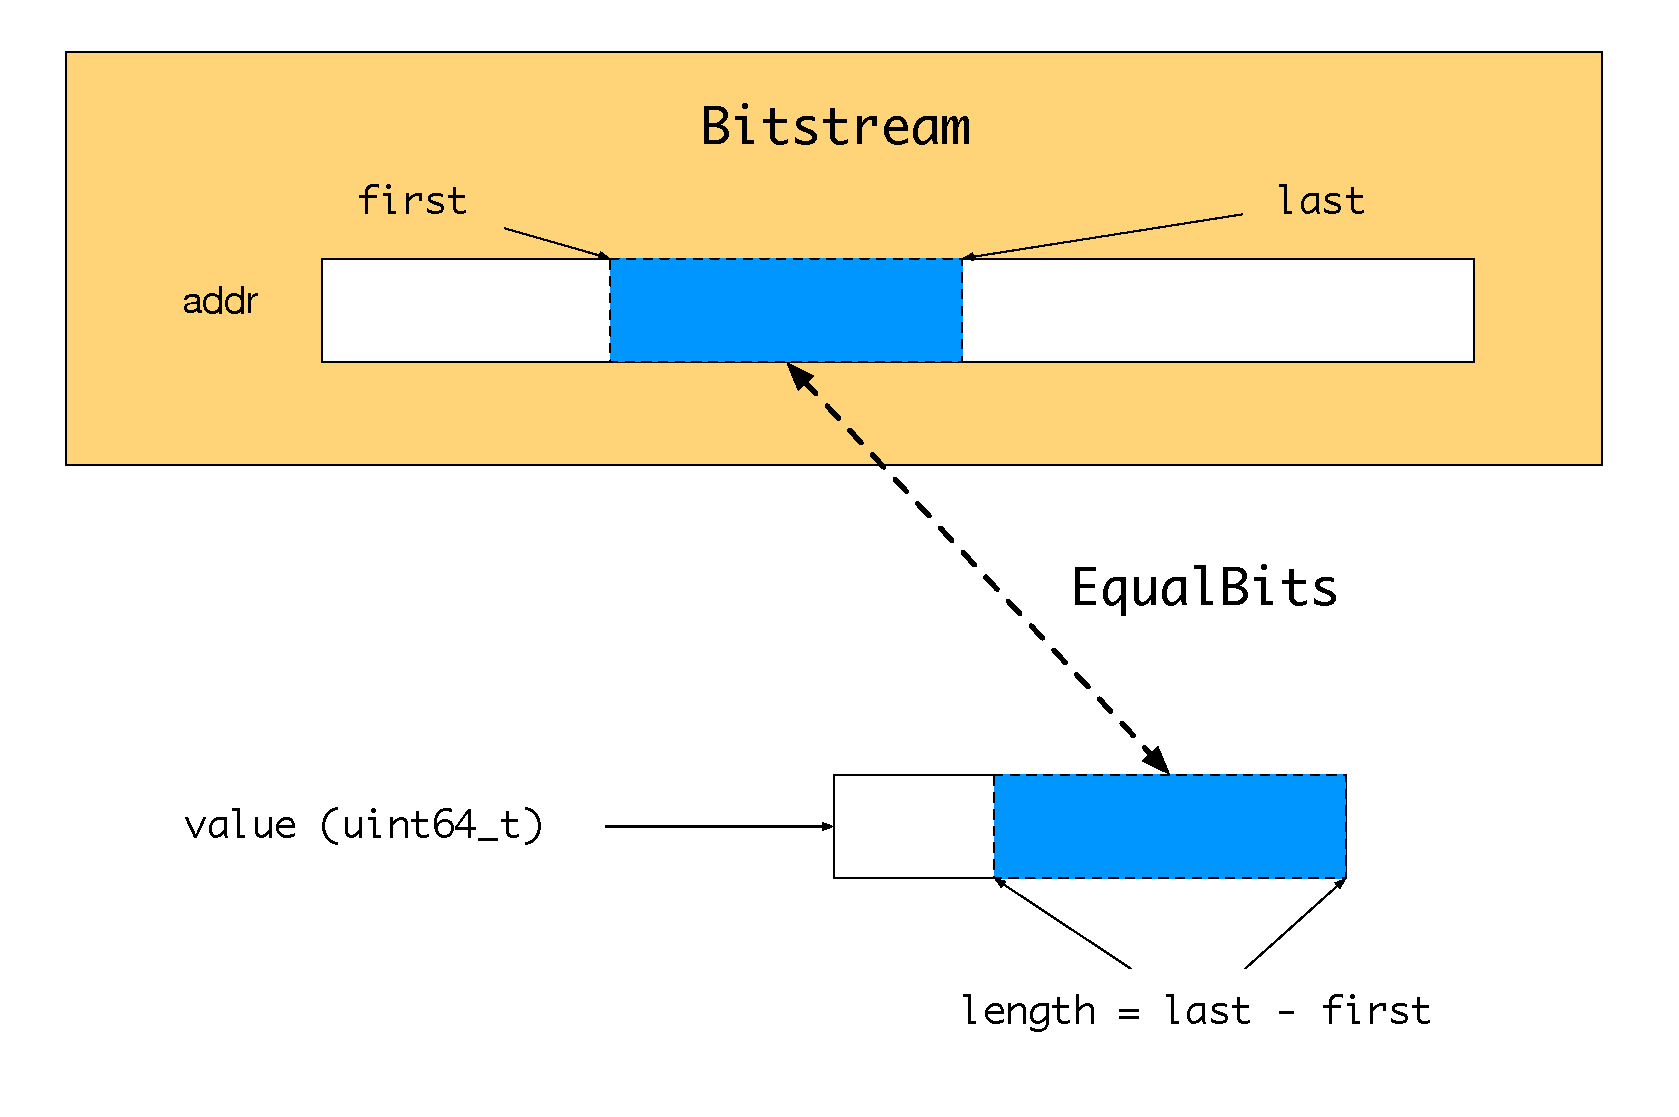
\includegraphics[width=0.99\textwidth]{figures/equalbits.pdf}
\caption{\label{fig:EqualBits correspondance}
	Bit coincidences required by \inl{EqualBits}}
\end{center}
\end{figure}



\section{Auxiliary \inl{Bitstream} functions}
\label{sec:bitstream-aux}


As a kind of constructor for type
\inl{Bitstream}, we provide the operation \inl{Bitstream_Init},
shown with its contract in Listing~\ref{lst:Bitstream_Init}.




\begin{listing}[hbt]
\begin{minipage}{0.99\textwidth}
\begin{lstlisting}[style=acsl-block]
/*@
  requires valid:     Writeable(stream);
  requires bit_size:  8 * size <= UINT32_MAX;
  requires valid_pos: bitpos <= 8 * size;
  requires separated: \separated(addr + (0..size-1), stream);

  assigns  stream->addr, stream->size, stream->bitpos;

  ensures  addr:      stream->addr == addr;
  ensures  size:      stream->size == size;
  ensures  bitpos:    stream->bitpos == bitpos;
  ensures  invariant: Invariant(stream, 0);
*/
void Bitstream_Init(Bitstream* stream, uint8_t* addr, uint32_t size, uint32_t bitpos);
\end{lstlisting}
\end{minipage}
\caption{\label{lst:Bitstream_Init}Setting-up a bitstream}
\end{listing}

\FloatBarrier

Moreover, we provide a test for exhaustion of a \inl{Bitstream},
shown in Listing~\ref{lst:Bitstream_Normal}.


\begin{listing}[hbt]
\begin{minipage}{0.99\textwidth}
\begin{lstlisting}[style=acsl-block]
/*@
  requires valid:     Readable(stream);
  requires invariant: Invariant(stream, length);

  assigns \nothing;

  ensures  result:    \result <==> Normal(stream, length);
*/
int Bitstream_Normal(const Bitstream* stream, uint32_t length);
\end{lstlisting}
\end{minipage}
\caption{\label{lst:Bitstream_Normal}Testing a bitstream for exhaustion}
\end{listing}



\FloatBarrier


\section{Writing bit sequences}
\label{sec:writing bit sequences}

In this section, we describe the operations that handle plain bit sequences.
%
They are used to implement the \inl{Bitstream} operations for
Section~\ref{sec:bitstream}.

Listing~\ref{lst:Bitstream_Write impl} shows contract of
the \inl{Bitstream_Write} operation,
and moreover exemplifies its implementation.


\begin{listing}[hbt]
\begin{minipage}{0.99\textwidth}
\begin{lstlisting}[style=acsl-block]
/*@
  requires valid:      Writeable(stream);
  requires invariant:  Invariant(stream, length);
  requires normal:     Normal(stream, length);
  requires upper:      UpperBitsNotSet(value, length);

  assigns stream->addr[0..stream->size - 1];
  assigns stream->bitpos;

  ensures  pos:        stream->bitpos == \old(stream->bitpos) + length;
  ensures  changed:    EqualBits(stream, \old(stream->bitpos), stream->bitpos, value);
  ensures  unchanged:  Unchanged{Here,Old}(stream, 0, \old(stream->bitpos));
  ensures  unchanged:  Unchanged{Here,Old}(stream, stream->bitpos, 8 * stream->size);
  ensures  size:       stream->size == \old(stream->size);
*/
void Bitstream_Write(Bitstream* stream, uint32_t length, uint64_t value)
{
    Bitwalker_Write(stream->addr, stream->size, stream->bitpos, length, value);
    //@ assert EqualBits(stream, stream->bitpos, stream->bitpos + length, value);

    stream->bitpos += length;
    //@ assert EqualBits(stream, \at(stream->bitpos,Pre), stream->bitpos, value);
}

\end{lstlisting}
\end{minipage}
\caption{\label{lst:Bitstream_Write impl}Writing to a bitstream}
\end{listing}

\FloatBarrier

Most parts of the contract are quite similar to that of
\inl{Bitstream_Read} in
Listing~\ref{lst:Bitstream_Read spec}.
%
Differences are the following:
\begin{itemize}
\item We require that the \inl{value} to be written fits into
	the specified
	\inl{length}, i.e.\ its unused most significant bits
	are zero (requirement property
	``\inl{upper}'').
\item The operation is allowed to change the contents of the bitstream
	(first \inl{assigns} clause) in addition to the streams
	current bit
	position (second \inl{assigns} clause), but no other
	memory locations.
\item Since we couldn't specify in the \inl{assigns} clauses 
	which bits exactly are allowed to be modified, we give the
	details in two
	\inl{ensures} clauses named ``\inl{unchanged}'':
	All bits before the stream's \inl{bitpos} on operation
	entry, and after
	its \inl{bitpos} on exit, must remain unchanged.
\end{itemize}

The implementation just employs the lower-level operation
\inl{Bitwalker_Write} to
write the bits, and appropriately updates the \inl{stream}'s
\inl{bitpos}.
%
Two assertions were needed to help the provers establishing that
\inl{value}'s
bits are actually written to \inl{stream}'s data array by

\fxfatal{something is missing here!!}


The formal definitions of the used \acsl predicates are given in
Listing~\ref{lst:Bitsequence preds}.
%
Again, the tacit assumption that the array contains sensible data
up to its very last bit is used in predicate \inl{Normal}.



\begin{listing}[hbt]
\begin{minipage}{0.99\textwidth}
\begin{lstlisting}[style=acsl-block]
/*@
   predicate Readable{L}(uint8_t* addr, integer size) = \valid_read(addr + (0..size-1));

   predicate Writeable{L}(uint8_t* addr, integer size) = \valid(addr + (0..size-1));

   predicate Invariant{L}(integer size, integer bitpos, integer length) =
       8 * size <= UINT32_MAX         &&
       length <= 64                   &&
       bitpos + length <= UINT32_MAX;

    predicate Normal{L}(integer size, integer bitpos, integer length) =
       bitpos + length <= 8 * size;
*/
\end{lstlisting}
\end{minipage}
\caption{\label{lst:Bitsequence preds} \acsl predicates used in bit sequence layer contracts}
\end{listing}


\FloatBarrier


Listing~\ref{Bitwalker_Write spec} shows the contract, and the
implementation, of the
\inl{Bitwalker_Write} operation.

\begin{listing}[hbt]
\begin{minipage}{0.99\textwidth}
\begin{lstlisting}[style=acsl-block]
/*@
  requires valid:      Writeable(addr, size);
  requires invariant:  Invariant(size, bitpos, length);
  requires normal:     Normal(size, bitpos, length);
  requires upper:      UpperBitsNotSet(value, length);

  assigns addr[0..size-1];

  ensures  left:       Unchanged{Here,Old}(addr, 0, bitpos);
  ensures  middle:     EqualBits(addr, bitpos, bitpos + length, value);
  ensures  right:      Unchanged{Here,Old}(addr, bitpos + length, 8 * size);
*/
void Bitwalker_Write(uint8_t* addr, uint32_t size, uint32_t bitpos, uint32_t length, uint64_t value);
{
    /*@
      loop invariant bound:   bitpos <= i <= bitpos + length;
      loop invariant left:    Unchanged{Here,Pre}(addr, 0, bitpos);
      loop invariant middle:  EqualBits(addr, bitpos, i, value, length);
      loop invariant right:   Unchanged{Here,Pre}(addr, i, 8 * size);

      loop assigns  i, addr[0..size-1];
      loop variant  bitpos + length - i;
    */
    for (uint32_t i = bitpos; i < bitpos + length; ++i)
    {
        int flag = TestBit64(value, (64 - length) + (i - bitpos));
        SetBit8Array(addr, size, i, flag);
    }   
}

\end{lstlisting}
\end{minipage}
\caption{\label{Bitwalker_Write spec}Writing a bit sequence}
\end{listing}

\FloatBarrier

\section{Reading bit sequences}
\label{sec:reading bit sequences}

The following peculiarities are observed when the former is
compared to \inl{Bitwalker_Read}'s contract in Listing~\ref{lst:Bitwalker_Read spec}.

\begin{listing}[hbt]
\begin{minipage}{0.99\textwidth}
\begin{lstlisting}[style=acsl-block]
/*@
  requires  valid:      Readable(addr, size);
  requires  invariant:  Invariant(size, bitpos, length);
  requires  normal:     Normal(size, bitpos, length);

  assigns   \nothing;

  ensures   equal:      EqualBits(addr, bitpos, bitpos + length, \result);
  ensures   upper:      UpperBitsNotSet(\result, length);
*/
uint64_t Bitwalker_Read(uint8_t* addr, uint32_t size, uint32_t bitpos, uint32_t length);
\end{lstlisting}
\end{minipage}
\caption{\label{lst:Bitwalker_Read spec}Reading a bit sequence}
\end{listing}

\FloatBarrier

\begin{itemize}
\item We require that the \inl{value} to be written fits into
the specific
	\inl{length}, i.e.\ all but its \inl{length}
	least significant bits are
	zero (requirement property ``\inl{upper}'').
\item The operation may modify the data array at \inl{addr},
but nothing else.
\item Again, we give the details of which data bits exactly
	are allowed to be changed in two
	\inl{ensures} clauses, named ``\inl{left}'' and
	``\inl{right}'', and requiring all bits before
	\inl{bitpos} and after
	\inl{bitpos+length} to remain unchanged, respectively.
\end{itemize}

In the implementation, which is shown here as an example, we used
the straight-forward
algorithm that takes a bit from \inl{value} and places it into
the \inl{addr} array, bit by bit.
%
In order for the provers to establish that algorithm's correctness,
we had to provide a total of six \acsl clauses about the loop:
%
\begin{itemize}
\item The loop variable, \inl{i}, always ranges in the interval
	[\inl{bitpos}\ldots\inl{bitpos+length}]---loop invariant property ``\inl{bound}''.
	%
	Note that the highest value is actually taken,
	viz.\ on exit of the loop body in the last iteration,
	subsequently causing the loop to terminate.
\item The bits before \inl{bitpos}, and after
	\inl{bitpos+length}
	remain as they were on operation entry---invariant property
	``\inl{left}'' and ``\inl{right}'', respectively.
\item In the \inl{i}th iteration, the bits
	[\inl{bitpos}\ldots\inl{bitpos+i}) agree with
	the least significant
	\inl{i} bits of \inl{value}---invariant property
	``\inl{middle}''.
\item The loop code is allowed to modify the variable \inl{i},
	and the whole array
	at \inl{addr}, but nothing else---
	\inl{loop assigns} clause.
\item The value of the integer
	expression \inl{bitpos+length-i} is non-negative throughout
	the whole loop execution, but is decreased in every iteration 
	--- \inl{loop variant} clause.
	%
	Therefore, the loop is guaranteed to terminate eventually.
\end{itemize}




The operations we have discussed here are based
on operations to write and to read a single bit.
%
The details of the latter, as well as of the predicates used in their
contracts, are given in Appendix~\ref{cha:low-level bitstream}.


\section{Verification of the Bitstream abstraction}
\label{sec:bitstream verif}



Critics of the formal software verification approach often 
argue that verifying an operation against its formal specification
results in little or no increase of trustworthiness when
%
\begin{itemize}
\item the specification, including all auxiliary definitions etc., is
	as complex as the operation's implementation, or/and
\item the specification essentially duplicates the implemented
	algorithm in a different (such as functional rather than
	imperative) language.
\end{itemize}
%
Both criteria may be seen to be met by our Bitwalker case study.



However, since the operations we dealt with essentially implement a
communication protocol, there is a very simple ``high-level'' property
that should be satisfied, viz.\ that a ``send'' operation is inverse
to a ``receive'' operation.
%
This property can be stated formally in a very brief and understandable
way.
%
It ensures, in a mathematical context, that both operations implement
bijective mappings, that is, in an engineering sense, that the
communication channel neither looses, nor subjoins information.
%
In fact, we have achieved to formally prove this property.




More particularly, in our setting, we could show that the operations
\inl{Bitstream_Read} and \inl{Bitstream_Write} are
inverse to each other.
%
To this end, we set up two fictitious \isoc procedures realizing
the composition of both operations in the two possible orders.




Listing~\ref{lst:Bitstream_WriteThenRead}
shows the procedure for the scenario ``use \inl{Bitstream_Write}
to write a value to a stream, then immediately read it back using
\inl{Bitstream_Read}''.


\begin{listing}[hbt]
\begin{minipage}{0.99\textwidth}
\begin{lstlisting}[style=acsl-block]
/*@
    requires valid:      Writeable(stream);
    requires invariant:  Invariant(stream, length);
    requires normal:     Normal(stream, length);
    requires upper:      UpperBitsNotSet(value, length);

    assigns stream->addr[0..stream->size-1];
    assigns stream->bitpos;

    ensures equality:     \result == value;
*/
uint64_t Bitstream_WriteThenRead(Bitstream* stream, uint32_t length, uint64_t v>
{
    //@ ghost uint32_t old_pos = stream->bitpos;

    Bitstream_Write(stream, length, value);
    //@ assert equal:  EqualBits(stream, old_pos, old_pos+length, value);

    /*@ 
        assigns stream->bitpos;
        ensures reset: stream->bitpos == \at(stream->bitpos,Pre);
    */
    stream->bitpos -= length;

    uint64_t result = Bitstream_Read(stream, length);
    //@ ghost uint32_t new_pos = stream->bitpos;
    //@ assert equal_result: EqualBits(stream, old_pos, new_pos, result);
    //@ assert equal_value:  EqualBits(stream, old_pos, new_pos, value);
    /*@ assert aux:          \forall integer k; old_pos <= k < new_pos ==>
                               \let j = new_pos - 1 - k;
                               (BitTest(value,  j) <==> BitTest(result, j));
    */
    //@ assert left:         EqualBits64(result, value, 64-length, 64);
    //@ assert compare:      EqualBits64(result, value, 0, 64);

    return result;
}
\end{lstlisting}
\end{minipage}
\caption{\label{lst:Bitstream_WriteThenRead}
	Verifying the scenario ``write, then read'' }
\end{listing}

\FloatBarrier

The procedure's body code is straightforward; after
\inl{Bitstream_Write}, we have to seek back to the original bit
position, before calling \inl{Bitstream_Read}''.
%
We could show that the read value always equals the written one,
provided
\begin{itemize}
\item the stream is accessible for both read and update
	(requirement property ``\inl{valid}''),
\item it satisfies its type invariant (property
	``\inl{invariant}''; cf.\ Listing~\ref{lst:Bitstream preds}
	and~\ref{lst:Bitsequence preds}),
\item the stream's current bit position is sufficiently small such that
	all value bits still fit into the stream
	(property``\inl{normal}''), and
\item the most significant value bits that are not written are all zero
	(property``\inl{upper}'').
\end{itemize}
%
This ensures that the bitstream communication channel doesn't loose
information---every value we write into it can completely be
restored.



Vice versa, we could also show that the channel doesn't transmit more
information than is needed to fulfill its task.
%
Listing~\ref{lst:Bitstream_ReadThenWrite}
shows the procedure for the scenario ``use \inl{Bitstream_Read}
to read a value from a stream, then immediately write it back using
\inl{Bitstream_Write}''.




\begin{listing}[hbt]
\begin{minipage}{0.99\textwidth}
\begin{lstlisting}[style=acsl-block]
/*@
    requires valid:      Writeable(stream);
    requires invariant:  Invariant(stream, length);
    requires normal:     Normal(stream, length);

    assigns stream->addr[0..stream->size-1];
    assigns stream->bitpos;

    ensures  unchanged:  Unchanged{Here,Old}(stream, 0, 8 * stream->size);
*/
void Bitstream_ReadThenWrite(Bitstream* stream, uint32_t length)
{
    //@ ghost uint32_t old_pos = stream->bitpos;
    uint64_t value = Bitstream_Read(stream, length);
    //@ assert equal:  EqualBits(stream, old_pos, old_pos+length, value);

    stream->bitpos -= length;
    //@ assert stream->bitpos == old_pos;

    Bitstream_Write(stream, length, value);
    //@ assert unchanged:  Unchanged{Here,Pre}(stream, old_pos, stream->bitpos);
}
\end{lstlisting}
\end{minipage}
\caption{\label{lst:Bitstream_ReadThenWrite}
	Verifying the scenario ``read, then write'' }
\end{listing}


\FloatBarrier


We were able show that this leaves the
whole stream unchanged, provided the first three requirement properties
from \inl{Bitstream_WriteThenRead} are met.
%
As an example for a channel transmitting redundant information,
consider
a bitstream implementation
with \inl{Bitstream_Write}
storing each byte twice in succession and \inl{Bitstream_Read}
ignoring every second byte.
%
Such a stream doesn't meet our property, since, 
starting from a stream with non-agreeing adjacent bytes, there is no
way to reproduce it by a ``read, then write'' scenario.
\cleardoublepage
%
\chapter{Formal verification}
\label{cha:formal-verification}

\section{Bit stream and lower-level bit operations}
\label{sec:bitstream-verification}

\begin{table}[hbt]
\begin{center}
    \begin{tabular}{|l|ccc|cccc|}
\hline
\multirow{2}{*}{\textbf{component}} &
\multicolumn{3}{c|}{ \textbf{vcs}} &
\multicolumn{4}{c|}{\textbf{individual provers}}\\
\cline{2-8}
               &  all & proven & (\%) & qed & alt-ergo & cvc4 & z3  \\
\hline
\hline
bit stream     & 58 &  58 & 100 & 19 &  0 & 0 & 39  \\
\hline
bit stream (inverse)  & 58 & 58 & 100 & 33 &  2 & 1 & 22  \\
\hline
lower-level bit ops & 126 & 126 & 100 & 55 &  0 & 1 & 70  \\
\hline
\end{tabular}
\end{center}
\caption{\label{tbl:bitstream-verification} verfication result for bit stream and lower-level bit operations}
\end{table}

\FloatBarrier  % forces the output of listings/tables

\section{Verification of packets without \inl{N_ITER}}
\label{sec:packets-without-niter-verification}


\begin{table}[hbt]
\begin{center}
    \begin{tabular}{|m{10ex}|m{5ex}m{5ex}m{5ex}|m{5ex}m{5ex}m{5ex}m{5ex}|}
\hline
\multirow{2}{*}{\textbf{PacketID}} &
\multicolumn{3}{c|}{ \textbf{VCs}} &
\multicolumn{4}{c|}{\textbf{Individual Provers}}\\
\cline{2-8}
               &  All & Proven & (\%) & Qed & Alt-Ergo & CVC4 & Z3  \\
\hline
\hline
16 & 436 & 436 & 100 & 318 & 0 & 1 & 117\\
\hline
39 & 483 & 483 & 100 & 346 & 0 & 1 & 136\\
\hline
42 & 559 & 543 & 97 & 399 & 0 & 1 & 143\\
\hline
45 & 389 & 389 & 100 & 290 & 0 & 1 & 98\\
\hline
57 & 483 & 483 & 100 & 346 & 0 & 1 & 136\\
\hline
65 & 624 & 624 & 100 & 430 & 0 & 1 & 193\\
\hline
66 & 389 & 389 & 100 & 290 & 0 & 1 & 98\\
\hline
71 & 530 & 530 & 100 & 374 & 0 & 1 & 155\\
\hline
72 & 999 & 957 & 95 & 671 & 0 & 1 & 285\\
\hline
76 & 958 & 938 & 97 & 644 & 9 & 1 & 284\\
\hline
90 & 474 & 465 & 98 & 341 & 0 & 1 & 123\\
\hline
\end{tabular}
\end{center}
\caption{\label{tbl:packets-without-niter-tracktotrain-part1} Verfication result for TrackToTrain packets without \inl{N_ITER} part 1}
\end{table}

\FloatBarrier  % forces the output of listings/tables

\begin{table}[hbt]
\begin{center}
    \begin{tabular}{|m{10ex}|m{5ex}m{5ex}m{5ex}|m{5ex}m{5ex}m{5ex}m{5ex}|}
\hline
\multirow{2}{*}{\textbf{PacketID}} &
\multicolumn{3}{c|}{ \textbf{VCs}} &
\multicolumn{4}{c|}{\textbf{Individual Provers}}\\
\cline{2-8}
               &  All & Proven & (\%) & Qed & Alt-Ergo & CVC4 & Z3  \\
\hline
\hline
131 & 624 & 624 & 100 & 430 & 0 & 1 & 193\\
\hline
132 & 389 & 389 & 100 & 290 & 0 & 1 & 98\\
\hline
133 & 718 & 718 & 100 & 486 & 0 & 1 & 231\\
\hline
134 & 624 & 624 & 100 & 430 & 0 & 1 & 193\\
\hline
136 & 474 & 465 & 98 & 341 & 0 & 1 & 123\\
\hline
137 & 389 & 389 & 100 & 290 & 0 & 1 & 98\\
\hline
138 & 483 & 483 & 100 & 346 & 0 & 1 & 136\\
\hline
139 & 483 & 483 & 100 & 346 & 0 & 1 & 136\\
\hline
140 & 389 & 389 & 100 & 290 &  0 &  1 & 98\\
\hline
141 & 436 & 436 & 100 & 318 & 0 & 1 & 117\\
\hline
254 & 342 & 342 & 100 &262 & 0 & 1 & 79\\
\hline
\end{tabular}
\end{center}
\caption{\label{tbl:packets-without-niter-tracktotrain-part2} Verfication result for TrackToTrain packets without \inl{N_ITER} part 2}
\end{table}

\FloatBarrier  % forces the output of listings/tables

\begin{table}[hbt]
\begin{center}
    \begin{tabular}{|m{10ex}|m{5ex}m{5ex}m{5ex}|m{5ex}m{5ex}m{5ex}m{5ex}|}
\hline
\multirow{2}{*}{\textbf{PacketID}} &
\multicolumn{3}{c|}{ \textbf{VCs}} &
\multicolumn{4}{c|}{\textbf{Individual Provers}}\\
\cline{2-8}
               &  All & Proven & (\%) & Qed & Alt-Ergo & CVC4 & Z3  \\
\hline
\hline
1 & 973 & 948 & 97 & 649 & 6 & 2 & 291\\
\hline
4 & 342 & 342 & 100 & 262 & 0 & 1 & 79\\
\hline
9 & 342 & 342 & 100 & 262 & 0 & 1 & 79\\
\hline
44 & 389 & 389 & 100 & 290 & 0 & 1 & 98\\
\hline
\end{tabular}
\end{center}
\caption{\label{tbl:packets-without-niter-traintotrack} Verfication result for TrainToTrack packets without \inl{N_ITER}}
\end{table}

\FloatBarrier  % forces the output of listings/tables

\begin{table}[hbt]
\begin{center}
    \begin{tabular}{|m{10ex}|m{5ex}m{5ex}m{5ex}|m{5ex}m{5ex}m{5ex}m{5ex}|}
\hline
\multirow{2}{*}{\textbf{PacketID}} &
\multicolumn{3}{c|}{ \textbf{VCs}} &
\multicolumn{4}{c|}{\textbf{Individual Provers}}\\
\cline{2-8}
               &  All & Proven & (\%) & Qed & Alt-Ergo & CVC4 & Z3  \\
\hline
\hline
255 & 239 & 239 & 100 & 192 & 0 & 1 & 46\\
\hline
\end{tabular}
\end{center}
\caption{\label{tbl:packets-without-niter-bothways} Verfication result for BothWays packets without \inl{N_ITER}}
\end{table}

\FloatBarrier  % forces the output of listings/tables

\begin{table}[hbt]
\begin{center}
    \begin{tabular}{|m{8ex}|m{11cm}|m{9ex}|m{11ex}|}
\hline
               PacketID & Packetname & \inl{N_ITER} & Conditionals\\
\hline
\hline
3 & \inl{NationalValues} & dynamic & conditional\\
\hline
5 & \inl{Linking} & dynamic & conditional\\
\hline
12 & \inl{Level1MovementAuthority} & dynamic & -\\
\hline
15 & \inl{Level23MovementAuthority} & dynamic & -\\
\hline
16 & \inl{RepositioningInformation} & static & -\\
\hline
21 & \inl{GradientProfile} & dynamic & -\\
\hline
27 & \inl{InternationalStaticSpeedProfile} & dynamic & -\\
\hline
39 & \inl{TrackConditionChangeOfTractionPower} & static & -\\
\hline
41 & \inl{LevelTransitionOrder} & dynamic & conditional\\
\hline
42 & \inl{SessionManagement} & static & conditional\\
\hline
45 & \inl{RadioNetworkRegistration} & static & -\\
\hline
46 & \inl{ConditionalLevelTransitionOrder} & dynamic & conditional\\
\hline
49 & \inl{ListOfBalisesForSHArea} & dynamic & conditional\\
\hline
51 & \inl{AxleLoadSpeedProfile} & dynamic & -\\
\hline
57 & \inl{MovementAuthorityRequestParameters} & static & -\\
\hline
58 & \inl{PositionReportParameters} & dynamic & -\\
\hline
63 & \inl{ListOfBalisesInSRAuthority} & dynamic & conditional\\
\hline
65 & \inl{TemporarySpeedRestriction} & static & -\\
\hline
66 & \inl{TemporarySpeedRestrictionRevocation} & static & -\\
\hline
67 & \inl{TrackConditionBigMetalMasses} & dynamic & -\\
\hline
68 & \inl{TrackCondition} & dynamic & conditional\\
\hline
\end{tabular}
\end{center}
\caption{\label{tbl:packets-packetnumbers-tracktotrain-part1} TrackToTrain packets part 1}
\end{table}


\FloatBarrier  % forces the output of listings/tables

\begin{table}[hbt]
\begin{center}
    \begin{tabular}{|m{8ex}|m{11cm}|m{9ex}|m{11ex}|}
\hline
               PacketID & Packetname & \inl{N_ITER} & Conditionals\\
\hline
\hline
70 & \inl{RouteSuitabilityData} & dynamic & conditional\\
\hline
71 & \inl{AdhesionFactor} & static & -\\
\hline
72 & \inl{PacketForSendingPlainTextMessages} & static & conditional\\
\hline
76 & \inl{PacketForSendingFixedTextMessages} & static & conditional\\
\hline
79 & \inl{GeographicalPositionInformation} & dynamic & conditional\\
\hline
80 & \inl{ModeProfile} & dynamic & -\\
\hline
90 & \inl{TrackAheadFreeUpToLevel23TransitionLocation} & static & conditional \\
\hline
131 & \inl{RBCTransitionOrder} & static & -\\
\hline
132 & \inl{DangerForShuntingInformation} & static & -\\
\hline
133 & \inl{RadioInfillAreaInformation} & static & -\\
\hline
134 & \inl{EOLMPacket} & static & -\\
\hline
136 & \inl{InfillLocationReference} & static & conditional\\
\hline
137 & \inl{StopIfInStaffResponsible} & static & -\\
\hline
138 & \inl{ReversingAreaInformation} & static & -\\
\hline
139 & \inl{ReversingSupervisionInformation} & static & -\\
\hline
140 & \inl{TrainRunningNumberFromRBC} & static & -\\
\hline
141 & \inl{DefaultGradientForTemporarySpeedRestriction} & static & -\\
\hline
254 & \inl{DefaultBaliseLoopOrRIUInformation} & static & -\\
\hline
\end{tabular}
\end{center}
\caption{\label{tbl:packets-packetnumbers-tracktotrain-part2} TrackToTrain packets part 2}
\end{table}

\FloatBarrier  % forces the output of listings/tables

\begin{table}[hbt]
\begin{center}
    \begin{tabular}{|m{8ex}|m{11cm}|m{9ex}|m{11ex}|}
\hline
               PacketID & Packetname & \inl{N_ITER} & Conditionals \\
\hline
\hline
1 & \inl{PositionReportBasedOnTwoBaliseGroups} & static & conditional\\
\hline
3 & \inl{OnboardTelephoneNumbers} & dynamic & -\\
\hline
4 & \inl{ErrorReporting} & static & -\\
\hline
9 & \inl{Level23TransitionInformation} & static & -\\
\hline
11 & \inl{ValidatedTrainData} & dynamic & -\\
\hline
44 & \inl{DataUsedByApplicationsOutsideTheERTMSETCSSystem} & static & -\\
\hline
\end{tabular}
\end{center}
\caption{\label{tbl:packets-packetnumbers-traintotrack} TrainToTrack packets}
\end{table}

\FloatBarrier  % forces the output of listings/tables

\begin{table}[hbt]
\begin{center}
    \begin{tabular}{|m{8ex}|m{11cm}|m{9ex}|m{11ex}|}
\hline
               PacketID & Packetname & \inl{N_ITER} & Conditionals \\
\hline
\hline
255 & \inl{EndOfInformation} & static & -\\
\hline
\end{tabular}
\end{center}
\caption{\label{tbl:packets-packetnumbers-bothways} BothWays packets}
\end{table}

\FloatBarrier  % forces the output of listings/tables

\cleardoublepage
%
\chapter{Static Analysis of Bitwalker}
\label{sec:static-analysis}

\section{Introduction}
In this chapter we describe our work on the static code analysis of the bitwalker code provided in \href{https://github.com/openETCS/validation/tree/master/Artifacts/Subset-026-7_XML/Subset026_7/Bitwalker}{[validation repository]}

Our aim is to discover programing errors, obtain code metrics (lines of code, lines of code/lines of comments, cyclomatic complexity, Halsted metrics, class inherance tree and others) and verify the C11 standard and some subset of rules defined in the MISRA C Standard. That is, we focus on the different aspects of the source code to ensure the quality of the code in various perspectives.

The code metrics help understanding the complexity of the code and can lead to code changes. The complexity metrics allows us to identify particularly complex program areas that it would be desirable to redesign, and where problems that will appear in the maintenance phase are likely focused. For example, the cyclomatic complexity or the number of paths, is a software quality metric that quantifies the complexity of a program and also indicates the number of test cases that would have to be written to execute all paths in a program. However, the cyclomatic complexity only considers the decision structure of a program, not consider the complexity of nesting. There are more complexity metrics that takes into account the degree of nesting of a program or that consider the volumen and the program level like the Halsted metrics. The conjunction of the complexity metrics are an important indicator of the code readability, maintainability and portability, and the more complex the code is, more likely it will contain masked bugs.

CENELEC Standard identifies techniques and measures for 5 levels of software safety integrity and requires the use of a package of techniques and their correct
application appropriate to the software safety integrity level.

Six different static analysis tools have been used during the code verification activities in order to assess the quality of the results, ensure code quality and cover different techniques and metrics high recommended by CENELEC Standard. The selected tools are:
\begin{itemize}
\item \textbf{Resource Standard Metrics (\href{http://msquaredtechnologies.com/m2rsm/}{RSM})}: a source code metrics and quality analysis tool
\item \textbf{\href{http://www.locmetrics.com/}{LocMetrics}}: a simple tool for counting lines of code in C\#, Java, and C++
\item \textbf{\href{http://www.scitools.com/}{Understand}}: a reverse engineering, documentation and metrics tool for C and C++ source code. It offers code navigation using a detailed cross reference, a syntax colorizing "smart" editor, and a variety of graphical reverse engineering views.                          
\item \textbf{\href{http://clang-analyzer.llvm.org/}{Clang Static Analyzer}}: The Clang Static Analyzer consists of both a source code analysis framework and a standalone tool that finds bugs in C and Objective-C programs.
\item \textbf{\href{http://cppcheck.sourceforge.net/}{CPPcheck}}: a static analysis tool for C, C++ code. Unlike C, C++ compilers and many other analysis tools it does not detect syntax errors in the code. Cppcheck primarily detects the types of bugs that the compilers normally do not detect. 
\item \textbf{\href{http://www.verifysoft.com/en_cmtx.html}{Testwell CMT++}}: Based on the static properties of the program code CMT++ gives estimates how error prone the program source code is due to its complexity, how long it will take to understand the code, what is the logical volume of the code, etc ...
\end{itemize}


Finally, according to the results obtained by using the tools, we will present some conclusions.

\section{Resource Standard Metrics -RSM- Results}
In this section we provide the results obtained with the \href{http://msquaredtechnologies.com/m2rsm/}{[RSM]} tool.

Resource Standard Metrics (RSM) is a source code metrics and quality analysis tool. This tool provides standard metrics and a combination of features that allow to:
\begin{itemize}
\item Analyze source code for programming errors
\item Analyze source code for code style enforcement
\item Create an Inheritance tree from the code
\item Collect Source Code Metrics by the function, class, file, and project
\item Analyze Cyclomatic Complexity
\end{itemize}

Besides, RSM has intrinsic quality notices, can be extended by the end user with User Defined Quality Notices using regular expressions to analyze code lines and it is mapped to the MISRA C Standard. 

RSM has been customized to obtain the below metrics and analysis and the corresponding reports that are available into the \href{https://github.com/openETCS/validation/tree/master/VnVUserStories/VnVUserStorySQS/04-Results}{[VnVUserStories folder]}

\begin{itemize}
\item Project Functional Metrics and Analysis
\item Project Class/Struct Metrics and Analysis
\item Class Inheritance Tree
\item Project Quality Profile
\item Quality Notice Density
\item Files Keywords and Metrics
\item Project Keywords and Metrics
\item Files Function Metrics
\item Class/Struct Metrics
\item Complexity Metrics
\end{itemize}

As mentioned previously CENELEC Standard requires the use of a package of techniques. With the use of the RSM tool the following Cenelec Standard techniques have been covered:
\begin{itemize}
\item Limited Size and Complexity in Functions, Subroutines and Methods (High Recommended)
\item Coding Standard (Mandatory): At this point the fulfillment of some of the MISRA-C Standard rules has been checked.
\end{itemize}

\subsection{Quality Metrics}

As well as having intrinsic and user definied quality notices, RSM tool is mapped to the MISRA C Industry Standard. Taking into account the intrisic quality notice and the user defined quality notices the RSM tool covers 40.16\% of \href{http://msquaredtechnologies.com/m2rsm/docs/QualityStandards/MISRA_C_Mapping.htm}{[MISRA C]} rules.

The following table shows the intrinsic Quality Notices for C language that RSM tool checks.

{\footnotesize\sffamily\centering
  \begin{longtable}{||p{.45\textwidth}|p{.5\textwidth}||}
  \caption{Quality Notices}\\
    \hline\hline
    \hline\hline
    \endhead
    \hline\hline
    \endfoot
    \textbf{Quality Notice No. 1}

Emit a quality notice when the physical line length is greater than the specified number of characters.

Rationale:  \textcolor{red}{Reproducing source code on devices that are limited to 80 columns of text can cause the truncation of the line or wrap the line.  Wrapped source lines are difficult to read, thus creating weaker peer reviews of the source code}.
& \textbf{Quality Notice No. 2}

Emit a quality notice when the function name length is greater than the specified number of characters.  

Rationale:  \textcolor{red}{Long function names may be a portability issue especially when code has to be cross compiled onto embedded platforms.  This difficultly is typically seen with older hardware and operating systems.}
    \\
    \hline \textbf{Quality Notice No. 3}
    
Emit a quality notice when ellipsis '...' are identified within a functions parameter list thus enabling variable arguments.  

Rationale:  \textcolor{red}{Ellipsis create a variable argument list.  This type of design is found in C and C++.  It essentially breaks the type strict nature of C++ and should be avoided.}
 & \textbf{Quality Notice No. 4}
 
Emit a quality notice if there exists an assignment
operator '=' within a logical 'if' condition.

Rationale:  \textcolor{red}{An assignment within an "if" condition is likely a typographical error giving rise to a logic defect.  However, some programmers place compound statements into the "if" condition making the code difficult to read.}
    \\
    \hline \textbf{Quality Notice No. 5}
    
Emit a quality notice if there exists an assignment
operator '=' within a logical 'while' condition.

Rationale:  \textcolor{red}{An assignment within a "while" condition is likely a typographical error giving rise to a logic defect.  However, some programmers place compound statements into the "while" condition making the code difficult to read.}
 & \textbf{Quality Notice No. 6}
 
Emit a quality notice when a pre-decrement operator '--' is identified within the code.  

Rationale: \textcolor{red}{ The pre-decrement of a variable occurs before the remainder of the processing in the statement.  This can be difficult to comprehend or anticipate.  There are documented cases where the mathematical results vary between the result of macros when different code preprocessors expand the macros into a normal form.  Remember, there is no standard for the preprocessor, just the language.}
    \\
    \hline \textbf{Quality Notice No. 7}
    
Emit a quality notice when a pre-increment operator '++' is identified within the code.

Rationale:  \textcolor{red}{The pre-increment of a variable occurs before the remainder of the processing in the statement.  This can be difficult to comprehend or anticipate.  There are documented cases where the mathematical results vary between the result of macros when different code preprocessors expand the macros into a normal form.}  
& \textbf{Quality Notice No. 8}

Emit a quality notice when the 'realloc' function
is identified within the code.

Rationale:  \textcolor{red}{Using realloc can lead to latent memory leaks within your C or C++ code.  The call to realloc reassigns the pointer to the same memory address using a larger or smaller space.  However if realloc fails, a NULL pointer is returned.  No "free" was performed on the pointer so if you don't retain the pointer before the realloc call, a latent memory leak could occur.}
    \\
    \hline \textbf{Quality Notice No. 9}
    
Emit a quality notice when the 'goto' function
is identified within the code.

Rationale:  \textcolor{red}{The use of "goto" creates spaghetti code.  A "goto" can jump anywhere to the destination label.  This type of design breaks the "one in - one out" ideal of a function creating code which can be impossible to debug or maintain.}
 & \textbf{Quality Notice No. 10}
 
Emit a quality notice when the Non-ANSI function prototype is identified within the code.

Rationale:  \textcolor{red}{Older C code can be written in a style that does not use function prototypes of the function argument types.  This code will not compile on ANSI C and C++ compilers because of this type of weakness.  Identifying this condition can help assess whether code can be ported to a newer version of the language.}
    \\
    \hline \textbf{Quality Notice No. 11}
    
Emit a quality notice when open and closed brackets '[ ]' are not balance within a file.

Rationale:  \textcolor{red}{This type of error is always caught by the compiler as a syntax error.  However, a compiler can be told to ignore source code by using preprocessor directives like \#if ... \#endif.  This is a way to "comment" out large blocks of code.  However, the code still looks like operational code to the maintainer as it is not a comment.  Many hours can be wasted working on dead code.  This quality notice serves to warn you of this dead code that should be removed or converted to actual comment form.}
 & \textbf{Quality Notice No. 12}
 
Emit a quality notice when open and closed parenthesis '( )' are not balance within a file.

Rationale:  \textcolor{red}{This type of error is always caught by the compiler as a syntax error.  However, a compiler can be told to ignore source code by using preprocessor directives like \#if ... \#endif.  This is a way to "comment" out large blocks of code.  However, the code still looks like operational code to the maintainer as it is not a comment.  Many hours can be wasted working on dead code.  This quality notice serves to warn you of this dead code that should be removed or converted to actual comment form.}.
    \\
    \hline \textbf{Quality Notice No. 13}
    
Emit a quality notice when a 'switch' statement does not have a 'default' condition.

Rationale:  \textcolor{red}{A "switch" statement must always have a default condition or this logic construct is non-deterministic.  Generally the default condition should warn the user of an anomalous condition which was not anticipated by the programmer by the case clauses of the switch.}
 & \textbf{Quality Notice No. 14}
 
Emit a quality notice when there are more 'case' conditions than 'break', 'return' or 'fall through' comments.

Rationale:  \textcolor{red}{Many tools, including RSM, watch the use of "case" and "break" to ensure that there is not an inadvertent fall through to the next case statement.  RSM requires the programmer to explicitly indicate in the source code via a "fall through" comment that the case was designed to fall through to the next statement.}
    \\
    \hline \textbf{Quality Notice No. 16}
    
Emit a quality notice when function white space
percentage is less than the specified minimum.

Rationale:  \textcolor{red}{Source code must be easily read.  A low percentage of white space indicates that the source code is crammed together thus compromising the readability of the code.  Typically white space less than 10 percent is considered crammed  code. }
 & \textbf{Quality Notice No. 17}
 
Emit a quality notice when function comment
percentage is less than the specified minimum.

Rationale:  \textcolor{red}{A programmer must supply sufficient comments to enable the understandability of the source code.  Typically a comment percentage less than 10 percent is considered insufficient.  However, the content quality of the comment is just as important as the quantity of the comments.  For this reason you could use the -E option to extract all the comments from a file.  The reviewer should be able to read the comments and extract the story of the code.}
    \\
    \hline \textbf{Quality Notice No. 18}
    
Emit a quality notice when the eLOC within a
function exceeds the specified maximum.

Rationale:  \textcolor{red}{An extremely large function is very difficult to maintain and understand.  When a function exceeds 200 eLOC (effective lines of code), it typically indicates that the function could be broken down into several functions.  Small modules are desirable for modular composability.}
 & \textbf{Quality Notice No. 19}
 
Emit a quality notice when file white space
percentage is less than the specified minimum.

Rationale:  \textcolor{red}{Source code must be easily read.  A low percentage of white space indicates that the source code is crammed together thus compromising the readability of the code.  Typically white space less than 10 percent is considered crammed  code.}

    \\
    \hline \textbf{Quality Notice No. 20}
    
Emit a quality notice when file comment
percentage is less than the specified minimum.

Rationale:  \textcolor{red}{A programmer must supply sufficient comments to enable the understandability of the source code.  Typically a comment percentage less than 10 percent is considered insufficient.  However, the content quality of the comment is just as important as the quantity of the comments.  For this reason you could use the -E option to extract all the comments from a file.  The reviewer should be able to read the comments and extract the story of the code.}
 & \textbf{Quality Notice No. 22}
 
Emit a quality notice when each if, else, for
or while is not bound by scope.

Rationale:  \textcolor{red}{Logical blocks should be bound with scope.  This clearly marks the boundaries of scope for the logical blocks.  Many times, code may be added to non-scoped logic blocks thus pushing other lines of code from the active region of the logical construct giving rise to a logic defect.}
    \\
    \hline 
    \textbf{Quality Notice No. 23}
    
Emit a quality notice when the '?' or the implied
if-then-else construct has been identified.

Rationale:  \textcolor{red}{The ? operator creates the code equivalent of an "if" then "else" construct.  However the resultant source is far less readable.}
 & \textbf{Quality Notice No. 24}
 
Emit a quality notice when an ANSI C++ keyword is identified within a *.c or a *.h file.

Rationale: \textcolor{red}{ In C source code it is possible to find variable names like "class".  This word is a key word in C++ and would prevent this C code from being ported to the C++ language.}
    \\
    \hline
\textbf{Quality Notice No. 25} (Deprecated RSM 6.70) 

When analyzing *.h files for C++ keywords,
assume that *.h can be both C and C++.

Rationale: \textcolor{red}{ A *.h file can be either a C or C++ source file.  If a *.h file is assumed to be from either language, then RSM will not emit C keyword notices in *.h file, only for *.c files.}
 & \textbf{Quality Notice No. 26}
 
Emit a quality notice when a void * is identified
within a source file.

Rationale:  \textcolor{red}{A "void *" is a type-less pointer.  ANSI C and C++ strives to be type strict.  In C++ a "void *" breaks the type strict nature of the language which can give rise to anomalous run-time defects.}
    \\
    \hline
    \textbf{Quality Notice No. 27}
    
Emit a quality notice when the number of function return points is greater than the specified maximum.

Rationale:  \textcolor{red}{A well constructed function has one entry point and one exit point.  Functions with multiple return points are difficult to debug and maintain.}
 & \textbf{Quality Notice No. 28}
 
Emit a quality notice when the cyclomatic complexity of a function exceeds the specified maximum.

Rationale:  \textcolor{red}{Cyclomatic complexity is an indicator for the number of logical branches within a function.  A high degree of V(g), greater than 10 or 20, indicates that the function could be broken down into a more modular design of smaller functions.}
    \\
    \hline
        \textbf{Quality Notice No. 29}
        
Emit a quality notice when the number of function input parameters exceeds the specified maximum.

Rationale:  \textcolor{red}{A high number of input parameters to a function indicates poor modular design.  Data should be grouped into representative data types.  Functions should be specific to one purpose.}
 & \textbf{Quality Notice No. 30}
 
Emit a quality notice when a TAB character is identified within the source code. Indentation with TAB will create editor and device dependent formatting.

Rationale:  \textcolor{red}{Tab characters within source code create documents that are print and display device dependent.  The document may look correct on the screen but it may become unreadable when printed.}
    \\
    \hline
        \textbf{Quality Notice No. 31}
        
Emit a quality notice when class comment
percentage is less than the specified minimum.

Rationale:  \textcolor{red}{A programmer must supply sufficient comments to enable the understandability of the source code.  Typically a comment percentage less than 10 percent is considered insufficient.}
 & \textbf{Quality Notice No. 43}
 
Emit a quality notice when the key word 'continue' has been identified within the source code.

Rationale:  \textcolor{red}{The use of 'continue' in logical structures causes a disruption in the linear flow of the logic.  This style of  programming can make maintenance and readability difficult.}
    \\
    \hline
        \textbf{Quality Notice No. 46}
        
Emit a quality notice when function, struct, class or interface blank line percentages are less than the specified minimum
 
Rationale:  \textcolor{red}{The amount of blank lines in a file can indicate the degree of readability in the file. It indicates the author intended his work to be human consumable.}
 & \textbf{Quality Notice No. 47}
 
Emit a quality notice when the file blank line percentage is less than the specified minimum

Rationale: \textcolor{red}{The amount of blank lines in a file can indicate the degree of readability in the file. It indicates the author indented his work to be human consumable.}
    \\
    \hline
        \textbf{Quality Notice No. 48}
        
Emit a quality notice when a function has no logical lines of code. 
 
Rationale: \textcolor{red}{This condition indicates a no-op or stubbed out function with no operational code.Many code generators create such no-op functions which contribute to code bloat and unnecessary resource utilization.}
 & \textbf{Quality Notice No. 49}
 
Emit a quality notice when a function has no parameters in the parameter list.

Rationale:  \textcolor{red}{A function should always specify the actual parameter names to enhance maintenance and readability. A programmer should always put void to indicate the deliberate design in the code.}
    \\
    \hline
        \textbf{Quality Notice No. 50}
         
Emit a quality notice when a variable is assigned to a literal value. Configurable for literal 0 in rsm.cfg. 

Rationale: \textcolor{red}{A symbolic constant is the preferred method for variable assignment as this creates maintainable and understandable code.}
 & \textbf{Quality Notice No. 51}
 
Emit a quality notice when there is no comment before a function block. 
 
Rationale: \textcolor{red}{A function block should retain a preceding comment block describing the purpose, parameters, returns and algorithms.}
    \\
    \hline
     \textbf{Quality Notice No. 52}
     
Emit a quality notice when there is no comment before a class block. 
 
Rationale: \textcolor{red}{A class block should retain a preceding comment block describing the purpose, and algorithms.}
 & \textbf{Quality Notice No. 53}
 
Emit a quality notice when there is no comment before a struct block. 

Rationale: \textcolor{red}{A struct block should retain a preceding comment block describing the data and purpose.}
    \\
    \hline
     \textbf{Quality Notice No. 55}
     
Emit a quality notice when scope exceeds the specified maximum in the rsm.cfg file. 
 
Rationale: \textcolor{red}{A deep scope block of complex logic or levels may indicate a maintenance concern.}
 & \textbf{Quality Notice No. 56}
 
Emit a quality notice when sequential break statements are identified.

Rationale: \textcolor{red}{Repetitive and sequential breaks can be used to fool RSM identification of case statement without breaks.}
    \\
    \hline
\end{longtable}}

In addition to this, some user defined quality notices are included in the rsm\_udqn.cfg file. The table below shows those that are active and defined for C language.

{\footnotesize\sffamily\centering
  \begin{longtable}{||p{.45\textwidth}|p{.5\textwidth}||}
  \caption{User Defined Quality Notices}\\
    \hline\hline
    \hline\hline
    \endhead
    \hline\hline
    \endfoot
    \textbf{User Defined Quality Notice No. 102}

Emit a quality notice when dynamic memory using malloc is not initialized.
& \textbf{User Defined Quality Notice No. 103}

Emit a quality notice when the realloc function has been identified.  
    \\
    \hline \textbf{User Defined Quality Notice No. 104}
    
Emit a quality notice when a line containing just a semicolon has been identified.  
& \textbf{User Defined Quality Notice No. 105}
 
Emit a quality notice when a symbolic constant using \#define has been identified
    \\
    \hline \textbf{User Defined Quality Notice No. 107}
    
Emit a quality notice when a double ;; has been identified.  
& \textbf{User Defined Quality Notice No. 109}
 
Emit a quality notice when a double pointer indirection has been identified
    \\
    \hline \textbf{User Defined Quality Notice No. 116}
    
Emit a quality notice if Pointer variable uninitialized.  
& \textbf{User Defined Quality Notice No. 125}
 
Emit a quality notice when a data member in the header file is not of the form m\_*
    \\
    \hline
\end{longtable}}

Taking into account the quality notices mentioned above, a table that indicates the total quality profile (Summary by notice type) for the bitwalker code is shown. This result is especially useful for determining the overall internal code quality.
           
\begin{longtable}{||p{.1\textwidth}|p{.1\textwidth}|p{.1\textwidth}|p{.6\textwidth}||}
  \caption{Quality Profile}\\
    \hline\hline
    \textbf{Type} & \textbf{Count} & \textbf{Percent} & \textbf{Quality Notice} \\
    \hline\hline
    \endhead
    \hline\hline
    \endfoot
    \textcolor{red}{1} & \textcolor{blue}{38}
& 9.57
& Physical line length > 80 characters
    \\
    \hline
    \textcolor{red}{2} & \textcolor{blue}{4}
& 1.01
& Function name length > 32 characters
    \\
    \hline
    \textcolor{red}{22} & \textcolor{blue}{5}
& 1.26
& if, else, for or while not bound by scope
    \\
    \hline
    \textcolor{red}{27} & \textcolor{blue}{2}
& 0.50
& Number of function return points > 1
    \\
    \hline
    \textcolor{red}{30} & \textcolor{blue}{330}
& 83.12
& TAB character has been identified
    \\
    \hline
    \textcolor{red}{50} & \textcolor{blue}{7}
& 1.76
& Variable assignment to a literal number
    \\
    \hline
    \textcolor{red}{51} & \textcolor{blue}{8}
& 2.02
& No comment preceding a function block
    \\
    \hline
    \textcolor{red}{53} & \textcolor{blue}{1}
& 0.25
& No comment preceding a struct block
    \\
    \hline
    \textcolor{red}{125} & \textcolor{blue}{2}
& 0.50
& A data member in the header file is not of the form m\_*
    \\
    \hline
\end{longtable}

More detailed information regarding to in what line, function or file the quality notices have been detected is provided in the \href{https://github.com/openETCS/validation/blob/master/VnVUserStories/VnVUserStorySQS/04-Results/bitwalker_functional_quality_metrics.htm}{[bitwalker\_functional\_quality\_metrics file]}. 

\subsection{Complexity Metrics}
Reflecting on elements that can contribute to increase the complexity of a program and influencing in its maintenance, four elements are identified:
\begin{itemize}
\item Program Size
\item Data Structure
\item Data Flow
\item Control Flow
\end{itemize}

\subsubsection{Program Size Metrics}
\label{sec:sizem}
Very large programs are complex even if only be for the large amount of information to be considered in order to understand them. So a first measure of the code complexity is given by its size. This size can be determined using the following metrics:
\begin{itemize}
\item Number of lines
\item Halsted metrics (See \ref{sec:halsted})
\end{itemize}

Count the number of code lines in a program is a simple way to measure its size. The main problem with this metric is to decide what we consider as line.
The reason is that there is no standard definition of what a line of code is. Do comments count? Are data declarations included? What happens if a statement extends over several lines? – These are the questions that often arise. According to the criteria that we follow a different metric will be obtained.

For example, in C language, a line of code can be:
\begin{itemize}
\item an statement, instruction finished in a jump line
\item an statement, instruction terminated with a semi-colon
\item any line of the program terminated with a new line (comments included)
\end{itemize}

As there is no standard definition and the definitions of these metrics are tied to specific computer languages, a definition of how the RSM tool considers these code metrics is indicated below.

\begin{itemize}
\item An effective line of code is the measurement of all lines that are not comments, blanks or standalone braces or parenthesis. RSM counts the instances of lines that contain a single brace and parenthesis and creates a metric for effective lines of source code, eLOC. This metric is the result of subtracting the single braces and parenthesis from the LOC measurement.
\item Logical lines of code represent a metrics for those line of code which form code statements. These statements are terminated with a semi-colon. The control line for the "for" loop contain two semi-colons but accounts for only one semi colon.
\item Comments: RSM counts a comment line as any physical line that contains a comment.
\end{itemize}

Taking into account these criterias the following size metrics are obtained:

\begin{longtable}{||p{.275\textwidth}|p{.125\textwidth}|p{.125\textwidth}|p{.125\textwidth}|p{.125\textwidth}||}
  \caption{File Summary}\\
    \hline\hline
    \textbf{Metrics} & \textbf{Bitwalker.h} & \textbf{Bitwalker.c} & \textbf{opnETCS.h} & \textbf{opnETCS \_Decoder.h}\\
    \hline\hline
    \endhead
    \hline\hline
    \endfoot
    \ LOC\footnote{Lines of Code}. & 15
& 58
& 884 & 62
    \\
    \hline
    \ eLOC\footnote{Effective Lines of Codes} & 15
& 40
& 823 & 62
    \\
    \hline
    \ lLOC\footnote{Logical Statements Lines of Code: represent a metrics for those line of code which form code statements.  These statements are terminated with a semi-colon.  The control line for the "for" loop contain two semi-colons but accounts for only one semi colon} & 11
& 28
& 760 & 61
    \\
    \hline
    \ Comment & 16
& 29
& 822 & 15
    \\
    \hline
    \ Lines & 41
& 109
& 1249 & 84
    \\
    \hline
   \end{longtable}

The following table describes some recommendations for the lines-of-code measures:

\begin{longtable}{||p{.175\textwidth}|p{.175\textwidth}|p{.675\textwidth}||}
  \caption{\label{lst:recom} Recommendations}\\
    \hline\hline
    \textbf{Measures} & \textbf{Values} & \textbf{Comments}\\
    \hline\hline
    \endhead
    \hline\hline
    \endfoot
    \ Function length & 4-40 program lines
& A function definition contains at least a prototype, one line of code, and a pair of braces, which makes 4 lines.

A function longer than 40 program lines probably implements many functions. Functions containing one selection statement with many branches are an exception to this rule.

Decomposing them into smaler functions often decreases readability.
    \\
    \hline
    \ File length & 4-400 program lines
& The smallest entity that may reasonably occupy a whole source file is a function, and the minimum length of a function is 4 lines. Files longer than 400 program lines (10..40 functions) are usually too long to be understood as a whole.
    \\
    \hline
    \ Comments Percentage & 30\%-75\%
& If less than one third of a file is comments the file is either very trivial or poorly explained.

If more than 75\% of a file are comments, the file is not a program but a document.
In a well-documented header file percentage of comments may sometimes exceed 75\%
    \\
    \hline
   \end{longtable}

By analyzing the results, one can observe the Bitwalker.c file fulfills the recommendations in relation to the file length. Although the comments percentage (26\%) is a little bite under the recommended value, this do not indicate a poor documentation of source code.

\subsubsection{Control Flow Metrics}
\label{sec:cyclo}
The possibility that the execution flow of a program follows different paths depending on whether or not certain conditions are met, increases the difficulty to understand what the program do in each of the situations that may occur.

One metric that addresses the complexity of the control flow is the \textbf{Cyclomatic complexity}. 

The cyclomatic complexity metric measures the complexity of the code by counting the number of independent paths through a piece of code-by counting the number of decision points. The decision point is where a choice can be made during execution; this gives rise to different paths through the code. Decision points arise through if statements and through while, do while and for loops. A single switch or try statement can also add many more decision points. This metric can either be determined by counting the regions, nodes and edges or number of predicate nodes (branching points) with a flow graph.


The following equations defined McCabe Cyclomatic Complexity: 
\begin{itemize}
\item The number of regions in a flow graph.
\item V(g) = E - N + 2P, where E are the edges, N are the nodes and P nodes without outgoing path.
\item V(g) = P + n, where P are the predicate nodes and n the number of output.
\end{itemize}

When the graph is strongly connected, a simplified formula to calcule the cyclomatic complexity is use: V(g) = P + 1, where P are the predicate nodes.

The result obtained in the calculation of the cyclomatic complexity also determines the upper bound on the number of tests that must be performed to ensure that each statement is executed at least once.

At following the results of some complexity metrics obtained by the RSM tool are shown:

\begin{longtable}{||p{.275\textwidth}|p{.125\textwidth}|p{.125\textwidth}|p{.075\textwidth}|p{.125\textwidth}|p{.125\textwidth}||}
  \caption{Functional Summary}\\
    \hline\hline
    \textbf{Metrics} & \textbf{Bitwalker.c}\\
    \hline\hline
    \endhead
    \hline\hline
    \endfoot
    \ File Function Count
& 7
    \\
    \hline
    \ Total Function LOC
& 49
    \\
    \hline
    \ Total Function eLOC
& 31
    \\
    \hline
    \ Total Function lLOC
& 27
    \\
    \hline
    \ Total Function Params
& 20
    \\
    \hline
    \ Total Cyclo Complexity
& 13
    \\
    \hline
    \ Total Function Pts LOC
& 0.5
    \\
    \hline
    \ Total Function Pts eLOC
& 0.3
    \\
    \hline
    \ Total Function Pts lLOC
& 0.2
    \\
    \hline
    \ Total Function Return
& 10
    \\
    \hline
    \ Total Function Complex
& 43
    \\
    \hline
    \ Max Function LOC
& 16
    \\
    \hline
    \ Max Function eLOC
& 12
    \\
    \hline
    \ Max Function lLOC
& 9
    \\
    \hline
    \ Average Function LOC
& 7.00
    \\
    \hline
    \ Average Function eLOC
& 4.43
    \\
    \hline
    \ Average Function lLOC
& 3.86
    \\
    \hline
    \ Max Function Parameters
& 5
    \\
    \hline
    \ Max Function Returns
& 3
    \\
    \hline
    \ Max Interface Complex
& 8
    \\
    \hline
    \ Max Cyclomatic Complex
& 5
    \\
    \hline
    \ Max Total Complexity
& 13
    \\
    \hline
    \ Avg Function Parameters
& 2.86
    \\
    \hline
    \ Avg Function Returns
& 1.43
    \\
    \hline
    \ Avg Interface Complex
& 4.29
    \\
    \hline
    \ Avg Cyclomatic Complex
& 1.86
    \\
    \hline
    \ Avg Total Complexity
& 6.14
    \\
    \hline
\end{longtable}

The interface complexity is defined by RSM as the number of input parameters to a function plus the number of return states from that function. Class interface complexity is the sum of all function interface complexity metrics within that class.

The Maximun total complexity is the addition of Maximun Interface and Cyclomatic complexities and the total Cyclomatic complexity is calculated as the sumn of the cyclomatic complexity of each function of the file. 

Knowing that a program has a high value of cyclomatic complexity (total Cyclomatic complexity) does not provide us enough info to decide what actions to take to improve our software. This occurs due to there is not an approximate threshold reference value for total cyclomatic complexity since not all software has the same size. However we can say that the cyclomatic complexity of each function should not exceed a certain value.

Due to this, a more detailed Complexity analysis per function is provided at following.

\begin{longtable}{||p{.125\textwidth}|p{.125\textwidth}|p{.175\textwidth}|p{.175\textwidth}||}
  \caption{Function Metrics}\\
    \hline\hline
    \endhead
    \hline\hline
    \endfoot
\multicolumn{4}{||l||}{\textbf{Bitwalker\_Peek}}
\\\hline
\multicolumn{4}{||l||}{Cyclomatic Complexity Vg Detail:}
\\\hline
\multicolumn{3}{||c|}{Function Base} & 1
\\\hline
\multicolumn{3}{||c|}{Loops for / foreach} & 1
\\\hline
\multicolumn{3}{||c|}{Conditional if / else if} & 1
\\\hline
\ Param: 4 &
Return: 2 &
Cyclo Vg: 3 &
Comment: 5
 \\\hline
\ LOC: 12 &
eLOC: 8 &
lLOC: 7 &
Lines: 19
 \\\hline
\multicolumn{4}{||l||}{\textbf{Bitwalker\_Poke}}
\\\hline
\multicolumn{4}{||l||}{Cyclomatic Complexity Vg Detail:}
\\\hline
\multicolumn{3}{||c|}{Function Base} & 1
\\\hline
\multicolumn{3}{||c|}{Loops for / foreach} & 1
\\\hline
\multicolumn{3}{||c|}{Conditional if / else if} & 3
\\\hline
\ Param: 5 &
Return: 3 &
Cyclo Vg: 5 &
Comment: 6
 \\\hline
\ LOC: 16 &
eLOC: 12 &
lLOC: 9 &
Lines: 23
 \\\hline
\multicolumn{4}{||l||}{\textbf{Bitwalker\_IncrementalWalker\_Init}}
\\\hline
\ Param: 4 &
Return: 1 &
Cyclo Vg: 1 &
Comment: 0
 \\\hline
\ LOC: 5 &
eLOC: 3 &
lLOC: 3 &
Lines: 5
 \\\hline
\multicolumn{4}{||l||}{\textbf{Bitwalker\_IncrementalWalker\_Peek\_Next}}
\\\hline
\ Param: 2 &
Return: 1 &
Cyclo Vg: 1 &
Comment: 1
 \\\hline
\ LOC: 5 &
eLOC: 3 &
lLOC: 3 &
Lines: 6
 \\\hline
\multicolumn{4}{||l||}{\textbf{Bitwalker\_IncrementalWalker\_Peek\_Finish}}
\\\hline
\ Param: 1 &
Return: 1 &
Cyclo Vg: 1 &
Comment: 0
 \\\hline
\ LOC: 3 &
eLOC: 1 &
lLOC: 1 &
Lines: 3
 \\\hline
\multicolumn{4}{||l||}{\textbf{Bitwalker\_IncrementalWalker\_Poke\_Next}}
\\\hline
\ Param: 3 &
Return: 1 &
Cyclo Vg: 1 &
Comment: 1
 \\\hline
\ LOC: 5 &
eLOC: 3 &
lLOC: 3 &
Lines: 6
 \\\hline
\multicolumn{4}{||l||}{\textbf{Bitwalker\_IncrementalWalker\_Poke\_Finish}}
\\\hline
\ Param: 1 &
Return: 1 &
Cyclo Vg: 1 &
Comment: 0
 \\\hline
\ LOC: 3 &
eLOC: 1 &
lLOC: 1 &
Lines: 3
 \\\hline
\end{longtable}

After calculating the cyclomatic complexity the risk involved can be determined using the following table:

{\footnotesize\sffamily\centering
  \begin{longtable}{||p{.15\textwidth}|p{.40\textwidth}||}
  \caption{Mc Cabe cyclomatic Complexity Reference table}\\
    \hline\hline
    \textbf{Cyclomatic Complexity} & \textbf{Risk Evaluation} \\
    \hline\hline
    \endhead
    \hline\hline
    \endfoot
    \textbf{1-10}
& Low risk
    \\
    \hline
    \textbf{11-20}
& More complex, Moderate risk
    \\
    \hline
    \textbf{21-50}
& Complex, High Risk
    \\
    \hline
    \textbf{>50}
& Not testable, Very High Risk
    \\
    \hline
\end{longtable}}

If we cross the values ​​obtained in the analysis with the indicative table we can see that all functions are under 10, so we speak of simple functions with little logic and with low risk.

In addition to the Limited Size and Complexity in Functions, Subrutines and Methods and Coding Standard techniques, at following we can see that taking into account the modular approach where one of its rule mentions that it shall specify a restriction for the number of paramenters (normally 5) the Parameter Number Limit is fulfilled.

Furthermore, from the previous definition of recommended values for lines of code measures (see \ref{lst:recom}), we can see there is not documentation for some functions.

Now, an example of the cyclomatic complexity calculation for the bitwalker\_Poke function is shown to compare the correctness of these results .

\begin{listing}[hbt]
\begin{minipage}{\textwidth}
\lstinputlisting[style=acsl-block, frame=single]{./figures/poke.impl}
\end{minipage}
\caption{Bitwalker\_Poke}
\end{listing}

The control flow generated from the bitwalker\_Poke function would look like figure 4.1.

\begin{figure}[H]
\centering
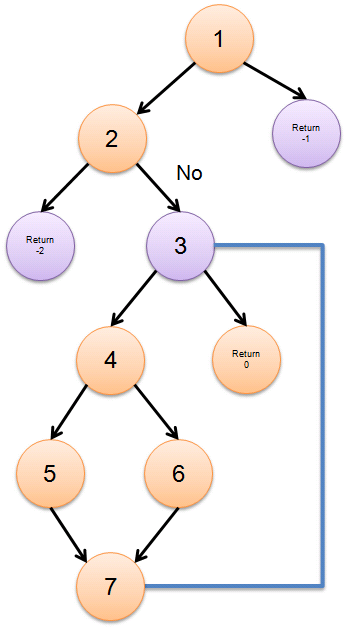
\includegraphics[width=0.45\textwidth]{./figures/flow.png}
\caption{Bitwalker\_Poke Flow}
\end{figure}

In this flow, 4 predicated nodes are displayed so, taking into account the equation V(g) = P + 1, where P are the predicate nodes, we see that the cyclomatic complexity of this function is V(g)=5.

\section{LocMetrics tool Results}

\href{http://www.locmetrics.com/}{[LocMetrics]} tool counts total lines of code (LOC), blank lines of code (BLOC), comment lines of code (CLOC), lines with both code and comments (C\&SLOC), logical source lines of code (SLOC-L), McCabe VG complexity (MVG), Header Comments (HCLOC), Header Words (HCWORD) and number of comment words (CWORDS). Physical executable source lines of code (SLOC-P) is calculated as the total lines of source code minus blank lines and comment lines. Counts are calculated on a per file basis and accumulated for the entire project. LocMetrics also generates a comment word histogram.

About the results obtained by LocMetrics tool are the following ones:

\begin{longtable}{||p{.125\textwidth}|p{.055\textwidth}|p{.065\textwidth}|p{.065\textwidth}|p{.055\textwidth}|p{.060\textwidth}|p{.09\textwidth}|p{.065\textwidth}|p{.085\textwidth}|p{.075\textwidth}|p{.1\textwidth}||}
  \caption{LocMetrics Tool Results}\\
    \hline\hline
    \textbf{File} & LOC &  SLOC-P & SLOC-L & MVG & BLOC & C\&SLOC & CLOC & CWORD & HCLOC & HCWORD \\
    \hline\hline
    \endhead
    \hline\hline
    \endfoot
    Bitwalker.h &
    42 & 15 & 12 & 0 & 8 & 1 & 19 & 102 & 0 & 0
    \\
    \hline
    Bitwalker.c &
    110 & 58 & 36 & 15 & 24 & 5 & 28 & 217 & 0 & 0
    \\
    \hline
    opnETCS.h &
    1250 & 884 & 883 & 0 & 181 & 637 & 185 & 3864 & 0 & 0
    \\
    \hline
    opnETCS
    \_Decoder.h &
    85 & 62 & 61 & 0 & 3 & 0 & 20 & 103 & 0 & 0
    \\
    \hline
\end{longtable}

\section{Understand tool Results}
\href{http://www.scitools.com/}{[Understand]} is a cross-platform, multi-language, maintenance-oriented IDE (Interactive Development Environment). It is designed to help maintain and understand large amounts of legacy or newly created source code. 
Understand also provides a way to check the code using coding Standard to avoid potencial errors. With this tool SQS has checked MISRA-C:2004 and code metrics (lines of code, complexity, object cross reference, invocation tree, Unused Items and others). The high recomended and mandatory techniques identified by CENELEC Standard covered by the tool are:
\begin{itemize}
\item Coding Standard (Mandatory)
\item Limited Size and Complexity in Functions, Subroutines and Methods (High Recomended)
\item Data Flow Analysis technique (High Recomended)
\item Control Flow Analysis technique (High Recomended)
\end{itemize}

The detailed static analysis report is available in the \href{https://github.com/openETCS/validation/tree/master/VnVUserStories/VnVUserStorySQS/04-Results}{[VnVUserStories folder]}

Below the \underline{MISRA-C tested rules} are listed:
\begin{itemize}
\item \textbf{Language extensions}
\begin{itemize}
\item 2.1 (req): Assembly language shall be encapsulated and isolated.
\item 2.2 (req): Source code shall only use \inl{/* ... */} style comments.
\item 2.3 (req): The character sequence \inl{/*} shall not be used within a comment.
\item 2.4 (adv-): Sections of code should not be 'commented out'.
\end{itemize}
\item \textbf{Character sets}
\begin{itemize}
\item 4.1 (req): Only those escape sequences that are defined in the ISO C standard shall be used.
\item 4.2 (req): Trigraphs shall not be used.
\end{itemize}
\item \textbf{Identifiers}
\begin{itemize}
\item 5.1 (req): Identifiers (internal and external) shall not rely on the significance of more than 31 characters.
\item 5.2 (req): Identifiers in an inner scope shall not use the same name as an identifier in an outer scope, and therefore hide that identifier.
\item 5.3 (req-): A \inl{typedef} name shall be a unique identifier.
\item 5.4 (req): A tag name shall be a unique identifier.
\item 5.5 (adv-): No object or function identifier with static storage duration should be reused.
\item 5.6 (adv-): No identifier in one name space should have the same spelling as an identifier in another name space, with the exception of structure and union member names.
\item 5.7 (adv-): No identifier name should be reused.
\end{itemize}
\item \textbf{Types}
\begin{itemize}
\item 6.3 (adv): \inl{typedef}s that indicate size and signedness should be used in place of the basic types.
\item 6.4 (req): Bit fields shall only be defined to be of type \inl{unsigned int} or \inl{signed int}.
\item 6.5 (req-): Bit fields of type signed int shall be at least 2 bits long.
\end{itemize}
\item \textbf{Constants}
\begin{itemize}
\item 7.1 (req): Octal constants (other than zero) and octal escape sequences shall not be used.
\end{itemize}
\item \textbf{Declarations and definitions}
\begin{itemize}
\item 8.5 (req-): There shall be no definitions of objects or functions in a header file.
\item 8.6 (adv): Functions shall be declared at file scope.
\item 8.7 (req): Objects shall be defined at block scope if they are only accessed from within a single function.
\item 8.8 (req): An external object or function shall be declared in one and only one file.
\item 8.9 (req): An identifier with external linkage shall have exactly one external definition.
\item 8.10 (req): All declarations and definitions of objects or functions at file scope shall have internal linkage unless external linkage is required.
\item 8.11 (req): The static storage class specifier shall be used in definitions and declarations of objects and functions that have internal linkage.
\end{itemize}
\item \textbf{Initialisation}
\begin{itemize}
\item 9.3 (req): In an enumerator list, the \inl{=} construct shall not be used to explicitly initialise members other than the first, unless all items are explicitly initialised.
\end{itemize}
\item \textbf{Control statement expressions}
\begin{itemize}
\item 13.3 (req): Floating-point expressions shall not be tested for equality or inequality.
\end{itemize}
\item \textbf{Control flow}
\begin{itemize}
\item 14.1 (req-): There shall be no unreachable code.
\item 14.3 (req-): Before preprocessing, a null statement shall only occur on a line by itself; it may be followed by a comment provided that the first character following the null statement is a white-space character.
\item 14.4 (req): The \inl{goto} statement shall not be used.
\item 14.5 (req): The \inl{continue} statement shall not be used.
\item 14.7 (req): A function shall have a single point of exit at the end of the function.
\item 14.10 (req): All \inl{if ... else if} constructs shall be terminated with an 'else' clause.
\end{itemize}
\item \textbf{Switch statements}
\begin{itemize}
\item 15.3 (req): The final clause of a \inl{switch} statement shall be the 
\inl{default} clause.
\end{itemize}
\item \textbf{Functions}
\begin{itemize}
\item 16.1 (req): Functions shall not be defined with variable numbers of arguments.
\item 16.2 (req): Functions shall not call themselves, either directly or indirectly.
\item 16.3 (req): Identifiers shall be given for all of the parameters in a function prototype declaration.
\item 16.4 (req-): The identifiers used in the declaration and definition of a function shall be identical.
\item 16.5 (req): Functions with no parameters shall be declared with parameter type void.
\end{itemize}
\item \textbf{Pointers and arrays}
\begin{itemize}
\item 17.5 (adv): The declaration of objects should contain no more than 2 levels of pointer indirection.
\end{itemize}
\item \textbf{Structures and unions}
\begin{itemize}
\item 18.4 (req): Unions shall not be used.
\end{itemize}
\item \textbf{Preprocessing directives}
\begin{itemize}
\item 19.1 (adv-): \inl{#include} statements in a file should only be preceded by other preprocessor directives or comments.
\item 19.2 (adv): Non-standard characters should not occur in header file names in include directives.
\item 19.3 (req): The \inl{#include} directive shall be followed by either a \inl{<filename>} or a \inl{<filename>} sequence.
\item 19.4 (req-): C macros shall only expand to a braced initializer, a constant, a parenthesised expression, a type qualifier, a storage class specifier, or a do-while-zero construct.
\item 19.5 (req): Macros shall not be \inl{#define}d or \inl{#undef}d within a block.
\item 19.6 (req): \inl{#undef} shall not be used.
\end{itemize}
\item \textbf{Standard libraries}
\begin{itemize}
\item 20.4 (req): Dynamic heap memory allocation shall not be used.
\item 20.5 (req): The error indicator \inl{errno} shall not be used.
\item 20.6 (req): The macro inl{offsetof}, in library \inl{<stddef.h>}, shall not be used.
\item 20.7 (req): The \inl{setjmp} macro and the \inl{longjmp} function shall not be used.
\item 20.8 (req): The signal handling facilities of \inl{<signal.h>} shall not be used.
\item 20.9 (req): The input/output library \inl{<stdio.h>} shall not be used in production code.
\item 20.10 (req): The library functions \inl{atof}, \inl{atoi} and \inl{atol} from library \inl{<stdlib.h>} shall not be used.
\item 20.11 (req): The library functions \inl{abort}, \inl{exit}, \inl{getenv} and \inl{system} from library \inl{<stdlib.h>} shall not be used.
\item 20.12 (req): The time handling functions of library \inl{<time.h>} shall not be used.
\end{itemize}
\item \textbf{Run-time failures}
\begin{itemize}
\item 21.1 (req-): Minimization of run-time failures shall be ensured by the use of at least one of: 
\begin{itemize}
\item static analysis tools/techniques;
\item dynamic analysis tools/techniques;
\item explicit coding of checks to handle run-time faults.
\end{itemize}
\end{itemize}
\end{itemize}
 
After a review of the subset of MISRA-C rules taking into account project requirements and sector standard or best practices it is necessary to decide which of some of them are not to be implemented/approved due to its application can get worse understanbility of the code and which other rules of other standard will be applied.

The table below shows the non approved MISRA-C rules.

{\footnotesize\sffamily\centering
  \begin{longtable}{||p{.15\textwidth}|p{.15\textwidth}||}
  \caption{Status of MISRA Rules}\\
    \hline\hline
    \textbf{MISRA Rule} & \textbf{Status} \\
    \hline\hline
    \endhead
    \hline\hline
    \endfoot
    \textbf{Global 5.1}
& no recommended
    \\
    \hline
    \textbf{Global 5.6}
& no recommended
    \\
    \hline
\end{longtable}}


The results of the MISRA Rules are the following:
\begin{figure}[H]
\centering
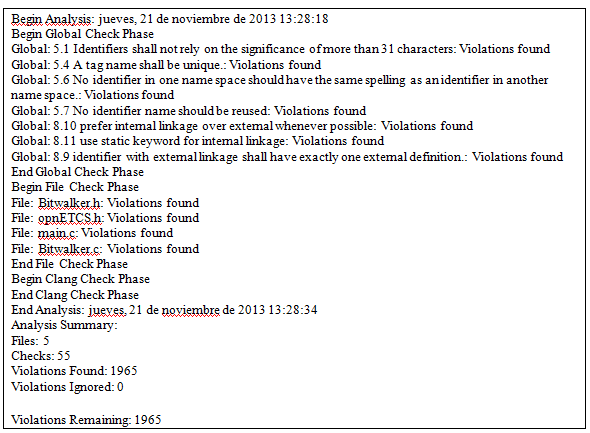
\includegraphics{./figures/understand.png}
\caption{MISRA-C Rules results}
\end{figure}

The files into the violations are found are listed in the below table.

{\footnotesize\sffamily\centering
  \begin{longtable}{||p{.15\textwidth}|p{.8\textwidth}||}
  \caption{Summary of detected MISRA Violations}\\
    \hline\hline
    \textbf{MISRA Rule} & \textbf{Files} \\
    \hline\hline
    \endhead
    \hline\hline
    \endfoot
    \textbf{Global 5.1}
& Bitwalker.c/opnETCS.h/opnETCS\_Decoder.h
    \\
    \hline
    \textbf{Global 5.4}
& opnETCS.h
    \\
    \hline
    \textbf{Global 5.6}
& Bitwalker.c/Bitwalker.h
    \\
    \hline
    \textbf{Global 5.7}
& Bitwalker.c/Bitwalker.h/opnETCS.h
    \\
    \hline
    \textbf{Global 8.9}
& opnETCS\_Decoder.h
    \\
    \hline
    \textbf{Global 8.10}
& main.c
    \\
    \hline
    \textbf{Global 8.11}
& main.c
    \\
    \hline
\end{longtable}}

A detailed information about the file, entity, line, check, etc of all violations detected above can be found in the index files of \href{https://github.com/openETCS/validation/blob/master/VnVUserStories/VnVUserStorySQS/04-Results/results}{[Results]} and \href{https://github.com/openETCS/validation/blob/master/VnVUserStories/VnVUserStorySQS/04-Results/results2}{[Results2]} folders.

In addition to the MISRA-C compliance checking, we also run code metrics analysis in order to ensure the correctness of the obtained results through the results comparation.

Below tables shows some different metrics per file and function.
In order to understand the tables and to be able to compare the results obtained with the different tools the definition of the specific metrics is provided before the presentation of the corresponding table.
\begin{itemize}
\item Cyclomatic: The measure of the complexity of a function's decision structure. The cyclomatic complexity is also the number of basis, or independent, paths through a module. 
\item Modified Cyclomatic: cyclomatic except each case statement is not counted;the entire switch counts as 1.
\item Strict: Cyclomatic complexity except each short-circuit operator adds 1 to the complexity.
\item Essential Complexity: cyclomatic complexity after structured programming constructs have been removed.
\item Nesting: maximum nesting level of control constucts (if, while,etc.)
\item Count Path: Number of unique paths through a body of code (not counting gotos or abnormal exits
\end{itemize}


\begin{longtable}{||p{.275\textwidth}|p{.0025\textwidth}||}
  \caption{Function Complexity metrics}\\
    \hline\hline
    \endhead
    \hline\hline
    \endfoot
\multicolumn{2}{||l||}{\textbf{Bitwalker\_Peek}}
\\\hline
\ Cyclomatic: & 3
\\\hline
\ Modified Cyclomatic: & 3
\\\hline
\ Strict Cyclomatic: & 3
\\\hline
\ Essential: & 1
 \\\hline
\ Max Nesting:   & 1
 \\\hline
\ Count Path: & 3
\\\hline
\multicolumn{2}{||l||}{\textbf{Bitwalker\_Poke}}
\\\hline
\ Cyclomatic: & 5
\\\hline
\ Modified Cyclomatic: & 5
\\\hline
\ Strict Cyclomatic: & 5
\\\hline
\ Essential: & 3
 \\\hline
\ Max Nesting:   & 2
 \\\hline
\ Count Path: & 5
\\\hline
\multicolumn{2}{||l||}{\textbf{Bitwalker\_IncrementalWalker\_Init}}
\\\hline
\ Cyclomatic: & 1
\\\hline
\ Modified Cyclomatic: & 1
\\\hline
\ Strict Cyclomatic: & 1 
\\\hline
\ Essential: & 1
 \\\hline
\ Max Nesting:   & 0
 \\\hline
\ Count Path: & 1
\\\hline
\multicolumn{2}{||l||}{\textbf{Bitwalker\_IncrementalWalker\_Peek\_Next}}
\\\hline
\ Cyclomatic: & 1
\\\hline
\ Modified Cyclomatic: & 1
\\\hline
\ Strict Cyclomatic: & 1 
\\\hline
\ Essential: & 1
 \\\hline
\ Max Nesting:   & 0
 \\\hline
\ Count Path: & 1
\\\hline
\multicolumn{2}{||l||}{\textbf{Bitwalker\_IncrementalWalker\_Peek\_Finish}}
\\\hline
\ Cyclomatic: & 1
\\\hline
\ Modified Cyclomatic: & 1
\\\hline
\ Strict Cyclomatic: & 1 
\\\hline
\ Essential: & 1
 \\\hline
\ Max Nesting:   & 0
 \\\hline
\ Count Path: & 1
\\\hline
\multicolumn{2}{||l||}{\textbf{Bitwalker\_IncrementalWalker\_Poke\_Next}}
\\\hline
\ Cyclomatic: & 1
\\\hline
\ Modified Cyclomatic: & 1
\\\hline
\ Strict Cyclomatic: & 1 
\\\hline
\ Essential: & 1
 \\\hline
\ Max Nesting:   & 0
 \\\hline
\ Count Path: & 1
\\\hline
\multicolumn{2}{||l||}{\textbf{Bitwalker\_IncrementalWalker\_Poke\_Finish}}
\\\hline
\ Cyclomatic: & 1
\\\hline
\ Modified Cyclomatic: & 1
\\\hline
\ Strict Cyclomatic: & 1 
\\\hline
\ Essential: & 1
 \\\hline
\ Max Nesting:   & 0
 \\\hline
\ Count Path: & 1
\\\hline
\end{longtable}

Here are some remarks about how the Understand tool defines and take into account the following code metrics:
\begin{itemize}
\item Lines: total lines (in a function or file or project)
\item Comment Lines: total lines that have comments on them
\item Blank Lines: total lines without any code/comment
\item Code Lines: total lines that have any code on them
\item Executable Lines: total lines that have executable code on them
\item Declarative Lines: total lines that have declarative code on them
\item Execution Statements: total statements in executable code
\item Declaration Statements: total statements in declarative code
\item Ratio Comment/Code: comment lines / code lines
\end{itemize}

\begin{longtable}{||p{.275\textwidth}|p{.125\textwidth}|p{.125\textwidth}|p{.125\textwidth}|p{.125\textwidth}|p{.125\textwidth}||}
  \caption{File Metrics}\\
    \hline\hline
    \textbf{Metrics} & \textbf{Bitwalker.h} & \textbf{Bitwalker.c} & \textbf{opnETCS.h} & \textbf{opnETCS \_Decoder.h}\\
    \hline\hline
    \endhead
    \hline\hline
    \endfoot
    \ Lines: & 41
& 109
& 1249 & 84
    \\
    \hline
    \ Comment Lines: & 20
& 33
& 822 & 20
    \\
    \hline
    \ Blank Lines: & 7
& 23
& 180 & 2
    \\
    \hline
    \ Preprocessor Lines: & 4
& 1
& 1 & 1
    \\
    \hline
    \ Code Lines:  & 11
& 57
& 883 & 61
    \\
    \hline
    \ Inactive Lines:  & 0
& 0
& 0 & 0
    \\
    \hline
    \ Executable Code Lines:  & 0
& 30
& 0 & 0
    \\
    \hline
    \ Declarative Code Lines:  & 11
& 15
& 822 & 61
    \\
    \hline
    \ Execution Statements:  & 0
& 28
& 0 & 0
    \\
    \hline
    \ Declaration Statements:  & 11
& 15
& 760 & 61
    \\
    \hline
    \ Ratio Comment/Code:  & 1.82
& 0.58
& 0.93 & 0.33
    \\
    \hline
    \ Units  & 0
& 7
& 0 & 0
    \\
    \hline
   \end{longtable}
   

\begin{longtable}{||p{.350\textwidth}|p{.0125\textwidth}||}
  \caption{Function code Metrics}\\
    \hline\hline
    \endhead
    \hline\hline
    \endfoot
    \multicolumn{2}{||l||}{\textbf{Bitwalker\_IncrementalWalker\_Init}}
\\\hline
    \ Lines: & 6
    \\
    \hline
    \ Comment Lines: & 0
    \\
    \hline
    \ Blank Lines: & 0
    \\
    \hline
    \ Code Lines:  & 6
    \\
    \hline
    \ Inactive Lines:  & 0
    \\
    \hline
    \ Executable Code Lines:  & 3
    \\
    \hline
    \ Declarative Code Lines:  & 1
    \\
    \hline
    \ Execution Statements:  & 3
    \\
    \hline
    \ Declaration Statements:  & 0
    \\
    \hline
    \ Ratio Comment/Code:  & 0.00
    \\
    \hline
    \multicolumn{2}{||l||}{\textbf{Bitwalker\_IncrementalWalker\_Peek\_Finish}}
\\\hline
    \ Lines: & 4
    \\
    \hline
    \ Comment Lines: & 0
    \\
    \hline
    \ Blank Lines: & 0
    \\
    \hline
    \ Code Lines:  & 4
    \\
    \hline
    \ Inactive Lines:  & 0
    \\
    \hline
    \ Executable Code Lines:  & 1
    \\
    \hline
    \ Declarative Code Lines:  & 1
    \\
    \hline
    \ Execution Statements:  & 1
    \\
    \hline
    \ Declaration Statements:  & 0
    \\
    \hline
    \ Ratio Comment/Code:  & 0.00
    \\
    \hline
    \multicolumn{2}{||l||}{\textbf{Bitwalker\_IncrementalWalker\_Peek\_Next}}
\\\hline
    \ Lines: & 7
    \\
    \hline
    \ Comment Lines: & 1
    \\
    \hline
    \ Blank Lines: & 0
    \\
    \hline
    \ Code Lines:  & 6
    \\
    \hline
    \ Inactive Lines:  & 0
    \\
    \hline
    \ Executable Code Lines:  & 3
    \\
    \hline
    \ Declarative Code Lines:  & 2
    \\
    \hline
    \ Execution Statements:  & 2
    \\
    \hline
    \ Declaration Statements:  & 1
    \\
    \hline
    \ Ratio Comment/Code:  & 0.17
    \\
    \hline
    \multicolumn{2}{||l||}{\textbf{Bitwalker\_IncrementalWalker\_Poke\_Finish}}
\\\hline
    \ Lines: & 4
    \\
    \hline
    \ Comment Lines: & 0
    \\
    \hline
    \ Blank Lines: & 0
    \\
    \hline
    \ Code Lines:  & 4
    \\
    \hline
    \ Inactive Lines:  & 0
    \\
    \hline
    \ Executable Code Lines:  & 1
    \\
    \hline
    \ Declarative Code Lines:  & 1
    \\
    \hline
    \ Execution Statements:  & 1
    \\
    \hline
    \ Declaration Statements:  & 0
    \\
    \hline
    \ Ratio Comment/Code:  & 0.00
    \\
    \hline
    \multicolumn{2}{||l||}{\textbf{Bitwalker\_IncrementalWalker\_Poke\_Next}}
\\\hline
    \ Lines: & 7
    \\
    \hline
    \ Comment Lines: & 1
    \\
    \hline
    \ Blank Lines: & 0
    \\
    \hline
    \ Code Lines:  & 6
    \\
    \hline
    \ Inactive Lines:  & 0
    \\
    \hline
    \ Executable Code Lines:  & 3
    \\
    \hline
    \ Declarative Code Lines:  & 2
    \\
    \hline
    \ Execution Statements:  & 2
    \\
    \hline
    \ Declaration Statements:  & 1
    \\
    \hline
    \ Ratio Comment/Code:  & 0.17
    \\
    \hline
    \multicolumn{2}{||l||}{\textbf{Bitwalker\_Peek}}
\\\hline
    \ Lines: & 20
    \\
    \hline
    \ Comment Lines: & 5
    \\
    \hline
    \ Blank Lines: & 4
    \\
    \hline
    \ Code Lines:  & 13
    \\
    \hline
    \ Inactive Lines:  & 0
    \\
    \hline
    \ Executable Code Lines:  & 7
    \\
    \hline
    \ Declarative Code Lines:  & 4
    \\
    \hline
    \ Execution Statements:  & 7
    \\
    \hline
    \ Declaration Statements:  & 3
    \\
    \hline
    \ Ratio Comment/Code:  & 0.38
    \\
    \hline
        \multicolumn{2}{||l||}{\textbf{Bitwalker\_Poke}}
\\\hline
    \ Lines: & 24
    \\
    \hline
    \ Comment Lines: & 6
    \\
    \hline
    \ Blank Lines: & 4
    \\
    \hline
    \ Code Lines:  & 17
    \\
    \hline
    \ Inactive Lines:  & 0
    \\
    \hline
    \ Executable Code Lines:  & 11
    \\
    \hline
    \ Declarative Code Lines:  & 3
    \\
    \hline
    \ Execution Statements:  & 12
    \\
    \hline
    \ Declaration Statements:  & 2
    \\
    \hline
    \ Ratio Comment/Code:  & 0.35
    \\
    \hline
   \end{longtable}

Taking into account control flow and data flow techniques some Uninitialized Items (items such as variables that are not initialized in the code), Unused Variables and Parameters items (items that are declared (and perhaps initialized) but never referenced other than that) and Unused Program Units have been identified. The Unused Program Units Report identifies program units that are declared but never used. However note that this listing in this report doesnt mean the system doesnt need this program unit.

{\footnotesize\sffamily\centering
  \begin{longtable}{||p{.15\textwidth}|p{.40\textwidth}|p{.15\textwidth}|p{.15\textwidth}||}
  \caption{Unused Variables and Parameters}\\
    \hline\hline
    \textbf{File} & \textbf{Item} & \textbf{Type of Item} & \textbf{Location} \\
    \hline\hline
    \endhead
    \hline\hline
    \endfoot
    \textbf{Bitwalker.c}
& Bitwalker\_IncrementalWalker\_Peek\_Finish & Function & line 91
    \\
    \hline
    \textbf{Bitwalker.c}
& Bitwalker\_IncrementalWalker\_Peek\_Next & Function & line 82
    \\
    \hline
    \textbf{Bitwalker.c}
& Bitwalker\_IncrementalWalker\_Poke\_Finish & Function & line 106
    \\
    \hline
\end{longtable}}

{\footnotesize\sffamily\centering
  \begin{longtable}{||p{.15\textwidth}|p{.15\textwidth}|p{.15\textwidth}||}
  \caption{Uninitialized Items}\\
    \hline\hline
    \textbf{File} & \textbf{Item} & \textbf{Location} \\
    \hline\hline
    \endhead
    \hline\hline
    \endfoot
    \textbf{Bitwalker.c}
& i & line 35
    \\
    \hline
    \textbf{Bitwalker.c}
& i & line 60
    \\
    \hline
\end{longtable}}

{\footnotesize\sffamily\centering
  \begin{longtable}{||p{.15\textwidth}|p{.40\textwidth}|p{.15\textwidth}||}
  \caption{Unused Program Units}\\
    \hline\hline
    \textbf{File} & \textbf{Item} & \textbf{Location} \\
    \hline\hline
    \endhead
    \hline\hline
    \endfoot
    \textbf{Bitwalker.c}
& Bitwalker\_IncrementalWalker\_Peek\_Finish & line 91
    \\
    \hline
    \textbf{Bitwalker.c}
& Bitwalker\_IncrementalWalker\_Peek\_Next & line 82
    \\
    \hline
    \textbf{Bitwalker.c}
& Bitwalker\_IncrementalWalker\_Poke\_Finish & line 106
    \\
    \hline
\end{longtable}}

\section{Clang Static Analyzer tool Results}
The \href{http://clang-analyzer.llvm.org/}{[Clang Static Analyzer]} is a source code analysis tool that finds bugs in C, C++, and Objective-C programs.

The analyzer is 100\% open source and is part of the Clang project. Like the rest of Clang, the analyzer is implemented as a C++ library that can be used by other tools and applications.

With this analysis SQS has checked the following:

{\footnotesize\sffamily\centering
  \begin{longtable}{||p{.45\textwidth}|p{.5\textwidth}||}
  \caption{Aspects checked}\\
    \hline\hline
    \hline\hline
    \endhead
    \hline\hline
    \endfoot
    \textbf{core.AdjustedReturnValue}
& Check to see if the return value of a function call is different than the caller expects (e.g., from calls through function pointers).
    \\
    \hline
    \textbf{core.CallAndMessage}
& Check for logical errors for function calls and Objective-C message expressions (e.g., uninitialized arguments, null function pointers).
    \\
    \hline
    \textbf{core.DivideZero}
& Check for division by zero.
    \\
    \hline
    \textbf{core.NonNullParamChecker}
& Check for null pointers passed as arguments to a function whose arguments are known to be non-null.
    \\
    \hline
    \textbf{core.NullDereference}
& Check for dereferences of null pointers.
    \\
    \hline
    \textbf{core.StackAddressEscape}
& Check that addresses to stack memory do not escape the function.
    \\
    \hline
    \textbf{core.UndefinedBinaryOperatorResult}
& Check for undefined results of binary operators.
    \\
    \hline
    \textbf{core.VLASize}
& Check for declarations of VLA of undefined or zero size.
    \\
    \hline
    \textbf{core.builtin.BuiltinFunctions}
& Evaluate compiler built-in functions (e.g., alloca()).
    \\
    \hline
    \textbf{core.builtin.NoReturnFunctions}
& Evaluate "panic" functions that are known to not return to the caller.
    \\
    \hline
    \textbf{core.uninitialized.ArraySubscript}
& Check for uninitialized values used as array subscripts.
    \\
    \hline
    \textbf{core.uninitialized.Assign}
& Check for assigning uninitialized values.
    \\
    \hline
    \textbf{core.uninitialized.Branch}
& Check for uninitialized values used as branch conditions.
    \\
    \hline
    \textbf{core.uninitialized.CapturedBlockVariable}
& Check for blocks that capture uninitialized values.
    \\
    \hline
    \textbf{core.uninitialized.UndefReturn}
& Check for uninitialized values being returned to the caller.
    \\
    \hline
    \textbf{deadcode.DeadStores}
& Check for values stored to variables that are never read afterwards.
    \\
    \hline
    \textbf{security.FloatLoopCounter}
& Warn on using a floating point value as a loop counter (CERT: FLP30-C, FLP30-CPP).
    \\
    \hline
    \textbf{security.insecureAPI.UncheckedReturn}
& Warn on uses of functions whose return values must be always checked.
    \\
    \hline
    \textbf{security.insecureAPI.getpw}
& Warn on uses of the 'getpw' function.
    \\
    \hline
    \textbf{security.insecureAPI.gets}
& Warn on uses of the 'gets' function.
    \\
    \hline
    \textbf{security.insecureAPI.mkstemp}
& Warn when 'mkstemp' is passed fewer than 6 X's in the format string.
    \\
    \hline
    \textbf{security.insecureAPI.mktemp}
& Warn on uses of the 'mktemp' function.
    \\
    \hline
    \textbf{security.insecureAPI.rand}
& Warn on uses of the 'rand', 'random', and related functions.
    \\
    \hline
    \textbf{security.insecureAPI.strcpy}
& Warn on uses of the 'strcpy' and 'strcat' functions.
    \\
    \hline
    \textbf{security.insecureAPI.vfork}
& Warn on uses of the 'vfork' function.
    \\
    \hline
    \textbf{unix.API}
& Check calls to various UNIX/Posix functions.
    \\
    \hline
    \textbf{unix.Malloc}
& Check for memory leaks, double free, and use-after-free problems involving malloc.
    \\
    \hline
    \textbf{unix.MallocSizeof}
& Check for dubious malloc arguments involving sizeof.
    \\
    \hline
    \textbf{unix.MismatchedDeallocator}
& Check for mismatched deallocators (e.g. passing a pointer allocating with new to free()).
    \\
    \hline
    \textbf{unix.cstring.BadSizeArg}
& Check the size argument passed into C string functions for common erroneous patterns.
    \\
    \hline
    \textbf{unix.cstring.NullArg}
& Check for null pointers being passed as arguments to C string functions.
    \\
    \hline
\end{longtable}}

Taking into account the features checked by the tool, the following Cenelec Standard techniques have been covered:
\begin{itemize}
\item Boundary Value Analysis (High Recommended)
\item Data Flow Analysis (High Recommended)
\end{itemize}

After run this analysis no violation has been found.

\begin{figure}[H]
\centering
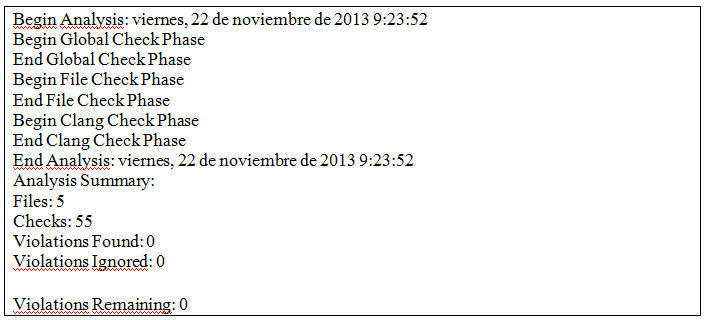
\includegraphics[scale=0.8]{./figures/clang.png}
\caption{Clang Analysis results}
\end{figure}

\section{CPPcheck tool Results}

Bitwalker folder has been analyzed statically by \href{http://cppcheck.sourceforge.net/}{[CPPcheck]} tool (Complying with the standard C11).

Cppcheck supports the following languages: C89, C99, C11 and a wide variety of static checks. The following features are provided:
\begin{itemize}
\item Out of bounds checking
\item Check the code for each class
\item Checking exception safety
\item Memory leaks checking
\item Warn if obsolete functions are used
\item Check for invalid usage of STL
\item Check for uninitialized variables and unused functions
\item Check input/output operations
\item Null pointer dereferencing
\end{itemize}

C11 (formerly C1X) is an informal name for ISO/IEC 9899:2011, the current standard for the C programming language. It replaces the previous C standard, informally known as C99. This new version mainly standardizes features that have already been supported by common contemporary compilers, and includes a detailed memory model to better support multiple threads of execution. Due to delayed availability of conforming C99 implementations, C11 makes certain features optional, to make it easier to comply with the core language standard.

With the use of this tool the following techniques recommended by CENELEC Standard are covered:
\begin{itemize}
\item Coding Standard (mandatory) (checked C11 standard)
\item Boundary Value Analysis (High Recommended)
\item Data Flow Analysis (High Recommended)
\end{itemize}

The results of the tool show that there are some verbose errors in the main file and some errors in the bitwalker.c file.

\begin{itemize}
\item repetitive verbose error regarding to Testwort variable is reassigned value before the old one has been used (lines 119, 120 and 121 in main.c)
\item one error about the Testwort variable is assigned a value that is never used (line 122 in main.c).
\item the funtions Bitwalker\_IncrementalWalker\_Peek\_Finish (line 91 in bitwalker.c), Bitwalker\_IncrementalWalker\_Peek\_Next (line 82 in bitwalker.c) and Bitwalker\_IncrementalWalker\_Poke\_Finish (line 106 in bitwalker.c) are never used,
\end{itemize}  

The below figure shows the results commented previously:
\begin{figure}[H]
\centering
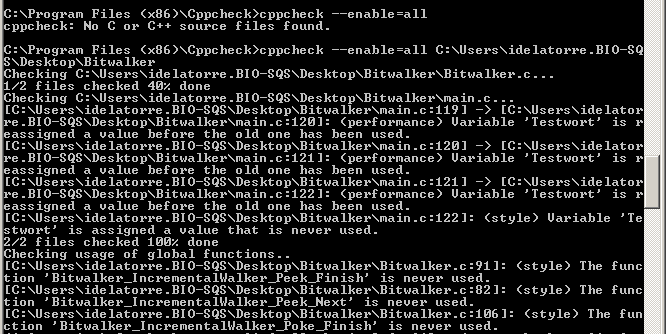
\includegraphics{./figures/cppcheck.png}
\caption{cppcheck results}
\end{figure}

\section{Testwell CMT++ Results}
\label{sec:halsted}
CMT++, Complexity Measures Tool for C/C++, is an easy-to-use code metrics tool for C and C++ languages. Also assembly code, either inlined in a C/C++ source file or separate assembly file, can be measured.

Based on the static properties of the program code CMT++ gives estimates how error prone the program sorce code is due to its complexity, how long it will take to understand the code, what the logical volume of the code is, how much code you have: physical lines, comment lines, program lines, statements, etc

CMT++ helps to estimate the overall maintainability of the code base and easily locate the complex parts of it. 

In this case CMT++ is used to calculate:
\begin{itemize}
\item Basic code complexity metrics
\begin{itemize}
\item McCabe's cyclomatic number
\item Halstead's metrics
\item Lines of code metrics
\item Some other metrics like: number of semicolons, number of function parameter, depth of control structure nesting
\end{itemize}
\item Maintainability Index
\end{itemize}

\subsection{Complexity Metrics}
\subsubsection{Program Size Metrics}
As it was mentioned in \ref{sec:sizem} the number of lines and the Halsted metrics can be used to determine the program size.
\begin{description}
\item \textbf{Number of lines}

The lines of code measures are the most traditional measures used to quantify software complexity. They are simple, easy to count, and very easy to understand. However, they do not take into account the intelligence content and the layout of the code.

CMT++ calculates the following lines-of-code metrics:
\begin{itemize}
\item LOCphy: number of physical lines
\item LOCbl: number of blank lines (a blank line inside a comment block is considered to be a comment line)
\item LOCpro: number of program lines (declarations, definitions, directives, and code)
\item LOCcom: number of comment lines
\end{itemize}

Following the analysis conducted within the tool, the tables below summarizes the results:

\begin{longtable}{||p{.475\textwidth}|p{.115\textwidth}|p{.115\textwidth}|p{.115\textwidth}|p{.115\textwidth}||}
  \caption{Lines of Code Metrics per file}\\
    \hline\hline
    \textbf{File} &\textbf{LOCphy} & \textbf{LOCpro} & \textbf{LOCcom} & \textbf{LOCbl}\\
    \hline\hline
    \endhead
    \hline\hline
    \endfoot
    Bitwalker.c & 109 & 58 & 33 & 23
    \\
    \hline
   \end{longtable}
   
\begin{longtable}{||p{.475\textwidth}|p{.115\textwidth}|p{.115\textwidth}|p{.115\textwidth}|p{.115\textwidth}||}
  \caption{Lines of Code Metrics per functions}\\
    \hline\hline
    \textbf{Function} &\textbf{LOCphy} & \textbf{LOCpro} & \textbf{LOCcom} & \textbf{LOCbl}\\
    \hline\hline
    \endhead
    \hline\hline
    \endfoot
    Bitwalker\_Peek & 20 & 13 & 5 & 4
    \\
    \hline
    Bitwalker\_Poke & 24 & 17 & 6 & 4
    \\
    \hline
    Bitwalker\_IncrementalWalker\_Init & 6 & 6 & 0 & 0
    \\
    \hline
    Bitwalker\_IncrementalWalker\_Peek\_Next & 7 & 6 & 1 & 0
    \\
    \hline
    Bitwalker\_IncrementalWalker\_Peek\_Finish & 4 & 4 & 0 & 0
    \\
    \hline
    Bitwalker\_IncrementalWalker\_Poke\_Next & 7 & 6 & 1 & 0
    \\
    \hline
    Bitwalker\_IncrementalWalker\_Poke\_Finish & 4 & 4 & 0 & 0
    \\
    \hline
   \end{longtable}

\item \textbf{Halsted metrics}

Halstead complexity metrics were developed by the late Maurice Halstead as a means of determining a quantitative measure of complexity directly from the operators and operands in the module to measure a program module's complexity directly from source code.

Halstead's metrics are based on interpreting the source code as a sequence of tokens and classifying each token to be an operator or an operand. There are based on four basic measures:
\begin{itemize}
\item number of unique (distinct) operators ($n_1$)
\item number of unique (distinct) operands ($n_2$)
\item total number of operators ($N_1$)
\item total number of operands ($N_2$).
\end{itemize}

Taking into account these measures the following metrics will be obtained:
\begin{itemize}
\item Program Vocabulary: $n = n_1 + n_2$
\item Program Length: $N = N_1 + N_2$
\item Program Difficulty: $D = ( n_1 / 2 ) * ( N_2 / n_2 )$
\item Program Volume: $V = N * log_2 (n)$
\item Program Length: L = 1/V
\item Effort to implement: E = V * D
\item Time to implement: T = E / 18
\item Number of delivered bugs: $B = (E^{2/3}) / 3000$
\end{itemize}

So Halsted metrics provide several metrics that focus on different aspects of software complexity. Furthermore, they allow the estimation of development and testing times (with parameter L*V), and difficulty of understanding (with parameter E). 

Software complexity is usually analyzed with the indicators L, V and E due to:
\begin{itemize}
\item the volume is intended being a more accurate measure of the difficulty of understanding a program, taking into account not only its length but also the vocabulary. Halstead's volume (V) describes the size of the implementation of an algorithm.
\item the program level gives an idea of ​​the level of detail that it has been encoded
\item effort can be used as a measure of program clarity since the effort required to produce a piece of software is primarily related to the difficulty to understand and implement it.
\end{itemize}

In the tables below are presented the results obtained per file and per functions:

\begin{longtable}{||p{.475\textwidth}|p{.070\textwidth}|p{.060\textwidth}|p{.060\textwidth}|p{.060\textwidth}|p{.060\textwidth}|p{.060\textwidth}|p{.060\textwidth}||}
  \caption{Halsted metrics 1 per file}\\
    \hline\hline
    \textbf{File} &\textbf{L} & \textbf{n} & \textbf{$n_1$} & \textbf{$n_2$} & \textbf{N} & \textbf{$N_1$} & \textbf{$N_2$}\\
    \hline\hline
    \endhead
    \hline\hline
    \endfoot
    Bitwalker.c & 0.014 & 72 & 31 & 41 & 378 & 185 & 193
    \\
    \hline
   \end{longtable}
   
\begin{longtable}{||p{.475\textwidth}|p{.070\textwidth}|p{.125\textwidth}|p{.085\textwidth}|p{.075\textwidth}|p{.090\textwidth}||}
  \caption{Halsted metrics 2 per file}\\
    \hline\hline
    \textbf{File} &\textbf{B} & \textbf{E} & \textbf{T} & \textbf{D} & \textbf{V}\\
    \hline\hline
    \endhead
    \hline\hline
    \endfoot
    Bitwalker.c & 1.024 & 170167.578 & 02:37:33 & 72.963 & 2332.232 
    \\
    \hline
   \end{longtable}
   
\begin{longtable}{||p{.475\textwidth}|p{.070\textwidth}|p{.060\textwidth}|p{.060\textwidth}|p{.060\textwidth}|p{.060\textwidth}|p{.060\textwidth}|p{.060\textwidth}||}
  \caption{Halsted metrics 1 per functions}\\
    \hline\hline
    \textbf{Function} &\textbf{L} & \textbf{n} & \textbf{$n_1$} & \textbf{$n_2$} & \textbf{N} & \textbf{$N_1$} & \textbf{$N_2$}\\
    \hline\hline
    \endhead
    \hline\hline
    \endfoot
    Bitwalker\_Peek & 0.041 & 35 & 18 & 17 & 89 & 43 & 46
    \\
    \hline
    Bitwalker\_Poke & 0.028 & 42 & 23 & 19 & 120 & 62 & 58
    \\
    \hline
    Bitwalker\_IncrementalWalker\_Init & 0.143 & 20 & 8 & 12 & 37 & 16 & 21
    \\
    \hline
    Bitwalker\_IncrementalWalker\_Peek\_Next & 0.116 & 20 & 9 & 11 & 39 & 18 & 21
    \\
    \hline
    Bitwalker\_IncrementalWalker\_Peek\_Finish & 0.278 & 11 & 6 & 5 & 12 & 6 & 6
    \\
    \hline
    Bitwalker\_IncrementalWalker\_Poke\_Next & 0.111 & 21 & 9 & 12 & 44 & 20 & 24
    \\
    \hline
    Bitwalker\_IncrementalWalker\_Poke\_Finish & 0.278 & 11 & 6 & 5 & 12 & 6 & 6
    \\
    \hline
   \end{longtable}
   
\begin{longtable}{||p{.475\textwidth}|p{.070\textwidth}|p{.1\textwidth}|p{.085\textwidth}|p{.075\textwidth}|p{.080\textwidth}||}
  \caption{Halsted metrics 2 per functions}\\
    \hline\hline
    \textbf{Function} &\textbf{B} & \textbf{E} & \textbf{T} & \textbf{D} & \textbf{V}\\
    \hline\hline
    \endhead
    \hline\hline
    \endfoot
    Bitwalker\_Peek & 0.166 & 11117.269 & 00:10:17 & 24.353 & 456.506 
    \\
    \hline
    Bitwalker\_Poke & 0.267 & 22715.846 & 00:21:01 & 35.105 & 647.078 
    \\
    \hline
    Bitwalker\_IncrementalWalker\_Init & 0.036 & 1119.379 & 00:01:02 & 7.000 & 159.911 
    \\
    \hline
    Bitwalker\_IncrementalWalker\_Peek\_Next & 0.043 & 1448.042 & 00:01:20 & 8.591 & 168.555 
    \\
    \hline
    Bitwalker\_IncrementalWalker\_Peek\_Finish & 0.009 & 149.447 & 00:00:08 & 3.600 & 41.513 
    \\
    \hline
    Bitwalker\_IncrementalWalker\_Poke\_Next & 0.048 & 1739.358 & 00:01:36 & 9.000 & 193.262 
    \\
    \hline
    Bitwalker\_IncrementalWalker\_Poke\_Finish & 0.009 & 149.447 & 00:00:08 & 3.600 & 41.513 
    \\
    \hline
   \end{longtable}

\end{description}

The volume of a function should be at least 20 and at most 1000. The volume of a parameter less one-line function that is not empty; is about 20. A volume greater than 1000 tells that the function probably does too many things.

The volume of a file should be at least 100 and at most 8000. These limits are based on volumes measured for files whose LOCpro and v(G) are near their recommended limits. The limits of volume can be used for double-checking.

Halstead's delivered bugs (B) is an estimate for the number of errors in the implementation.
Delivered bugs in a file should be less than 2. 
Experiences have shown that, when programming with C or C++, a source file almost always contains more errors than B suggests. The number of defects tends to grow more rapidly than B.

By analyzing the results, one can observe that all the Halsted metrics obtained in relation to functions and file are inside the recommendations.


\subsubsection{Control Flow Metrics}
\begin{longtable}{||p{.475\textwidth}|p{.075\textwidth}||}
  \caption{McCabe Cyclomatic Complexity}\\
    \hline\hline
    \textbf{Function} &\textbf{ECC}\\
    \hline\hline
    \endhead
    \hline\hline
    \endfoot
    Bitwalker\_Peek & 3  
    \\
    \hline
    Bitwalker\_Poke & 5  
    \\
    \hline
    Bitwalker\_IncrementalWalker\_Init & 1
    \\
    \hline
    Bitwalker\_IncrementalWalker\_Peek\_Next & 1  
    \\
    \hline
    Bitwalker\_IncrementalWalker\_Peek\_Finish & 1  
    \\
    \hline
    Bitwalker\_IncrementalWalker\_Poke\_Next & 1  
    \\
    \hline
    Bitwalker\_IncrementalWalker\_Poke\_Finish & 1  
    \\
    \hline
   \end{longtable}

As a first conclusion, taking into account the reference table shown in Section \ref{sec:cyclo} the values from the above table indicate a low risk functions and the matching with the results obtained with the previous tools.

\subsection{Maintainability Index}
Maintainability Index (MI) is a single-number value for estimating the relative maintainability of the code.

Maintainability Index is calculated with certain formulae from lines-of-code measures, McCabe measure and Halstead measures.

Actually there are three measures:
\begin{itemize}
\item MIwoc: Maintainability Index without comments
\item MIcw: Maintainability Index comment weight
\item MI: Maintainability Index = MIwoc + MIcw
\end{itemize}

The general formulae for MI is the following:

MIwoc = 171 - 5.2 * ln(aveV) -0.23 * aveG -16.2 * ln(aveLOC)

MIcw = 50 * sin(sqrt(2.4 * perCM))

MI = MIwoc + MIcw

where:
\begin{itemize}
\item aveV = average Halstead Volume per Module
\item aveG = average extended cyclomatic complexity per Module
\item aveLOC = average count of lines per Module
\item perCM = average percent of lines of comments per Module
\end{itemize}

\begin{longtable}{||p{.475\textwidth}|p{.075\textwidth}|p{.070\textwidth}|p{.070\textwidth}||}
  \caption{Maintainability Index}\\
    \hline\hline
    \textbf{Function} &\textbf{MIwoc} & \textbf{MIcw} & \textbf{MI}\\
    \hline\hline
    \endhead
    \hline\hline
    \endfoot
    Bitwalker\_Peek & 90 & 35 & 125 
    \\
    \hline
    Bitwalker\_Poke & 85 & 35 & 120 
    \\
    \hline
    Bitwalker\_IncrementalWalker\_Init & 115 & 0 & 115  
    \\
    \hline
    Bitwalker\_IncrementalWalker\_Peek\_Next & 113 & 28 & 140  
    \\
    \hline
    Bitwalker\_IncrementalWalker\_Peek\_Finish & 129 & 0 & 129  
    \\
    \hline
    Bitwalker\_IncrementalWalker\_Poke\_Next & 112 & 28 & 140  
    \\
    \hline
    Bitwalker\_IncrementalWalker\_Poke\_Finish & 129 & 0 & 129  
    \\
    \hline
   \end{longtable}

After calculating the Maintainability Index the maintainability involved can be determined using the following reference table:

{\footnotesize\sffamily\centering
  \begin{longtable}{||p{.15\textwidth}|p{.40\textwidth}||}
  \caption{Maintainability Index Reference table}\\
    \hline\hline
    \textbf{Maintainability Index} & \textbf{Maintainability Evaluation} \\
    \hline\hline
    \endhead
    \hline\hline
    \endfoot
    \textbf{85 and more}
& good maintainability
    \\
    \hline
    \textbf{65-85}
& moderate maintainability
    \\
    \hline
    \textbf{< 65}
& difficult to maintain
with really bad pieces of code (big, uncommented, unstructured) the MI value can be even negative
    \\
    \hline
\end{longtable}}

As a first conclusion, the values from the tables above indicate the functions and file have a good maintanability.

\section{MISRA and Mü8004 Rules Comparation}
This section analyses the requirements designed in MISRA-C : 2004 standard and Mü8004 standard and makes a comparison between rules they might have in common and describes the most important features of the ones they don’t have in common. 

\begin{center}
\textsc{\underline{ENVIRONMENT:}}
\end{center}

%% Debut FRR
\paragraph{MISRA –C Environment Rule 1.1}
MISRA-C Rule 1.1 All code shall conform to ISO/IEC 9899:1990
“Programming languages — C”, amended and corrected by
ISO/IEC 9899/COR1:1995, ISO/IEC 9899/AMD1:1995, and
ISO/IEC 9899/COR2:1996.

This rule is not included in Mü8004 standard. It never mentions which version of C is applied.

\paragraph{MISRA –C Environment Rule 1.2}
MISRA-C Rule 1.2 No reliance shall be placed on undefined or unspecified
behaviour.

This rule is not included in Mü8004 standard. No requirement on behaviour is specified.
%% Fin FRR

\paragraph{MISRA –C Environment Rule 1.3}
MISRA-C Rule 1.3 Description: If a module is to be implemented in a language other than C, or compiled on a different C compiler, then it is essential to ensure that the module will integrate correctly with other modules.

This rule is not included in Mü8004 standard. Mü8004 standard establishes in rule 0.2.22 that it is not allowed to change the programming language inside a program module, but not between different modules.

\paragraph{MISRA –C Environment Rule 1.4}
MISRA-C Rule 1.4 Description: The compiler/linker shall be checked to ensure that 31 character significance and case sensitive are supported for external identifiers. If the compiler/linker is not capable of meeting this limit, then use the limit of the compiler.

This rule is not included in Mü8004 standard, although in 0.2.9 rule it is referred that names and identifiers must be chosen in a way that differs significantly in the first 31 positions. This rule should be added.

\paragraph{MISRA –C Environment Rule 1.5}
MISRA-C Rule 1.5 Description: Floating-point implementations should comply with a defined floating-point standard.

This rule is not included in Mü8004 standard and it would be useful adding it to overcome a wide range of problems associated with the use of floating-point arithmetics.

\begin{center}
\textsc{\underline{LANGUAGE EXTENSION:}}
\end{center}

\paragraph{MISRA –C Language extensions 2.1}
MISRA-C Rule 2.1 Description: Where assembly language instructions are required it is recommended that they be encapsulated and isolated in either (a) assembler functions, (b) functions or (c) macros.

This rule is included in Mü8004 Rule 0.2.22, as it establishes that assembler implemented subroutines can be called from C and vice versa. It would be useful to point out that assembler language should not be embedded in normal code.

\paragraph{MISRA –C Language extensions 2.2}
MISRA-C Rule 2.2 Description: Source code shall only use /*…*/ style comments.

This is less restrictive in Mü8004 standard, as // comments are allowed in Mü8004 Rule 0.2.8 if it is supported by compiler. This is correctly focused as this way consistency is not in danger.

\paragraph{MISRA –C Language extensions 2.3}
MISRA-C Rule 2.2 Description: The character sequence /* shall not be used within a comment.

This rule is included in Mü8004 Rule 0.2.8, as it establishes that comments must not be nested. This is an important requirement whom omission would cause critical errors otherwise.

\paragraph{MISRA –C Language extensions 2.4}
MISRA-C Rule 2.4 Description: Sections of code should not be “commented out”

This rule is not included in Mü8004 standard. It would be useful to use conditional compilation (\#if or \#ifdef) for sections of source code not to be compiled, as start and end comment markers for this purpose is dangerous because C does not support nested comments.

%%% debut FRR
\begin{center}
\textsc{\underline{CHARACTER SETS:}}
\end{center}

\paragraph{MISRA –C Character sets 4.1}
MISRA-C Rule 4.1 Only those escape sequences that are defined in the ISO C
standard shall be used.

Mü8004 standard does not include this rule. This rules is useful for code portabiliy.
 
\paragraph{MISRA –C Character sets 4.2}
MISRA-C Rule 4.2 Trigraphs shall not be used.


Mü8004 standard does not include this rule. This rules is useful for code understanding. This rule should be mandatory.

%% Fin FRR

\begin{center}
\textsc{\underline{IDENTIFIERS:}}
\end{center}

\paragraph{MISRA –C Identifiers 5.1}
MISRA-C Rule 5.1 Description: Identifiers (internal and external) shall not rely on the significance of more than 31 characters.

This rule is included in Mü8004 Rule 0.2.9, as it establishes that names and identifiers must be chosen in a way that they differ significantly in the first 31 positions.

\paragraph{MISRA –C Identifiers 5.2}
MISRA-C Rule 5.2 Description: Identifiers in an inner scope shall not use the same name as an identifier in an outer scope, and therefore hide that identifier.

This rule is not included in Mü8004 standard, but it would be useful adding it to avoid confusion between identifiers in the code.


\paragraph{MISRA –C Identifiers 5.3}
MISRA-C Rule 5.3 Description: A typedef name shall be a unique identifier.

This rule is not included in Mü8004 standard, but it would be useful adding it to avoid the reuse this names within a program.


\paragraph{MISRA –C Identifiers 5.4}
MISRA-C Rule 5.4 Description: A tag name shall be a unique identifier.

This rule is not included in Mü8004 standard. Although Mü8004 Rule 0.2.9 establishes that same variables should not serve different purposes and it would be useful to avoid the reuse of names within a program for same purposes. This would be useful adding it to avoid confusion.


\paragraph{MISRA –C Identifiers 5.5}
MISRA-C Rule 5.5 Description: No object or function identifier with static storage duration should be reused.

This rule is not included in Mü8004 standard. It would be useful adding it because the possibility exists for the user to incorrectly associate unrelated variables with the same name.

\paragraph{MISRA –C Identifiers 5.6}
MISRA-C Rule 5.6 Description: No identifier in one name space should have the same spelling as an identifier in another name space, with the exception of structure member and union member names.

This rule is not included in Mü8004 standard. It extends the avoidance of using same names for same or different purposes. It could be an advisory request to avoid confusion.

\paragraph{MISRA –C Identifiers 5.7}
MISRA-C Rule 5.7 Description: No identifier name should be reused (across any files in the system).

This rule is not included in Mü8004 standard. It incorporated the Rules 5.2, 5.3, 5.4, 5.5 and 5.6. It would be an extremely severe requirement to avoid confusion between names.

\paragraph{Mü8004 Identifiers 0.2.9}
Some points of this section, as the following ones, are very important to avoid confusion between names and are not included in Identifiers section in MISRA-C standard:
\begin{itemize}
\item Uppercase and lowercase letters, numbers from 0 to 9, and the sign \$ and \_ are allowed for defining names. ‘\_’ must not be the first character
\item Identifiers that differ only in uppercase/lowercase characters must not have different meaning
\item Identifiers for macros shall be written in uppercase letter
\end{itemize}

\begin{center}
\textsc{\underline{TYPES:}}
\end{center}

\paragraph{MISRA –C Types 6.1}
MISRA-C Rule 6.1 Description: The plain char type shall be used only for the storage and use of character values

This rule is not included in Mü8004 standard. This rule could be useful to set the restriction in the work with this type of data.

\paragraph{MISRA –C Types 6.2}
MISRA-C Rule 6.2 Description: signed and unsigned char type shall be used only for the storage and use of numeric values. Plain char type shall be used for character data.

This rule is not included in Mü8004 standard. This rule could be useful to make a difference between the work with numeric and character data.

\paragraph{MISRA –C Types 6.3}
MISRA-C Rule 6.3 Description: Typedefs that indicate size and signedness should be used in place of the basic numerical types

Mü8004 standard does not show how to use typedef with different data types. However, it shows in Rule 0.2.6 that float and double data types are not supported. This could be a drawback for the precision of variables and operations between them.

\paragraph{MISRA –C Types 6.4}
MISRA-C Rule 6.4 Description: Bit fields shall only be defined to be of type unsigned int or signed int.

This rule is not included in Mü8004 standard, although Mü8004 Rule 0.2.6 establishes that bitfields are permitted. This rule could be useful for the correctness in the work with bitfields.

\paragraph{MISRA –C Types 6.5}
MISRA-C Rule 6.5 Description: Bit fields of signed type shall be at least 2 bits long.

This rule is not included in Mü8004 standard

\begin{center}
\textsc{\underline{CONSTANTS:}}
\end{center}

\paragraph{MISRA –C Types 7.1}
MISRA-C Rule 7.1 Description: Octal constants (other than zero) and octal escape sequences shall not be used

This rule is not included in Mü8004 standard for the definition of constants. Although it defines how to create constants using “const” keyword, it could be interesting not to mix constants and octal, because of potential errors when working with fixed length constants

\paragraph{Mü8004 – 0.2.10 Constants}
Mü8004 – 0.2.10 Constants Rule: Although MISRA-C adds 7.1 Rule that describes the work with octal constants in the standard, Mü8004 - 0.2.10 Constants rule specifies better which is the way to define constants of different type, and the way to use them along the code.

\begin{center}
\textsc{\underline{DECLARATIONS AND DEFINITIONS:}}
\end{center}

\paragraph{MISRA –C Types 8.1}
MISRA-C Rule 7.1 Description: Functions shall have prototype declarations and the prototype shall be visible at both the function definition and call

Mü8004 standard includes at Rule 0.2.15 that function prototypes shall be used for every function whenever the compiler supports it. It would be useful to set the visibility of prototypes for the integrity of function definitions and calls.

\paragraph{MISRA –C Declarations and Definitions 8.2}
MISRA-C Rule 8.2 Description: Whenever an object or function is declared or defined, its type shall be explicitly stated

Mü8004 standard includes at Rule 0.2.15 that function header have to define the function type.

\paragraph{MISRA –C Declarations and Definitions 8.3}
MISRA-C Rule 8.3 Description: For each function parameter the type given in the declaration and definition shall be identical, and the return types shall also be identical

Mü8004 standard does not include this rule, but this rule should be necessary for the proper operation of the function. 

\paragraph{MISRA –C Declarations and Definitions 8.4}
MISRA-C Rule 8.4 Description: If objects or functions are declared more than once their types shall be compatible

Mü8004 standard does not include this rule. It might be good to add this rule to the proper functioning of the code, even though it would be recommendable not to declare objects or functions more than once in order to reduce the number of mistakes made.

\paragraph{MISRA –C Declarations and Definitions 8.5}
MISRA-C Rule 8.5 Description: There shall be no definitions of objects or functions in a header file

Mü8004 standard does not include this rule.  Although Mü8004 Rule 0.2.5 establishes that function prototypes shall only be used in header files, there is no reference to the definition of objects and functions. To prohibit the definition of objects and functions in the header file would be a good programming rule.

\paragraph{MISRA –C Declarations and Definitions 8.6}
MISRA-C Rule 8.6 Description: Functions shall be declared at file scope

There is a restriction in Mü8004 standard Rule 0.2.5 when declaring functions at file scope, because it establishes that function prototypes shall only be used in header files.

\paragraph{MISRA –C Declarations and Definitions 8.7}
MISRA-C Rule 8.7 Description: Objects shall be defined at block scope if they are only accessed from within a single function

Mü8004 standard Rule 0.2.14 establishes that global definitions of structures shall be defined in header files. It would be interesting to add MISRA-C Rule 8.7 for objects that are only used in functions or in block scope.  

\paragraph{MISRA –C Declarations and Definitions 8.8}
MISRA-C Rule 8.8 Description: An external object or function shall be declared in one and only one (external) file

This rule can be added to Mü8004 standard to improve 0.2.14 Rule, as it defines that global definition of structures shall be defined in header files

\paragraph{MISRA –C Declarations and Definitions 8.9}
MISRA-C Rule 8.9 Description: An identifier with external linkage shall have exactly one external definition

Mü8004 does not include this rule. It is necessary to add this rule to fix the work with extern parameter.

\paragraph{MISRA –C Declarations and Definitions 8.10, 8.11}
MISRA-C Rule 8.10 Description: All declarations and definitions of objects or functions at file scope shall have internal linkage unless external linkage is required

MISRA-C Rule8.11 Description: The static storage class specifier shall be used in definitions and declarations of objects and functions that have internal linkage

Mü8004 does not include these rules. It would be useful to avoid confusion between objects with internal scope and objects with external scope.

\paragraph{MISRA –C Declarations and Definitions 8.12}
MISRA-C Rule 8.12 Description: When an array is declared with external linkage, its size shall be stated explicitly or defined implicitly by initialization 

Mü8004 does not include this rule. It could be interesting to add this rule to Mü8004 standard to establish the work with arrays when they are declared with external linkage.


\begin{center}
\textsc{\underline{INITIALIZATION:}}
\end{center}

\paragraph{MISRA –C Initialization 9.1}
MISRA-C Rule 9.1 Description: All automatic variables shall have been assigned a value before being used 

Mü8004 standard includes at Rule 0.2.12 that all variables and fields shall be initialized before they are used the first time.

\paragraph{MISRA –C Initialization 9.2}
MISRA-C Rule 9.2 Description: Braces shall be used to indicate and match the structure in the non-zero initialization of arrays and structures

The use of braces is included in Mü8004 standard Rule 0.2.6, as it establishes that for clearness, the initialization shall be put in curly brackets.

\paragraph{MISRA –C Initialization 9.3}
MISRA-C Rule 9.3 Description: In an enumerator list, the “=” construct shall not be used to explicitly initialize members other than the first, unless all items are explicitly initialized

Mü8004 does not include this rule. It is necessary to avoid making mistakes when initializing enumerators.

%% Debut FRR
\begin{center}
\textsc{\underline{CONVERSIONS:}}
\end{center}

\paragraph{MISRA -C Conversions 10.1}
MISRA-C Rule 10.1 Description: The value of an expression of integer type shall not be implicitly
converted to a different underlying type if:\\
(a) it is not a conversion to a wider integer type of the same
signedness, or \\
(b) the expression is complex, or \\
(c) the expression is not constant and is a function argument, or \\
(d) the expression is not constant and is a return expression.

Mü8004 includes this rule. It is a precision of the third phrase of the chapter 0.2.18.

\paragraph{MISRA -C Conversions 10.2}
MISRA-C Rule 10.2 Description: The value of an expression of floating type shall not be implicitly
converted to a different type if:\\
(a) it is not a conversion to a wider floating type, or\\
(b) the expression is complex, or\\
(c) the expression is a function argument, or\\
(d) the expression is a return expression.

Mü8004 includes this rule. It is a precision of the thrid phrase of the chapter 0.2.18.

\paragraph{MISRA -C Conversions 10.3}
MISRA-C Rule 10.3 Description: The value of a complex expression of integer type shall only be
cast to a type of the same signedness that is no wider than the
underlying type of the expression.

Mü8004 includes this rule. It is a precision of the third sentence of the chapter 0.2.18.

\paragraph{MISRA -C Conversions 10.4}
MISRA-C Rule 10.4 Description: The value of a complex expression of floating type shall only be cast to a floating type that is narrower or of the same size.

Mü8004 includes this rule. It is a precision of the third sentence of the chapter 0.2.18.

\paragraph{MISRA -C Conversions 10.5}
MISRA-C Rule 10.4 Description: If the bitwise operators
\~ and $<<$ are applied to an operand of underlying type
unsigned char or unsigned short, the result shall
be immediately cast to the underlying type of the operand.

Mü8004 does not include this rule. This operators converts the data in the type having a small size. This convertion causes overflow and bug.


\paragraph{MISRA -C Conversions 10.6}
MISRA-C Rule 10.6 Description: A “U” suffix shall be applied to all constants of unsigned type.

Mü8004 does not include this rule. This rule is useful for the maintenability and code review.

\paragraph{MISRA -C Conversions 11.1}
MISRA-C Rule 11.1 Description: Conversions shall not be performed between a pointer to a function and any type other than an integral type.

Mü8004 does not include this rule. If this rule is not respected, the code has an undefined behavior. This rule must be mandatory. In addition, the code becomes independent of the compiler.

\paragraph{MISRA -C Conversions 11.2}
MISRA-C Rule 11.2 Description: Conversions shall not be performed between a pointer to object and any type other than an integral type, another pointer to object type or a pointer to void.

Mü8004 does not include this rule. This rule is for the determinism of the cast system. This rules indicates that we do not have to mix pointer and object.

\paragraph{MISRA -C Conversions 11.3}
MISRA-C Rule 11.3 Description: A cast should not be performed between a pointer type and an integral type. 

Mü8004 does not include this rule. This rule is used for not mixing data and pointer. Those two objects are different.

\paragraph{MISRA -C Conversions 11.4}
MISRA-C Rule 11.4 Description: A cast should not be performed between a pointer to object type and a different pointer to object type.

Mü8004 does not include this rule. This rule is used for not mixing different pointer types for data alignement. This rule allows to execute the code in a safety way.

\paragraph{MISRA -C Conversions 11.5}
MISRA-C Rule 11.5 Description: A cast shall not be performed that removes any {\it const} or {\it volatile} qualification from the type addressed by a pointer.

Mü8004 does not include this rule. This rule is used for not modifying a constant data or a volatile. This rule allows to execute the code in a safety way.
%% end FRR

\begin{center}
\textsc{\underline{EXPRESSIONS:}}
\end{center}

\paragraph{MISRA –C Expressions 12.1}
MISRA-C Rule 12.1 Description: Limited dependence should be placed on C’s operator precedence rules in expressions

Mü8004 does not include this rule. This could be a good advisory rule for the developer that has to be careful with made mistakes because of precedence rule of C. Parentheses should be used to reduce made mistakes.

\paragraph{MISRA –C Expressions 12.2}
MISRA-C Rule 12.2 Description: The value of an expression shall be the same under any order of evaluation that the standard permits

Mü8004 standard makes reference to the importance of the influence of evaluation order in expressions.  That’s why Mü8004 Rule 0.2.13 establishes that assignments inside expressions are forbidden and Mü8004 Rule12.2 establishes that post increment and post decrement operators are only allowed if they are placed in a separate expression. However, an advice should be made to the influence of access order in expressions where functions calls, access to volatile objects… are used.

\paragraph{MISRA –C Expressions 12.3}
MISRA-C Rule 12.3 Description: The sizeof operator shall not be used on expressions that contain side effects

Mü8004 Rule 0.2.4 establishes that sizeof operator must not be used after \#if. This operator cannot be used to evaluate an expression. It shall only be applied to an operand which is a type or object.

\paragraph{MISRA –C Expressions 12.4}
MISRA-C Rule 12.4 Description: The right-hand operand of a logical \&\& or || operator shall not contain side effects

Mü8004 standard does not include this rule. This could be a good rule for the developer that has to be careful with side effects when working with these operators.

\paragraph{MISRA –C Expressions 12.5}
MISRA-C Rule 12.5 Description: The operands of a logical \&\& or || shall be primary-expressions
Mü8004 standard does not include this rule. This could be a good rule for both readability of code and for ensuring that the behavior is as the programmer intended.

\paragraph{MISRA –C Expressions 12.6}
MISRA-C Rule 12.6 Description: The operands of logical operators (\&\&, || and !) should be effectively Boolean. Expressions that are effectively Boolean should not be used as operands to operators other than (\&\&, ||, !, =, ==, != and ?:)

Mü8004 Rule 0.2.4 establishes the difference between logical operators (\&\&, ||, !, =, ==, != and ?:) and bitwise (\&=, |, \^, -, >>, <<) operators

\paragraph{MISRA –C Expressions 12.7}
MISRA-C Rule 12.7 Description: Bitwise operators shall not be applied to operands whose underlying type is signed

Mü8004 Rule 0.2.4 establishes that bitwise operators and right shift operators shall only be used with unsigned variables.

\paragraph{MISRA –C Expressions 12.8}
MISRA-C Rule 12.8 Description: The right-hand operand of a shift operator shall lie between zero and one less than the width in bits of the underlying type of the left-hand operand

Mü8004 standard does not include this rule. It could be useful to add this rule and others that talk about the limitations in the work with different operands.

\paragraph{MISRA –C Expressions 12.9}
MISRA-C Rule 12.9 Description: The unary minus operator shall not be applied to an expression whose underlying type is unsigned

Mü8004 Rule 0.2.6 explains the problematic of combining signed and unsigned variables in arithmetic operations. However, this should be extended to explain the problems generated when doing operations as applying operators like unary minus to unsigned variables.

\paragraph{MISRA –C Expressions 12.10}
MISRA-C Rule 12.10 Description: The comma operator shall not be used

Mü8004 Rule 0.2.4 establishes that Mü8004 standard does not support the work with comma operator. 

\paragraph{MISRA –C Expressions 12.11}
MISRA-C Rule 12.11 Description: Evaluation of constant unsigned integer expressions should not lead to wrap-around

Mü8004 standard does not include this rule. This could be a helpful rule to avoid the overflow of unsigned integer expressions.

\paragraph{MISRA –C Expressions 12.12}
MISRA-C Rule 12.12 Description: The underlying bit representations of floating-point values shall not be used

Mü8004 standard does not include this rule. This could be an interesting rule to avoid the errors caused by the way floating-point values are stored, in case this data types would be supported by the compiler.

\paragraph{MISRA –C Expressions 12.13}
MISRA-C Rule 12.13 Description: The increment (++) and decrement (--) operators should not be mixed with other operators in an expression

Mü8004 Rule 0.2.4 establishes the restrictions when working with these operators. Post increment and post decrement operators are only allowed if they are placed in a separate expression.


\begin{center}
\textsc{\underline{CONTROL STATEMENT EXPRESSIONS:}}
\end{center}

\paragraph{MISRA –C Control statement expressions 13.1}
MISRA-C Rule 13.1 Description: Assignment operators shall not be used in expressions that yield a Boolean value

Mü8004 Rule 0.2.13 establishes that assignment operators shall not be used inside expressions that are considered to have a Boolean value.

\paragraph{MISRA –C Control statement expressions 13.2}
MISRA-C Rule 13.2 Description: Tests of a value against cero should be made explicit, unless the operand is effectively Boolean

Mü8004 standard does not include this rule. It could be useful to add this rule for the appropriate work with “not equal” operator.

\paragraph{MISRA –C Control statement expressions 13.3}
MISRA-C Rule 13.3 Description: Floating-point expressions shall not be tested for equality or inequality

Mü8004 standard does not include this rule. This could be an interesting rule if floating-point values are allowed.

\paragraph{MISRA –C Control statement expressions 13.4}
MISRA-C Rule 13.4 Description: The controlling expression of a for statement shall not contain any object of floating type

Mü8004 standard does not include this rule. This could be an interesting rule to avoid making mistakes with for statement, if floating-point values are allowed.

\paragraph{MISRA –C Control statement expressions 13.5}
MISRA-C Rule 13.5 Description: The three expressions of a for statement shall be concerned only with loop control

Mü8004 standard does not include this rule. This is a necessary rule that explains how to work correctly with for statement.

\paragraph{MISRA –C Control statement expressions 13.6}
MISRA-C Rule 13.6 Description: Numeric variables being used within a for loop for iteration counting shall not be modified in the body of the loop

Mü8004 standard does not include this rule. This is a basic rule for the correct work of for loop.

\paragraph{MISRA –C Control statement expressions 13.7}
MISRA-C Rule 13.7 Description: Boolean operations whose results are invariant shall not be permitted

Mü8004 standard does not include this rule. This could be a good rule to avoid the propagation of errors in the program due to wrongly implemented Boolean operations.


\begin{center}
\textsc{\underline{CONTROL FLOW:}}
\end{center}

\paragraph{MISRA –C Control flow 14.1}
MISRA-C Rule 14.1 Description: There shall be no unreachable code

Mü8004 standard does not include this rule, but it is a necessary to avoid mistakes due to code that it is never executed.

\paragraph{MISRA –C Control flow 14.2}
MISRA-C Rule 14.2 Description: All non-null statements shall either: (a) have at least one side-effect however executed, or (b) cause control flow to change

Mü8004 standard does not include this rule. This is a necessary rule to avoid making errors when creating statements.

\paragraph{MISRA –C Control flow 14.3}
MISRA-C Rule 14.3 Description: Before preprocessing, a null statement shall only occur on a line by itself; it may be followed by a comment provided that the first character following the null statement is a white-space character

Mü8004 standard does not include this rule. This is a necessary rule if null statements are allowed to be used. However, the safest way would be not to permit embedding null statements in the code. 

\paragraph{MISRA –C Control flow 14.4}
MISRA-C Rule 14.4 Description: The \textit{goto} statement shall not be used

Mü8004 standard does not include this statement in the list of permitted statements.

\paragraph{MISRA –C Control flow 14.5}
MISRA-C Rule 14.5 Description: The \textit{continue} statement shall not be used

Mü8004 Rule 0.2.3 includes this statement in the list of permitted statements, even though it is recommended to avoid working with it, if possible.

\paragraph{MISRA –C Control flow 14.6}
MISRA-C Rule 14.6 Description: For any iteration statement there shall be at most one break statement used for loop termination

Mü8004 Rule 0.2.3 establishes that every case branch must contain a statement and end with break. This rule is in the interest of good structured programming.

\paragraph{MISRA –C Control flow 14.7}
MISRA-C Rule 14.7 Description: A function shall have a single point of exit at the end of the function

Mü8004 Rule 0.2.3 includes this restriction, as it establishes the use, once per function, of the return statement as the exit point of the function. 

\paragraph{MISRA –C Control flow 14.8}
MISRA-C Rule 14.8 Description: The statement forming the body of a \textit{switch, while, do … while} or \textit{for} statement shall be a compound statement.

Mü8004 Rule 0.2.3 establishes that to facilitate the examination, the program shall be structured with brackets and indentation of lines. This rule should be extended to mention specific cases as, \textit{switch, while, do … while} and \textit{for} cases.

\paragraph{MISRA –C Control flow 14.9}
MISRA-C Rule 14.9 Description: An \textit{if} (expression) construct shall be followed by a compound statement. The \textit{else} keyword shall be followed by either a compound statement, or another \textit{if} statement

Mü8004 Rule 0.2.3 defines the construction of \textit{if} expression. However, it is less restrictive as for an \textit{if} expression with a single statement, braces are not required.

\paragraph{MISRA –C Control flow 14.10}
MISRA-C Rule 14.10 Description: All \textit{if … else if} construct shall be terminated with an else clause

Mü8004 Rule 0.2.3 defines the construction of \textit{if} expression. However, it does not establish how it is the work with this advanced structure. 


\begin{center}
\textsc{\underline{SWITCH STATEMENTS:}}
\end{center}

\paragraph{MISRA –C Switch Statement 15.0}
MISRA-C Rule 15.0 Description: The MISRA C \textit{switch} syntax shall be used

Mü8004 Rule 0.2.3 includes, in a less detailed way, how the construction of a \textit{switch} statement is. 

\paragraph{MISRA –C Switch Statement 15.1}
MISRA-C Rule 15.1 Description: A \textit{switch} label shall only be used when the most closely-enclosing compound statement is the body of a \textit{switch} statement

Mü8004 Rule 0.2.3 includes how \textit{switch, case} and \textit{default} labels have to be used in a \textit{switch} statement.

\paragraph{MISRA –C Switch Statement 15.2}
MISRA-C Rule 15.2 Description: An unconditional \textit{break} statement shall terminate every non-empty \textit{switch} clause

Mü8004 Rule 0.2.3 establishes that every case branch in a \textit{switch} statement must contain a statement and end with \textit{break}.

\paragraph{MISRA –C Switch Statement 15.3}
MISRA-C Rule 15.3 Description: The final clause of a \textit{switch} statement shall be the default clause

Mü8004 Rule 0.2.3 establishes that a default case must be defined in a \textit{switch} statement, and that this is the last statement in the \textit{switch} block.

\paragraph{MISRA –C Switch Statement 15.4}
MISRA-C Rule 15.4 Description: A \textit{switch} expression shall not represent a value that is effectively Boolean

Mü8004 standard does not include this rule. It could be a useful rule to know which data types can be used with \textit{switch} statement, and avoid making mistakes when the \textit{switch} statement is 

\paragraph{MISRA –C Switch Statement 15.5}
MISRA-C Rule 15.5 Description: Every \textit{switch} statement shall have at least one \textit{case} clause

Mü8004 standard does not include this rule. It could be useful to add this rule to clarify the necessity of adding at least one case clause in every \textit{switch} statement.

%%% debut FRR v2

\begin{center}
\textsc{\underline{FUNCTION:}}
\end{center}


\paragraph{MISRA -C Rule 16.1}
MISRA -C Rule 16.1 Description : Functions shall not be defined with a variable number of arguments.

This rule is included in Mü8004 standard. This rule is mandatory. A variable number of arguments is dangerous for the code. It can introduce undefined behavior.

\paragraph{MISRA -C Rule 16.2}
MISRA -C Rule 16.2 Description : Functions shall not call themselves, either directly or indirectly.

This rule is included in Mü8004 standard. This rule is mandatory. The functions who call themselves, introduce a recursive behavior. And with recursive functions, it is difficult to justify the program stop. 

 \paragraph{MISRA -C Rule 16.3}
MISRA -C Rule 16.3 Description : Identifiers shall be given for all of the parameters in a function prototype declaration.

This rule is not included in Mü8004 standard. This rule is used for compatibility, clarity and maintainability aspects.

\paragraph{MISRA -C Rule 16.4}
MISRA -C Rule 16.4 Description : The identifiers used in the declaration and definition of a function shall be identical.

This rule is not included in Mü8004 standard. This rule is useful for the coherency between the c file and the h file.  

\paragraph{MISRA -C Rule 16.5}
MISRA -C Rule 16.5 Description : Functions with no parameters shall be declared and defined with the parameter list void.

This rule is not included in Mü8004 standard. This rule is used for standardizing the list parameter and the return of the function. 

\paragraph{MISRA -C Rule 16.6}
MISRA -C Rule 16.5 Description : The number of arguments passed to a function shall match the number of parameters.

This rule is not included in Mü8004 standard. This rule is related to the rule 16.1. This rule is used for standardizing the definition and the call function.

\paragraph{MISRA -C Rule 16.7}
MISRA -C Rule 16.7 Description : A pointer parameter in a function prototype should be declared as pointer to {\it const} if the pointer is not used to modify the adressed object.

This rule is not included in Mü8004 standard. This rule is mandatory. Thanks to this rule verifications can be made by the compiler.

\paragraph{MISRA -C Rule 16.8}
MISRA -C Rule 16.8 Description : All exit paths from a function with non-void return type shall have an explicit {\it return} statement with an expression.

%%This rule is not included in Mü8004 standard. The C norm does not define the behaviour when there is not in  the dataflow. This rule prevents an unwanted behavior.
This rule is not included in Mü8004 standard. The C norm does not define the behaviour when there is no expression in  the dataflow. This rule prevents an unwanted behavior.

\paragraph{MISRA -C Rule 16.9}
MISRA -C Rule 16.9 Description : A function identifier shall only be used with either a preceding \&,or with a parenthesised parameter list, which may be empty.

This rule is not included in Mü8004 standard. In the example of Misra, we cannot make the difference between the null test of a pointer or the return of the function. To avoid a confusion, this rule is mandatory.

\paragraph{MISRA -C Rule 16.9}
MISRA -C Rule 16.9 Description : A function identifier shall only be used with either a preceding \&,or with a parenthesised parameter list, which may be empty.

This rule is not included in Mü8004 standard. This rule is obvious. However the rule 20.3 indicates that a test before the call function is recommended.

We have noticed that there was no many information about the behavior and the function call in this standard, but a lot of information on the documentation and the declaration of the function.
%%% Fin FRR v2

\begin{center}
\textsc{\underline{POINTERS AND ARRAYS:}}
\end{center}

\paragraph{MISRA –C Pointers and Arrays 17.1}
MISRA-C Rule 17.1 Description: Pointer arithmetic shall only be applied to pointers that address an array or array element

Mü8004 standard does not include this rule. This is a necessary rule to determine how pointers arithmetic has to be applied in order to have an expected behaviour.

\paragraph{MISRA –C Pointers and Arrays 17.2}
MISRA-C Rule 17.2 Description: Pointer subtraction shall only be applied to pointers that address elements of the same array

Mü8004 standard does not include this rule. This is a necessary rule if the result we want to get is the number of elements separating the pointers.

\paragraph{MISRA –C Pointers and Arrays 17.3}
MISRA-C Rule 17.3 Description: >, >=, <, <= shall not be applied to pointer types except where they point to the same array

Mü8004 standard does not include this rule. This is a necessary rule if the behavior we want to obtain after the comparison of the pointers it is a well-defined behavior.

\paragraph{MISRA –C Pointers and Arrays 17.4}
MISRA-C Rule 17.4 Description: Array indexing shall be the only allowed form of pointer arithmetic

Mü8004 standard does not include this rule. This rule would help to avoid making mistakes like accessing to invalid memory addresses after manipulation of pointers.

\paragraph{MISRA –C Pointers and Arrays 17.5}
MISRA-C Rule 17.5 Description: The declaration of objects should contain no more than 2 levels of pointer indirection

Mü8004 standard does not include this rule. Although this would not be a required rule, it would help to improve the readability of the code and avoid making mistakes because of the complexity of instructions.

\paragraph{MISRA –C Pointers and Arrays 17.6}
MISRA-C Rule 17.6 Description: The address of an object with automatic storage shall not be assigned to another object that may persist after the first object has ceased to exist

Mü8004 Rule 0.2.17 does include this rule, as it establishes that addresses of auto variables shall only be stored in auto variables of the same visibility. 

\paragraph{Mü8004 – 0.2.17 Pointer}
Mü8004 – 0.2.17 Pointer Rule: Although MISRA-C includes rules about Pointers, it is necessary to establish the limitation of the relation between pointers and the functions, and pointers and the definition of some variables.

\begin{center}
\textsc{\underline{STRUCTURES AND UNIONS:}}
\end{center}

\paragraph{MISRA –C Structures and Unions 18.1}
MISRA-C Rule 18.1 Description: All structure and union types shall be complete at the end of a translation unit

Mü8004 standard does not include this rule. This is a basic rule that shows how the definition of structures has to be made.

\paragraph{MISRA –C Structures and Unions 18.2}
MISRA-C Rule 18.2 Description: An object shall not be assigned to an overlapping object

Mü8004 standard does not include this rule. Although this rule refers to low-level programming, it could be useful in case it is permitted to create two objects having some overlap in memory.

\paragraph{MISRA –C Structures and Unions 18.3}
MISRA-C Rule 18.3 Description: An area of memory shall not be reused for unrelated purposes

Mü8004 standard does not include this rule. This could be an interesting rule to avoid making mistakes by storing unrelated data in the same piece of memory. However, exceptions should be made for requirements of memory efficiency.

\paragraph{MISRA –C Structures and Unions 18.4}
MISRA-C Rule 18.4 Description: Unions shall not be used

Mü8004 Rule 0.2.6 contradicts this rule. Unions could be used in situations in which the use of unions is advisable for an implementation that has to be efficient in terms of memory.

%%% begin FRR v2
\begin{center}
\textsc{\underline{PREPROCESSING DIRECTIVES:}}
\end{center}

\paragraph{MISRA -C Rule 19.1}
MISRA -C Rule 19.1 Description : \#include statements in a file should only be preceded by other preprocessor directives or comments.

This rule is included in Mü8004. This rule is advisory in MISRA -C but mandatory in the Mü8004. This rule describes the pattern of the files and makes the files more readable.

\paragraph{MISRA -C Rule 19.2}
MISRA -C Rule 19.3 Description : Non-standard characters should not occur in header file names in \#include directives.

This rule is not included in Mü8004. This rule is useful for the portability of the code.

\paragraph{MISRA -C Rule 19.3}
MISRA -C Rule 19.3 Description : The \#include directive shall be followed by either a <filename> or "filename" sequence.

This rule is included in Mü8004. This rule is used to demonstrate the dependence of the modular code.

\paragraph{MISRA -C Rule 19.4}
MISRA -C Rule 19.4 Description : C macros shall only expand to a braced initialiser, a constant, a string literal, a parenthesised expression, a type qualifier, a storage class specifier, or a do-while-zero construct.

This rule is not included in Mü8004. This rule reduces C macros. This reduction is useful for the maintainability and readability of the code. This rule is used only to define macro instructions and not a function. 

\paragraph{MISRA -C Rule 19.5}
MISRA -C Rule 19.5 Description : Macros shall not be \#define’d or \#undef’d within a block.

This rule is not included in Mü8004. This rule is not reduce the scope of the macro in a code. When it defines a macro, the scope of the instruction must be at same level.

\paragraph{MISRA -C Rule 19.6}
MISRA -C Rule 19.6 Description : \#undef shall not be used.

This rule is included in Mü8004. \#undef  is no used. And this instruction can lead to confusion.

\paragraph{MISRA -C Rule 19.7}
MISRA -C Rule 19.7 Description : A function should be used in preference to a function-like macro

This rule is not included in Mü8004. This rule is used to not confuse the modular aspect and the programming.

\paragraph{MISRA -C Rule 19.8}
MISRA -C Rule 19.8 Description : A function-like macro shall not be invoked without all of its arguments.

This rule is not included in Mü8004. This rule is mandatory. This rule is used to avoid the unwanted behaviour. 

\paragraph{MISRA -C Rule 19.9}
MISRA -C Rule 19.9 Description : Arguments to a function-like macro shall not contain tokens that look like preprocessing directives.

This rule is not included in Mü8004.  This rule is for readable. If this rule is not respected, the software maintainer will be allowed to confuse the macro and preprocessing directive?

\paragraph{MISRA -C Rule 19.10}
MISRA -C Rule 19.10 Description : In the definition of a function-like macro each instance of a parameter shall be enclosed in parentheses unless it is used as the operand of \# or \#\#.

This rule is not included in Mü8004. This rule is used to create the unwanted behaviour, when the pre-processor instances the macro.

\paragraph{MISRA -C Rule 19.11}
MISRA -C Rule 19.11 Description : All macro identifiers in preprocessor directives shall be defined before use, except in \#ifdef and \#ifndef preprocessor directives and the defined() operator.

This rule is not included in Mü8004. This rule is for the modular aspect and comprehension. Because The identifier is clearly defined.

\paragraph{MISRA -C Rule 19.12}
MISRA -C Rule 19.12 Description : There shall be at most one occurrence of the \# or \#\# operators in a single macro definition.

This rule is not included in Mü8004. This rule is used to avoid unspecified directive preprocessor.

\paragraph{MISRA -C Rule 19.13}
MISRA -C Rule 19.13 Description : The \# and \#\# operators should not be used.

This rule is not included in Mü8004. This rule is used to avoid unspecified directive preprocessor.

\paragraph{MISRA -C Rule 19.14}
MISRA -C Rule 19.14 Description : The defined preprocessor operator shall only be used in one of the two standard forms.

This rule is not included in Mü8004. This rule is useful for the portability of the code.

\paragraph{MISRA -C Rule 19.15}
MISRA -C Rule 19.15 Description : Precautions shall be taken in order to prevent the contents of a header file being included twice.

This rule is not included in Mü8004. This rule is used to avoid incoherence file inclusion. 

\paragraph{MISRA -C Rule 19.16}
MISRA -C Rule 19.16 Description : Preprocessing directives shall be syntactically meaningful even when excluded by the preprocessor.

This rule is not included in Mü8004. This rule is here to avoid a breach of C norm. If prepocessing directives is badly formed, the compiler will ignor it without warning.

\paragraph{MISRA -C Rule 19.17}
MISRA -C Rule 19.17 Description : All \#else, \#elif and \#endif preprocessor directives shall reside in the same file as the \#if or  \#ifdef directive to which they are related.

This rule is not included in Mü8004. This rule is used for the maintenance of the code because the imbrication of preprocessor directive makes the code hard to read.

\begin{center}
\textsc{\underline{STANDARD LIBRARIES:}}
\end{center}

\paragraph{MISRA -C Rule 20.1}
MISRA -C Rule 20.1 Description : Reserved identifiers, macros and functions in the standard library, shall not be defined, redefined or undefined.

This rule is not included in Mü8004. This rule is  both for the standardization and readability of the code.

\paragraph{MISRA -C Rule 20.2}
MISRA -C Rule 20.2 Description : The names of standard library macros, objects and functions shall not be reused.

This rule is not included in Mü8004. This rule is both for standardization and readability of the code. 

\paragraph{MISRA -C Rule 20.3}
MISRA -C Rule 20.3 Description : The validity of values passed to library functions shall be checked.

This rule is included in Mü8004. This rule is mandatory. When a standard function is called , the values passed to the function are checked. This rule is important because it avoids unwanted behaviour.

\paragraph{MISRA -C Rule 20.4}
MISRA -C Rule 20.4 Description : Dynamic heap memory allocation shall not be used.

This rule is included in Mü8004. Dynamic heap memory utilisation is a source of errors such as memory leak or null pointer. 

\paragraph{MISRA -C Rule 20.5}
MISRA -C Rule 20.5 Description : The error indicator {\it errno} shall not be used.

This rule is not included in Mü8004. In the standard {\it errno} is poorly defined. To avoid unwanted behaviour this construction must be prohibited.

paragraph{MISRA -C Rule 20.6}
MISRA -C Rule 20.6 Description : The macro {\it offsetof}, in library {\it <stddef.h>}, shall not be used.

This rule is not included in Mü8004. In the standard the macro offsetof is bad defined. To avoid unwanted behaviour this construction must be prohibited.

\paragraph{MISRA -C Rule 20.7}
MISRA -C Rule 20.7 Description : The {\it setjmp} macro and the {\it longjmp} function shall not be used.

This rule is included in Mü8004. The utilisation of this instruction avoid to use goto and label. This instructions provide "spaghetti code".

\paragraph{MISRA -C Rule 20.8}
MISRA -C Rule 20.8 Description : The signal handling facilities of {\it <signal.h>} shall not be used.

This rule is not included in Mü8004. The behaviour of {\it <signal.h>} is undefined for some values. And a critical code must not have undefined behavior. 

\paragraph{MISRA -C Rule 20.9}
MISRA -C Rule 20.9 Description : The input/output library {\it <stdio.h>} shall not be used in production code.

This rule is not included in Mü8004. The behaviour of {\it <stdio.h>} is undefined for some values. And a critical code must not have undefined behavior.

\paragraph{MISRA -C Rule 20.10}
MISRA -C Rule 20.10 Description : The library functions {\it atof}, {\it atoi} and {\it atol} from library {\it <stdlib.h>} shall not be used.

This rule is not included in Mü8004. In the standard the macro atof, atoi and atol are bad defined. To avoid unwanted behaviour this construction shall be prohibited.

\paragraph{MISRA -C Rule 20.11}
MISRA -C Rule 20.11 Description : The library functions {\it abort}, {\it exit}, {\it getenv} and {\it system} from library {\it <stdlib.h>} shall not be used.

This rule is not included in Mü8004. This function are not need in embedded code. Therefore it is forbidden. 

\paragraph{MISRA -C Rule 20.12}
MISRA -C Rule 20.12 Description : The time handling functions of library {\it <time.h>} shall not be used.

This rule is not included in Mü8004. The behaviour of <time.h> is undefined for some values. And a critical code must not have undefined behavior. 

%%% End FRR v2

\begin{center}
\textsc{\underline{DOCUMENTATION:}}
\end{center}

\paragraph{MISRA –C Documentation 3.1}
MISRA-C Rule 3.1 Description: All usage of implementation-defined behavior shall be documented

Mü8004 standard does not include this rule. This could be a useful rule to guarantee that the standard’s behavior is completely documented and covered by the defined rules.

\paragraph{MISRA –C Documentation 3.2}
MISRA-C Rule 3.2 Description: The character set and the corresponding encoding shall be documented

Mü8004 standard does not include this rule. As standard’s requirements have to be documented, same thing should be made with encoding of permitted character sets.

\paragraph{MISRA –C Documentation 3.3}
MISRA-C Rule 3.3 Description: The implementation of integer division in the chosen compiler should be determined, documented and taken into account

Mü8004 standard does not include this rule. It should be documented the way arithmetic operations are done, and what are the limitations of operators and the expected behavior.

\paragraph{MISRA –C Documentation 3.4}
MISRA-C Rule 3.4 Description: All uses of \textit{\#pragma} directive shall be documented and explained

Mü8004 standard does not include this rule. Although Mü8004 Rule 0.2.5 establishes that the use of the \textit{\#pragma} command requires a special explanation in the proof of functionality, it doesn’t require documenting its use. 

\paragraph{MISRA –C Documentation 3.5}
MISRA-C Rule 3.5 Description: If it is being relied upon, the implementation defined behavior and packing of bitfields shall be documented

Mü8004 standard does not include this rule. It could be a useful rule to settle how the work with bit fields has to be done. 

\paragraph{MISRA –C Documentation 3.6}
MISRA-C Rule 3.6 Description: All libraries used in production code shall be written to comply with the provisions of this document, and shall have been subject to appropriate validation

Mü8004 standard does not include this rule. It could be a useful rule to document what libraries have been used in the production of the code, or the ones supplied by the compiler.

\paragraph{Mü8004 – 0.2.3 Coding of Basic Structures}
Mü8004 – 0.2.3 Coding of Basic Structures Rule: Although MISRA-standard includes the way of working with basic structures like if-else, switch-case and do-while, Mü8004 standard defines clearly how this structures have to be defined.

\paragraph{Mü8004 – 0.2.4 Operators}
Mü8004 – 0.2.4 Operator Rule: Although MISRA-standard includes explanation for the most important operators, it is helpful to have a general overview of them within a table.

\paragraph{Mü8004 - 0.2.5 Preprocessor Commands} 
This rule is used to the portability of the code. \#pragma directive is for the optimization compiler, and often it is not portable. This commands must be forbid.

\paragraph{Mü8004 - 0.2.7 Memory Classes} 
The permitted memory classes is classical. But the utilisation of static is problematic because the code is unreadable.

\paragraph{Mü8004 – 0.2.11 Variables}
Mü8004 – 0.2.11 Variables Rule: Mü8004 - 0.2.11 Variables rule explains the correct way of defining variables. Although the content of this rule has been treated in MISRA-C standard, it is appropriate to use a specific section to explain the work with variables.

\paragraph{Mü8004 0.2.14 Sources Files} 
This rule is more restrictive than MISRA. The pattern of Mü8004 describes all the file.

\paragraph{Mü8004 – 0.2.19 Data References}
Mü8004 – 0.2.19 Data References Rule: Although MISRA-C includes rules about Documentation, it is necessary to make a reference to the documentation of data related and not related to the project planning, and not only to the data and to the libraries used along the code.

\paragraph{Mü8004 – 0.2.20 Cross Reference List}
Mü8004 – 0.2.20 Cross Reference List Rule: MISRA-C doesn’t include the necessity of using cross reference list for the data of the code. It also could be useful to add the characteristics that need to have the development tools used for this purpose.

\paragraph{Mü8004 – 0.2.21 Assembler Coding}
Mü8004 – 0.2.21 Assembler Coding Rule: MISRA-C doesn’t include the necessity of justifying the use of assembler coding. It is helpful to specifying that assembler could be useful in time critical programming.

\paragraph{Mü8004 - 0.2.23 Libraries Routine}  
This section defined some restrictive utilisation of the standard library. But This restriction is less restrictive than MISRA.


\paragraph{Mü8004 - 0.2.24 Program Protocol} this rule is obvious but it is not delivered of metric in the code for readable, the maximum number of line in the function or in the file ...


\paragraph{Mü8004 – 0.2.25 Optimization}
Mü8004 – 0.2.25 Optimization Rule: Although MISRA-standard includes the importance of the characteristics of compiler used in the development environment, it is useful to explain the influence of optimization in the compiler.

\section{Conclusions}

Static analysis tools are very good due to the detection of several problem/errors at code level that are usually difficult to detect by manual inspection. Furthermore, they help enforce coding standards and keep code complexity low.

However, these tools sometimes report false positives so it is necessary review them and decide if they are related with problems or not. Nonetheless, it is recommended to complement the static analysis tools with manual code inspections (not thought of by the original coder) and dynamic analysis.

In order to ensure the correctness of the obtained results mentioned in the previous sections, a comparison of them was executed.

\begin{longtable}{||p{.225\textwidth}|p{.125\textwidth}|p{.125\textwidth}|p{.125\textwidth}|p{.125\textwidth}||}
  \caption{File Size metrics comparation}\\
    \hline\hline
    \endhead
    \hline\hline
    \endfoot
\multicolumn{5}{||l||}{\textbf{Bitwalker.c}}
\\\hline
\ \textbf{Metric} & \textbf{RSM} & \textbf{LocMetric} & \textbf{Understand} & \textbf{CMT++}
\\\hline
\ Total lines: & 109 & \textcolor{red}{110} & 109 & 109
\\\hline
\ Code/program lines: & 58 & 58 & 58 & 58
\\\hline
\ Comment lines: & \textcolor{red}{29} & 28+5 = 33 & 33 & 33 
\\\hline
\ Blank lines: & - & \textcolor{red}{24} & 23 & 23
 \\\hline
\end{longtable}

As a result of this comparison we obtain that between the tools there are some small deviations regarding some code metrics like total lines, comments or blank lines. Thus it was necessary to check how each aspect/metric is defined into each tool.

A manual inspection was done and the source of inconsistency is due to LocMetricss counts the last blank line of the file and RSM tool does not count the blank lines that are inside one commented section.

In addition to code size metrics of file, size code metrics per function were compared.

\begin{longtable}{||p{.225\textwidth}|p{.125\textwidth}|p{.125\textwidth}|p{.125\textwidth}|p{.125\textwidth}||}
  \caption{Functions Size metrics comparation}\\
    \hline\hline
    \endhead
    \hline\hline
    \endfoot
\ \textbf{Metric} & \textbf{RSM} & \textbf{LocMetric} & \textbf{Understand} & \textbf{CMT++}
\\\hline
\multicolumn{5}{||l||}{\textbf{Bitwalker\_Peek}}
\\\hline
\ Total lines: & \textcolor{red}{19} & - & 20 & 20
\\\hline
\ Code/program lines: & \textcolor{red}{12} & - & 13 & 13
\\\hline
\ Comment lines: & 5 & - & 5 & 5 
\\\hline
\ Blank lines: & - & - & 4 & 4
 \\\hline
 \multicolumn{5}{||l||}{\textbf{Bitwalker\_Poke}}
\\\hline
\ Total lines: & \textcolor{red}{23} & - & 24 & 24
\\\hline
\ Code/program lines: & \textcolor{red}{16} & - & 17 & 17
\\\hline
\ Comment lines: & 6 & - & 6 & 6 
\\\hline
\ Blank lines: & - & - & 4 & 4
 \\\hline
 \multicolumn{5}{||l||}{\textbf{Bitwalker\_IncrementalWalker\_Init}}
\\\hline
\ Total lines: & \textcolor{red}{5} & - & 6 & 6
\\\hline
\ Code/program lines: & \textcolor{red}{5} & - & 6 & 6
\\\hline
\ Comment lines: & 0 & - & 0 & 0 
\\\hline
\ Blank lines: & - & - & 0 & 0
 \\\hline
 \multicolumn{5}{||l||}{\textbf{Bitwalker\_IncrementalWalker\_Peek\_Next}}
\\\hline
\ Total lines: & \textcolor{red}{6} & - & 7 & 7
\\\hline
\ Code/program lines: & \textcolor{red}{5} & - & 6 & 6
\\\hline
\ Comment lines: & 1 & - & 1 & 1 
\\\hline
\ Blank lines: & - & - & 0 & 0
 \\\hline
 \multicolumn{5}{||l||}{\textbf{Bitwalker\_IncrementalWalker\_Peek\_Finish}}
\\\hline
\ Total lines: & \textcolor{red}{3} & - & 4 & 4
\\\hline
\ Code/program lines: & \textcolor{red}{3} & - & 4 & 4
\\\hline
\ Comment lines: & 0 & - & 0 & 0 
\\\hline
\ Blank lines: & - & - & 0 & 0
 \\\hline
 \multicolumn{5}{||l||}{\textbf{Bitwalker\_IncrementalWalker\_Poke\_Next}}
\\\hline
\ Total lines: & \textcolor{red}{6} & - & 7 & 7
\\\hline
\ Code/program lines: & \textcolor{red}{5} & - & 6 & 6
\\\hline
\ Comment lines: & 1 & - & 1 & 1 
\\\hline
\ Blank lines: & - & - & 0 & 0
 \\\hline
 \multicolumn{5}{||l||}{\textbf{Bitwalker\_IncrementalWalker\_Poke\_Finish}}
\\\hline
\ Total lines: & \textcolor{red}{3} & - & 4 & 4
\\\hline
\ Code/program lines: & \textcolor{red}{3} & - & 4 & 4
\\\hline
\ Comment lines: & 0 & - & 0 & 0 
\\\hline
\ Blank lines: & - & - & 0 & 0
 \\\hline
\end{longtable}

The total lines and program lines counts produced by some of the tool for the same product differ a little bit. 
The results clearly demonstrate the effects of existing ambiguities in code counting methodology and a variety of interpretations.

McCabe cyclomatic complexity was another complexity metric calculated by different of the selected tools. 

\begin{longtable}{||p{.475\textwidth}|p{.125\textwidth}|p{.125\textwidth}|p{.125\textwidth}||}
  \caption{function Cyclomatic Complexity comparation}\\
    \hline\hline
    \textbf{Function} &\textbf{RSM} & \textbf{Understand} & \textbf{CMT++} \\
    \hline\hline
    \endhead
    \hline\hline
    \endfoot
    Bitwalker\_Peek & 3 & 3 & 3
    \\
    \hline
    Bitwalker\_Poke & 5 & 5 & 5 
    \\
    \hline
    Bitwalker\_IncrementalWalker\_Init & 1 & 1 & 1
    \\
    \hline
    Bitwalker\_IncrementalWalker\_Peek\_Next & 1 & 1 & 1
    \\
    \hline
    Bitwalker\_IncrementalWalker\_Peek\_Finish & 1 & 1 & 1
    \\
    \hline
    Bitwalker\_IncrementalWalker\_Poke\_Next & 1 & 1 & 1
    \\
    \hline
    Bitwalker\_IncrementalWalker\_Poke\_Finish & 1 & 1 & 1
    \\
    \hline
\end{longtable}

According to McCabe a value of 10 is a practical upper limit for the cyclomatic complexity of a given module. When the complexity exceeds this value, it becomes very difficult to prove, understand and modify the module. However, in some circumstances, it may be appropriate to relax the restriction and permit modules with a complexity as high as 15.

Analyzing the cyclomatic complexity metric measured one can observe the low risk of each function and all tools measured it in the same way.

In relation to the MISRA-C rules, as each tool verifies a subset of the rules defined in this standard, the results are different. However, the violations relationed with rules that are included in both RMS and Understand tool have been detected by both tools.

The accepted values for the metrics are defined based on the specific project requirements, project quality criteria or sector best practices. Depending on the metrics required for a project, one or more tools can be used. By this reason a selection of some MISRA-C and other standard to be applied shall be done and each specific violation and quality notice shall be analysed to check the suitability of applied the rule or not. 

Taking into account all the obtained results, we can concluded that:
\begin{itemize}
\item the functions and file have a good maintanability due to the maintainability Index is >85 in both of them
\item the functions have little logic and low risk regarding to the cyclomatic complexity values
\item the functions and file have an appropiate size and inside the recommendations due to line metrics and Halstead metrics.
\item there are some misra-c rules violations and quality notice although these shall be taken into account only in case they are related to the selected ruled to be applied.
\item there are some functions never used
\end{itemize}

In addition to these, as each existing static analysis tool implements different and very specific techniques (code metrics analysis, semantic analysis, context analysis -interactions between multiple functions calls-, creation of new rules, support coding rules/standard rules, ...) to achieve the required assessment or verification objectives, it is recommended to select different static analysis to cover all the commom areas where problems can occur.
\cleardoublepage
%
\chapter{Conclusion}
\label{cha:conclusions}

The main results of this report are

\begin{itemize}
\item generation of specifications and contracts, i.e.,
\begin{itemize}
\item generation of formal specifications from a formalization of ETCS packets
\item generation of C code from a formalization ETCS data packets
\item formal verification of a subset (static packets) of the generated code against the generated specifications
\end{itemize}
\item formal verification of underlying bit operations
\item integration with the underlying commuination layer
\item integration with code generated from \scade model
\end{itemize}

\section{Lessons learned}

The formal verification provided important feedback
regarding the applicability of \framac with respect to
\isoc~code from the railway domain.
The main technical challenge was to handle the \emph{automatic}
verification of low-level bit operations with the \framacwp plugin.
This was achieved by a properly defined layer of elementary bit operation.

\section{\framac issues}

While working with \framac in the course of the OpenETCS project,
Fraunhofer FOKUS identified several issues of \framac and reported\footnote{%
\framac's bug tracking system (BTS) can be accessed via \url{https://bts.frama-c.com}.
} them 
together with feature requests to
the developers at \cealist.
Table~\ref{tbl:framac-issues} lists some of the issues reported by Fraunhofer FOKUS.

\begin{table}[hbt]
\begin{center}
\begin{tabular}{|c|p{8cm}|c|}
\hline
\textbf{BTS identifier} & \textbf{Description} & \textbf{Status} \\
\hline
\hline
0001638	& assigns clause appears unprovable & acknowledged \\
\hline
0001685	& Axiomatic is recompiled when using several processes & assigned \\
\hline
0001687 & Frama-C GUI discards candidate coq proof & assigned \\
\hline
0001693 & Generate footprint from reads clauses of logic declarations & assigned \\
\hline
0001694 & Generate proof obligation for drivers when driver instantiate a logic acsl declaration & assigned \\
\hline
0001699 & Develop strategies to efficiently run WP with different ATP and Coq & assigned \\
\hline
0001761 & Check that all occurrences of *p in assigns are guarded by a \inl{\\valid(p)} in requires & resolved\\
\hline
0001771 & quality of pdf files & resolved \\
\hline
0002041 & unable to use lemma \inl{separated_region} & acknowledged\\
\hline
0002040 & assumes clause and labels & resolved \\
\hline
0002098 & overloading of predicate fails & resolved \\
\hline
0002100 & readability of coq(?) names & acknowledged \\
\hline
0002161 & redefinition of \inl{__STDC_VERSION__} & resolved \\
\hline
\end{tabular}
\end{center}
\caption{\label{tbl:framac-issues}Selection of \framac issues identified within the OpenETCS project}
\end{table}

\FloatBarrier

We wish to emphasize the importance of identifying, documenting, and fixing of problems
related to verification tools because these activities helps to document appropriate 
instructions or constraints on the use of the tools~\cite[\S~6.7.4.3]{en50128-2011}.


\section{Future work}

With respect to ETCS and \framac, further development is necessary in order to

\begin{itemize}
\item improve the specification and verification of dynamic packets and
\item better document verification techniques for bit operations in \framac
\end{itemize}

\cleardoublepage


\bibliographystyle{unsrt}
\bibliography{bibliography}

\nocite{*}
%===================================================
%Do NOT change anything below this line

\end{document}
